\newpage
\appendix
\section{Appendix}
\counterwithin{figure}{section}
\setcounter{figure}{0}
\counterwithin{table}{section}
\setcounter{table}{0}
\noappendixindent

\subsection*{A1. Phylogenetic Analysis}
\normalsize
All shown phylogenetic trees have been visualized with Dendroscope \cite{huson2012}.

\begin{figure}[h!tbp]
    \centering
    \renewcommand{\thefigure}{A\arabic{figure}}
    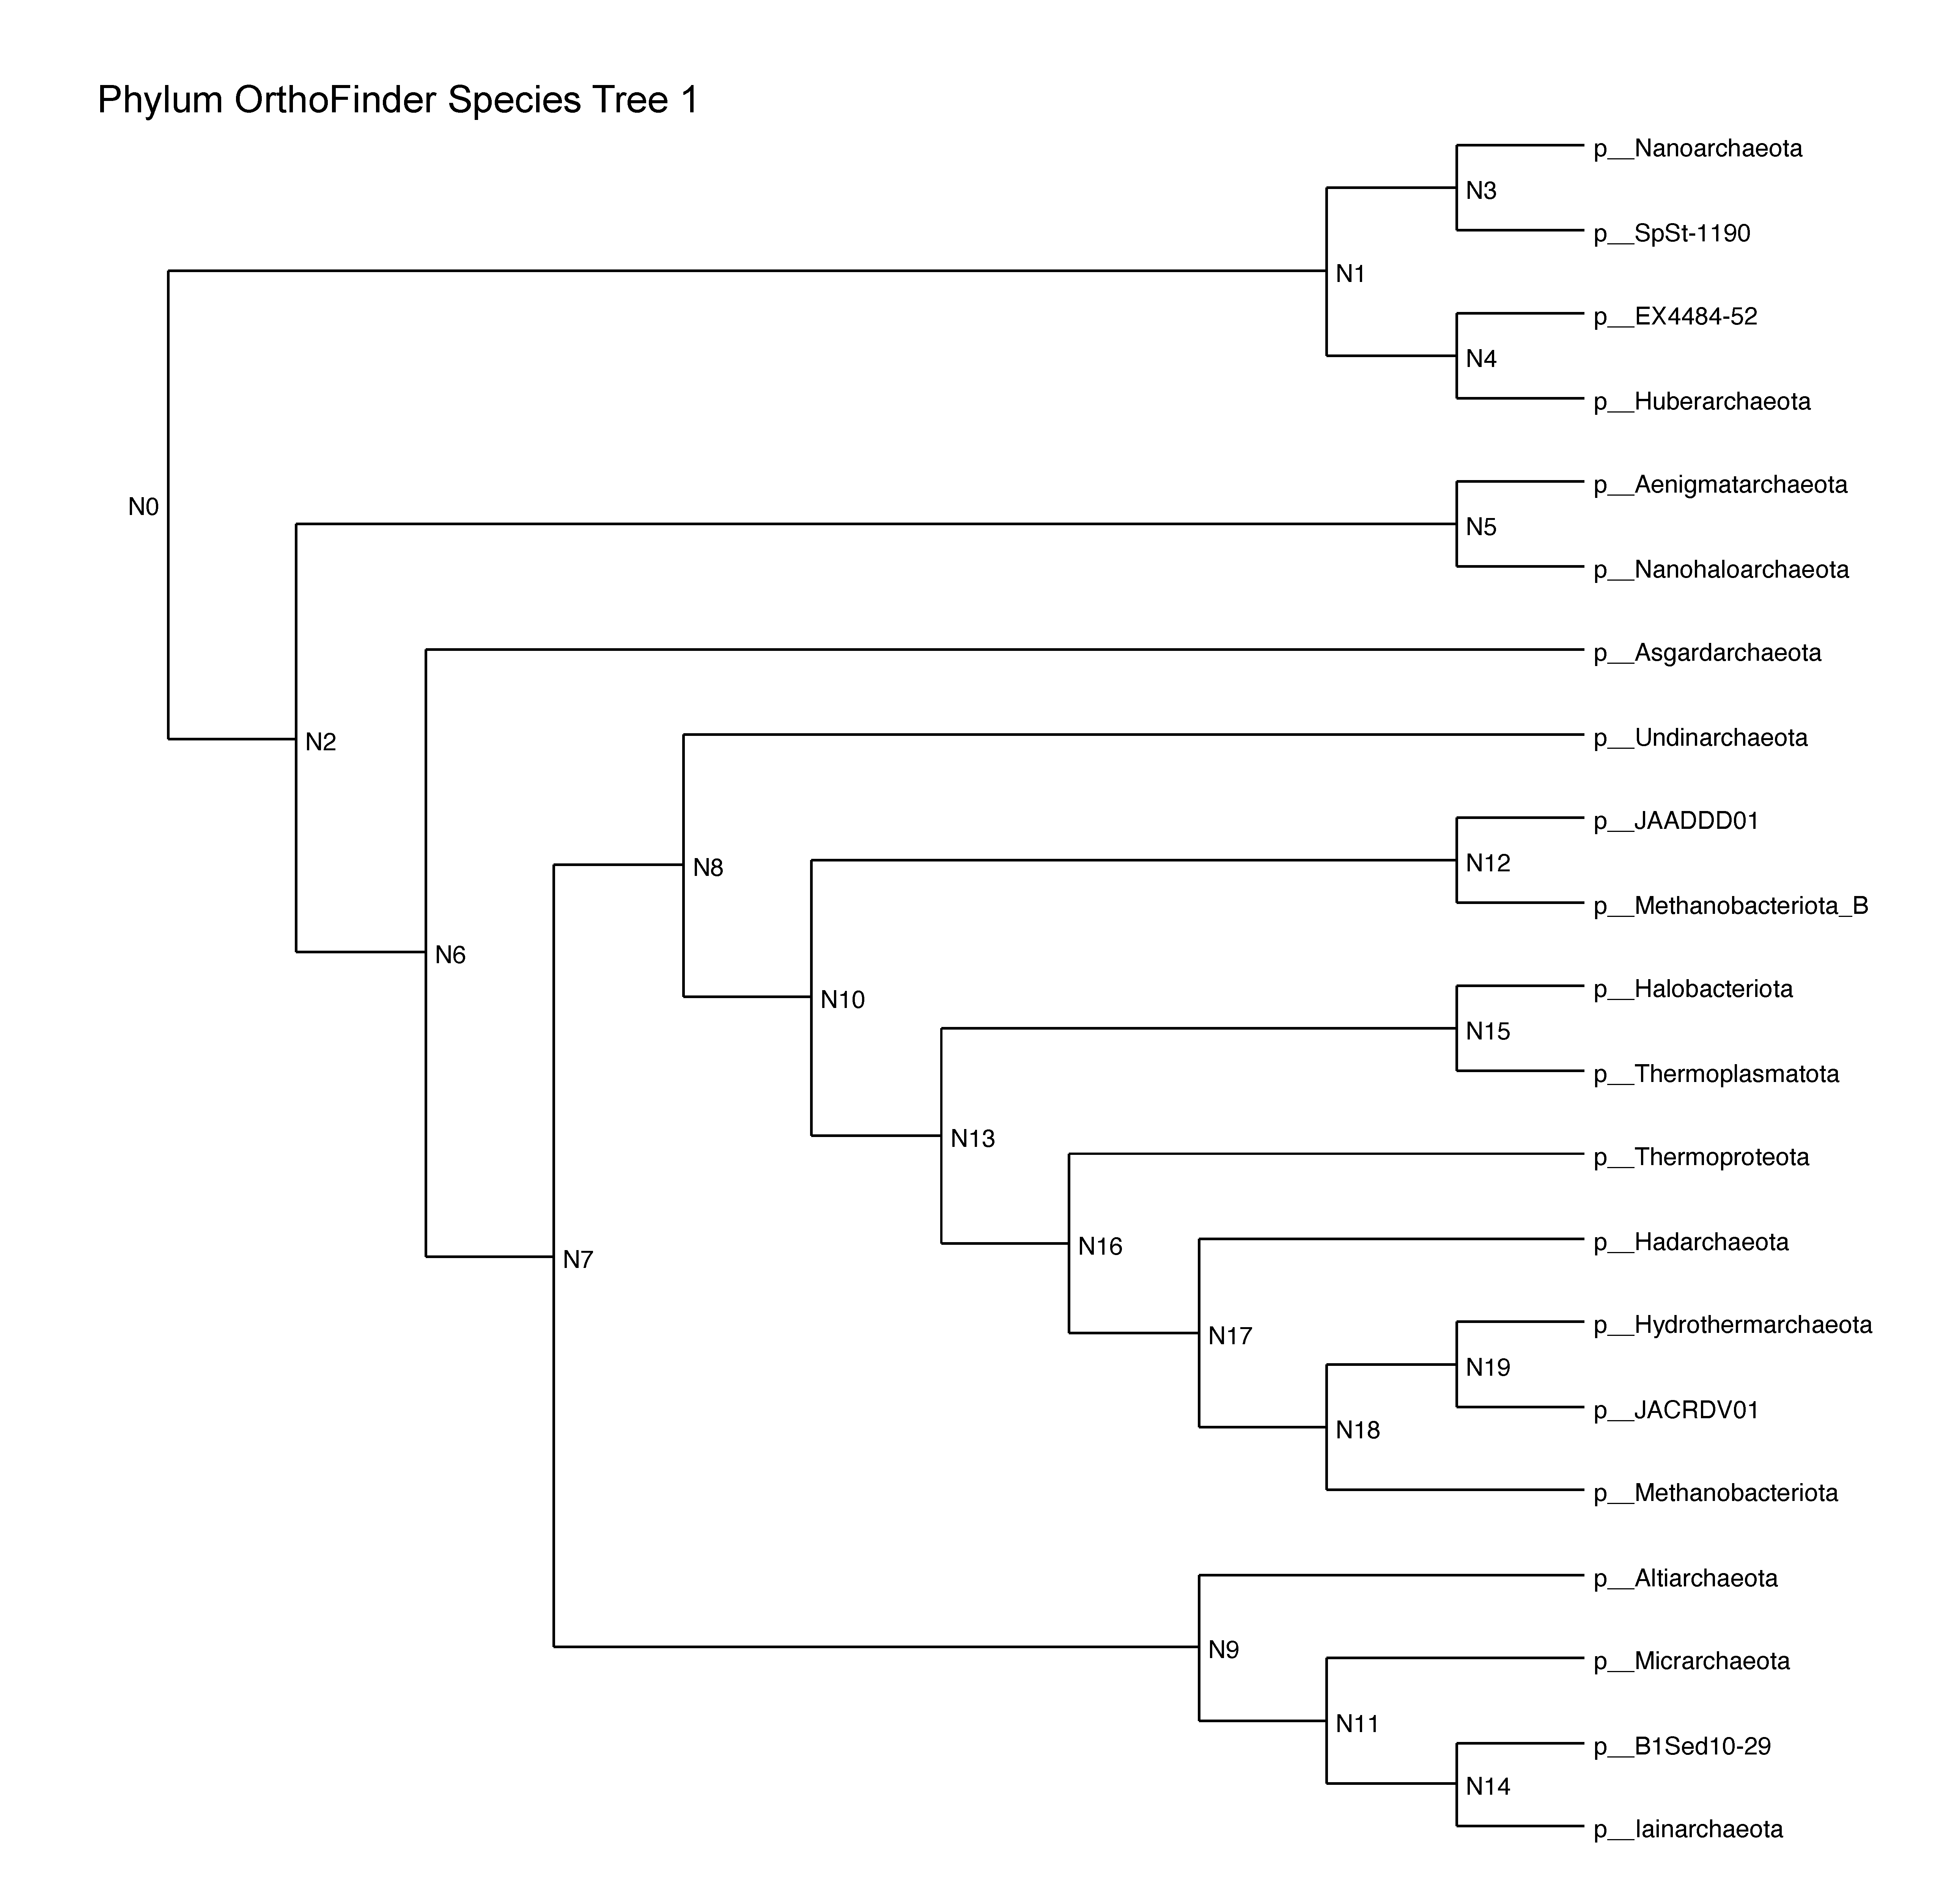
\includegraphics[width=0.5\textwidth]{trees/phy1arc}
    \caption{OrthoFinder-inferred species tree; first analysis.}
    \label{phylum_trees1}
\end{figure}

\begin{figure}[h!tbp]
    \centering
    \renewcommand{\thefigure}{A\arabic{figure}}
    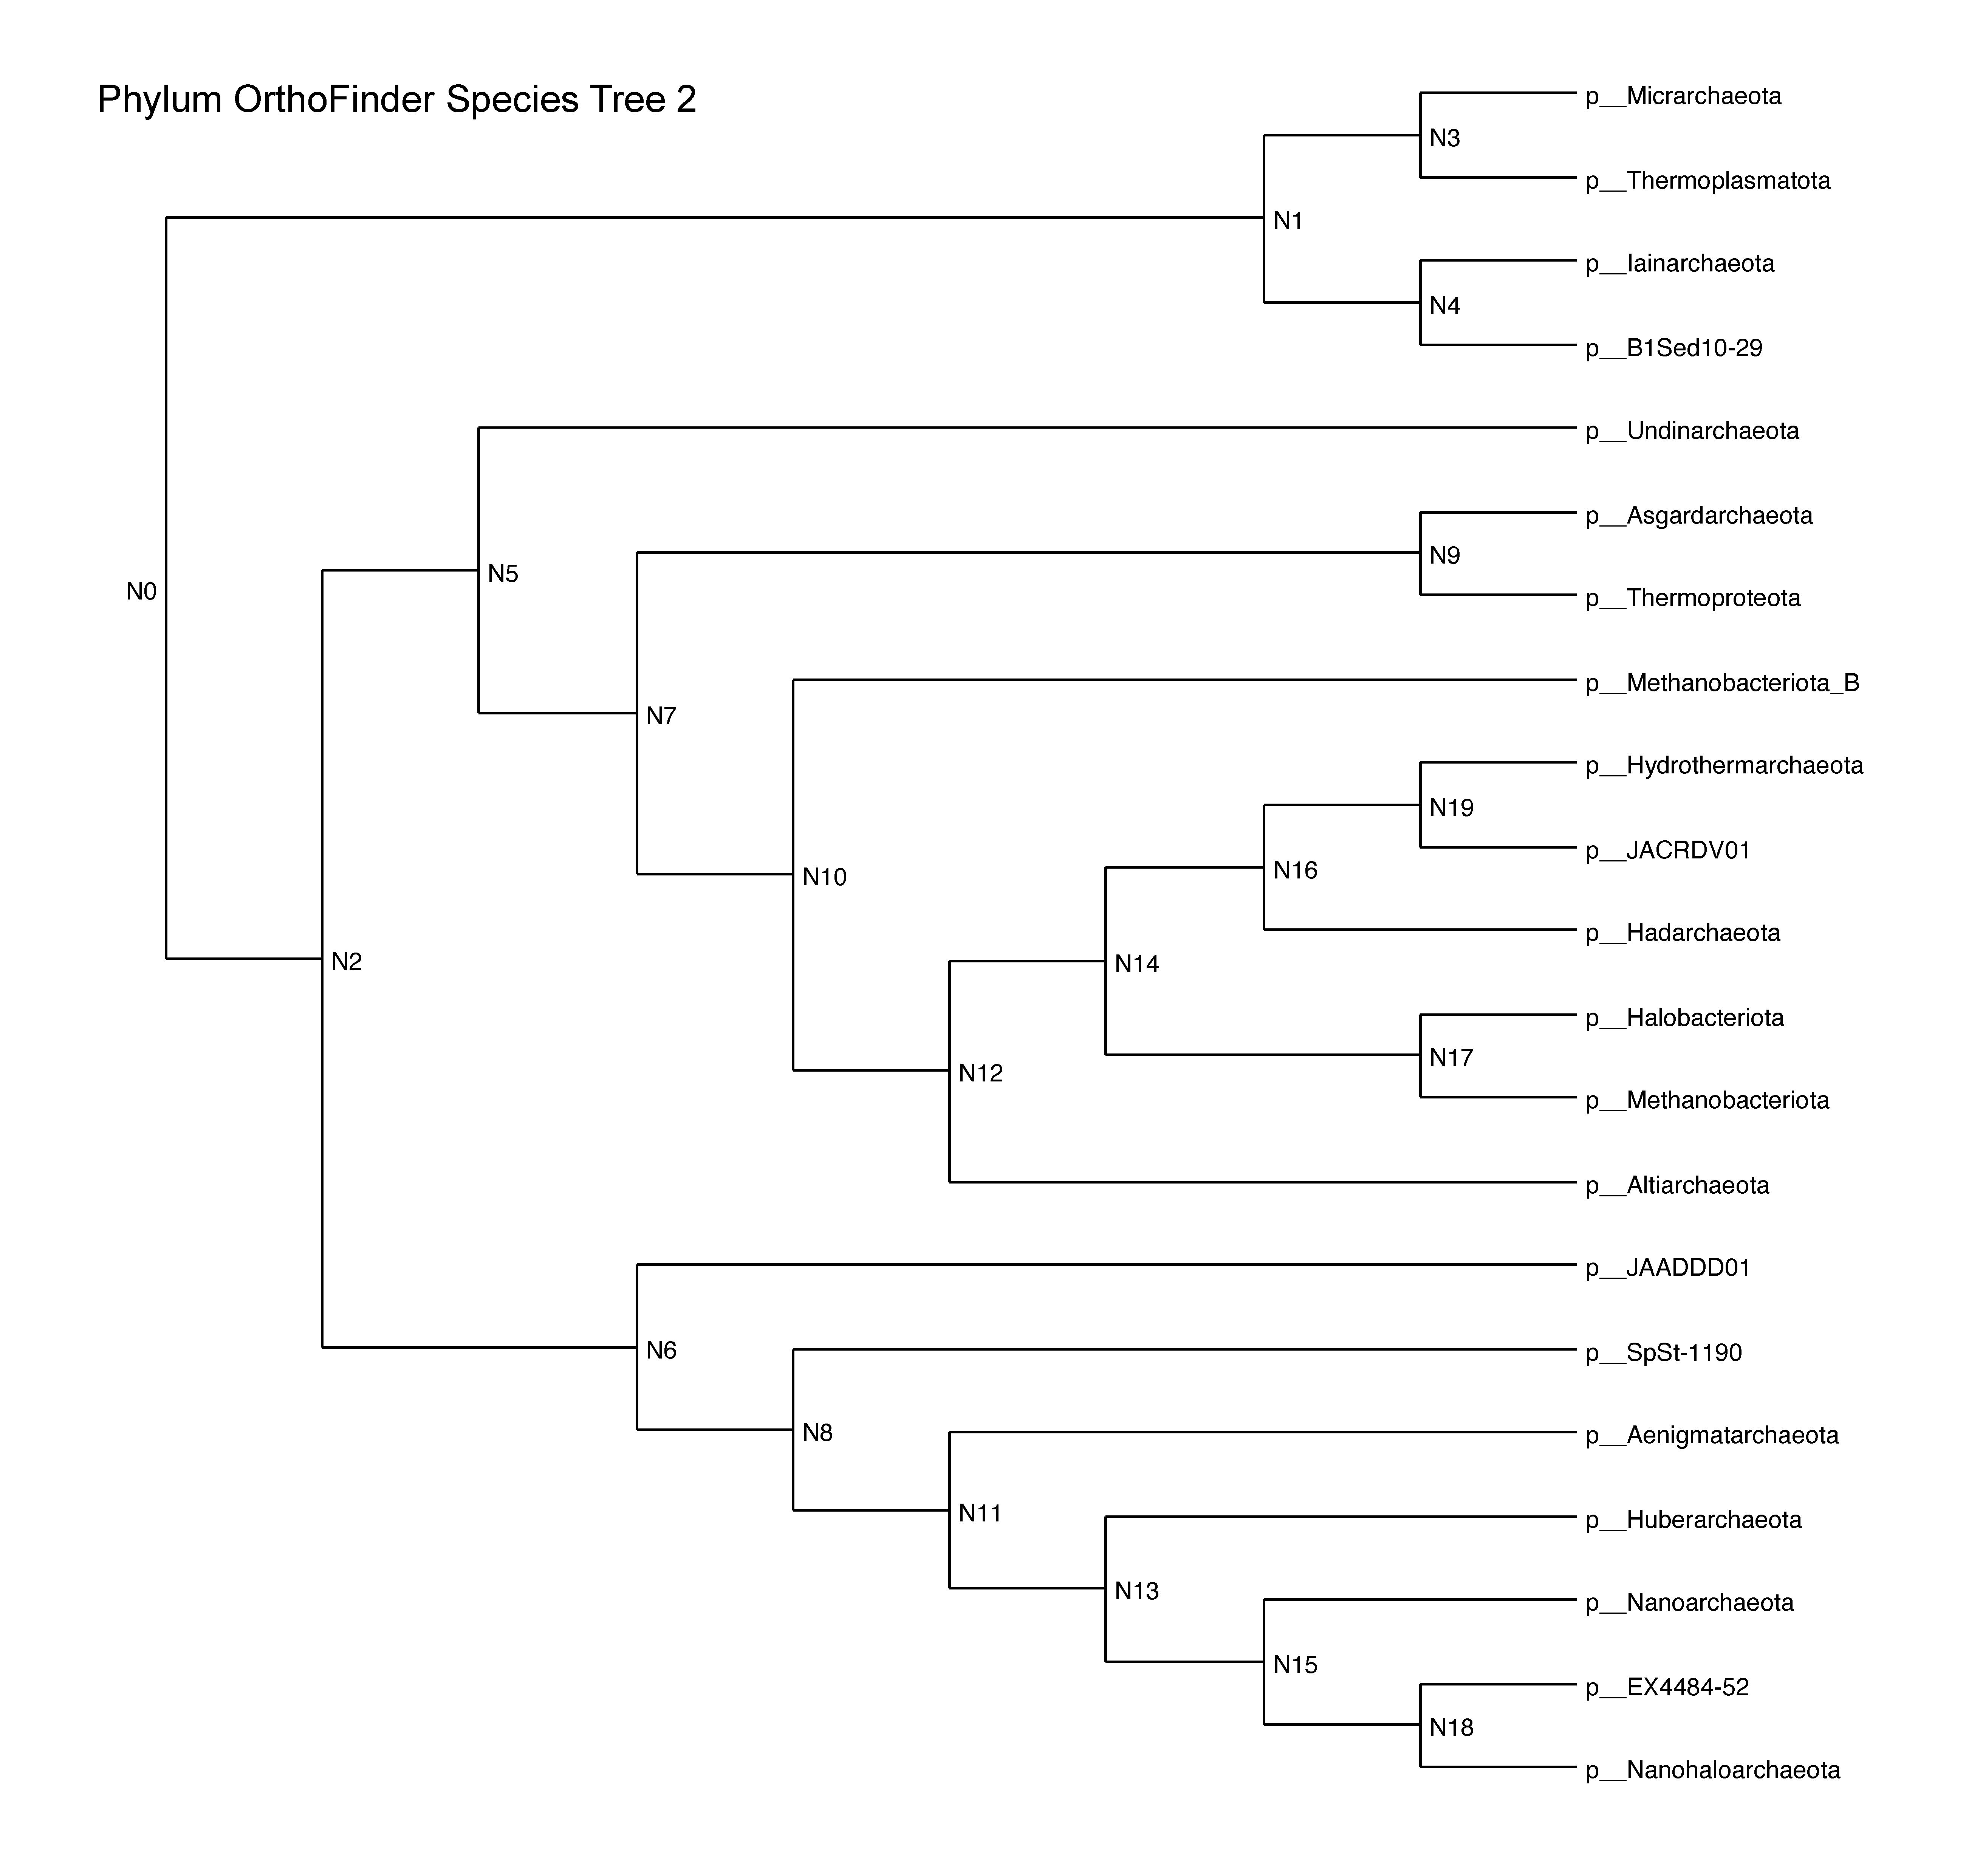
\includegraphics[width=0.5\textwidth]{trees/phy2arc}
    \caption{OrthoFinder-inferred species tree; second analysis.}
    \label{phylum_trees2}
\end{figure}

\begin{figure}[h!tbp]
    \centering
    \renewcommand{\thefigure}{A\arabic{figure}}
    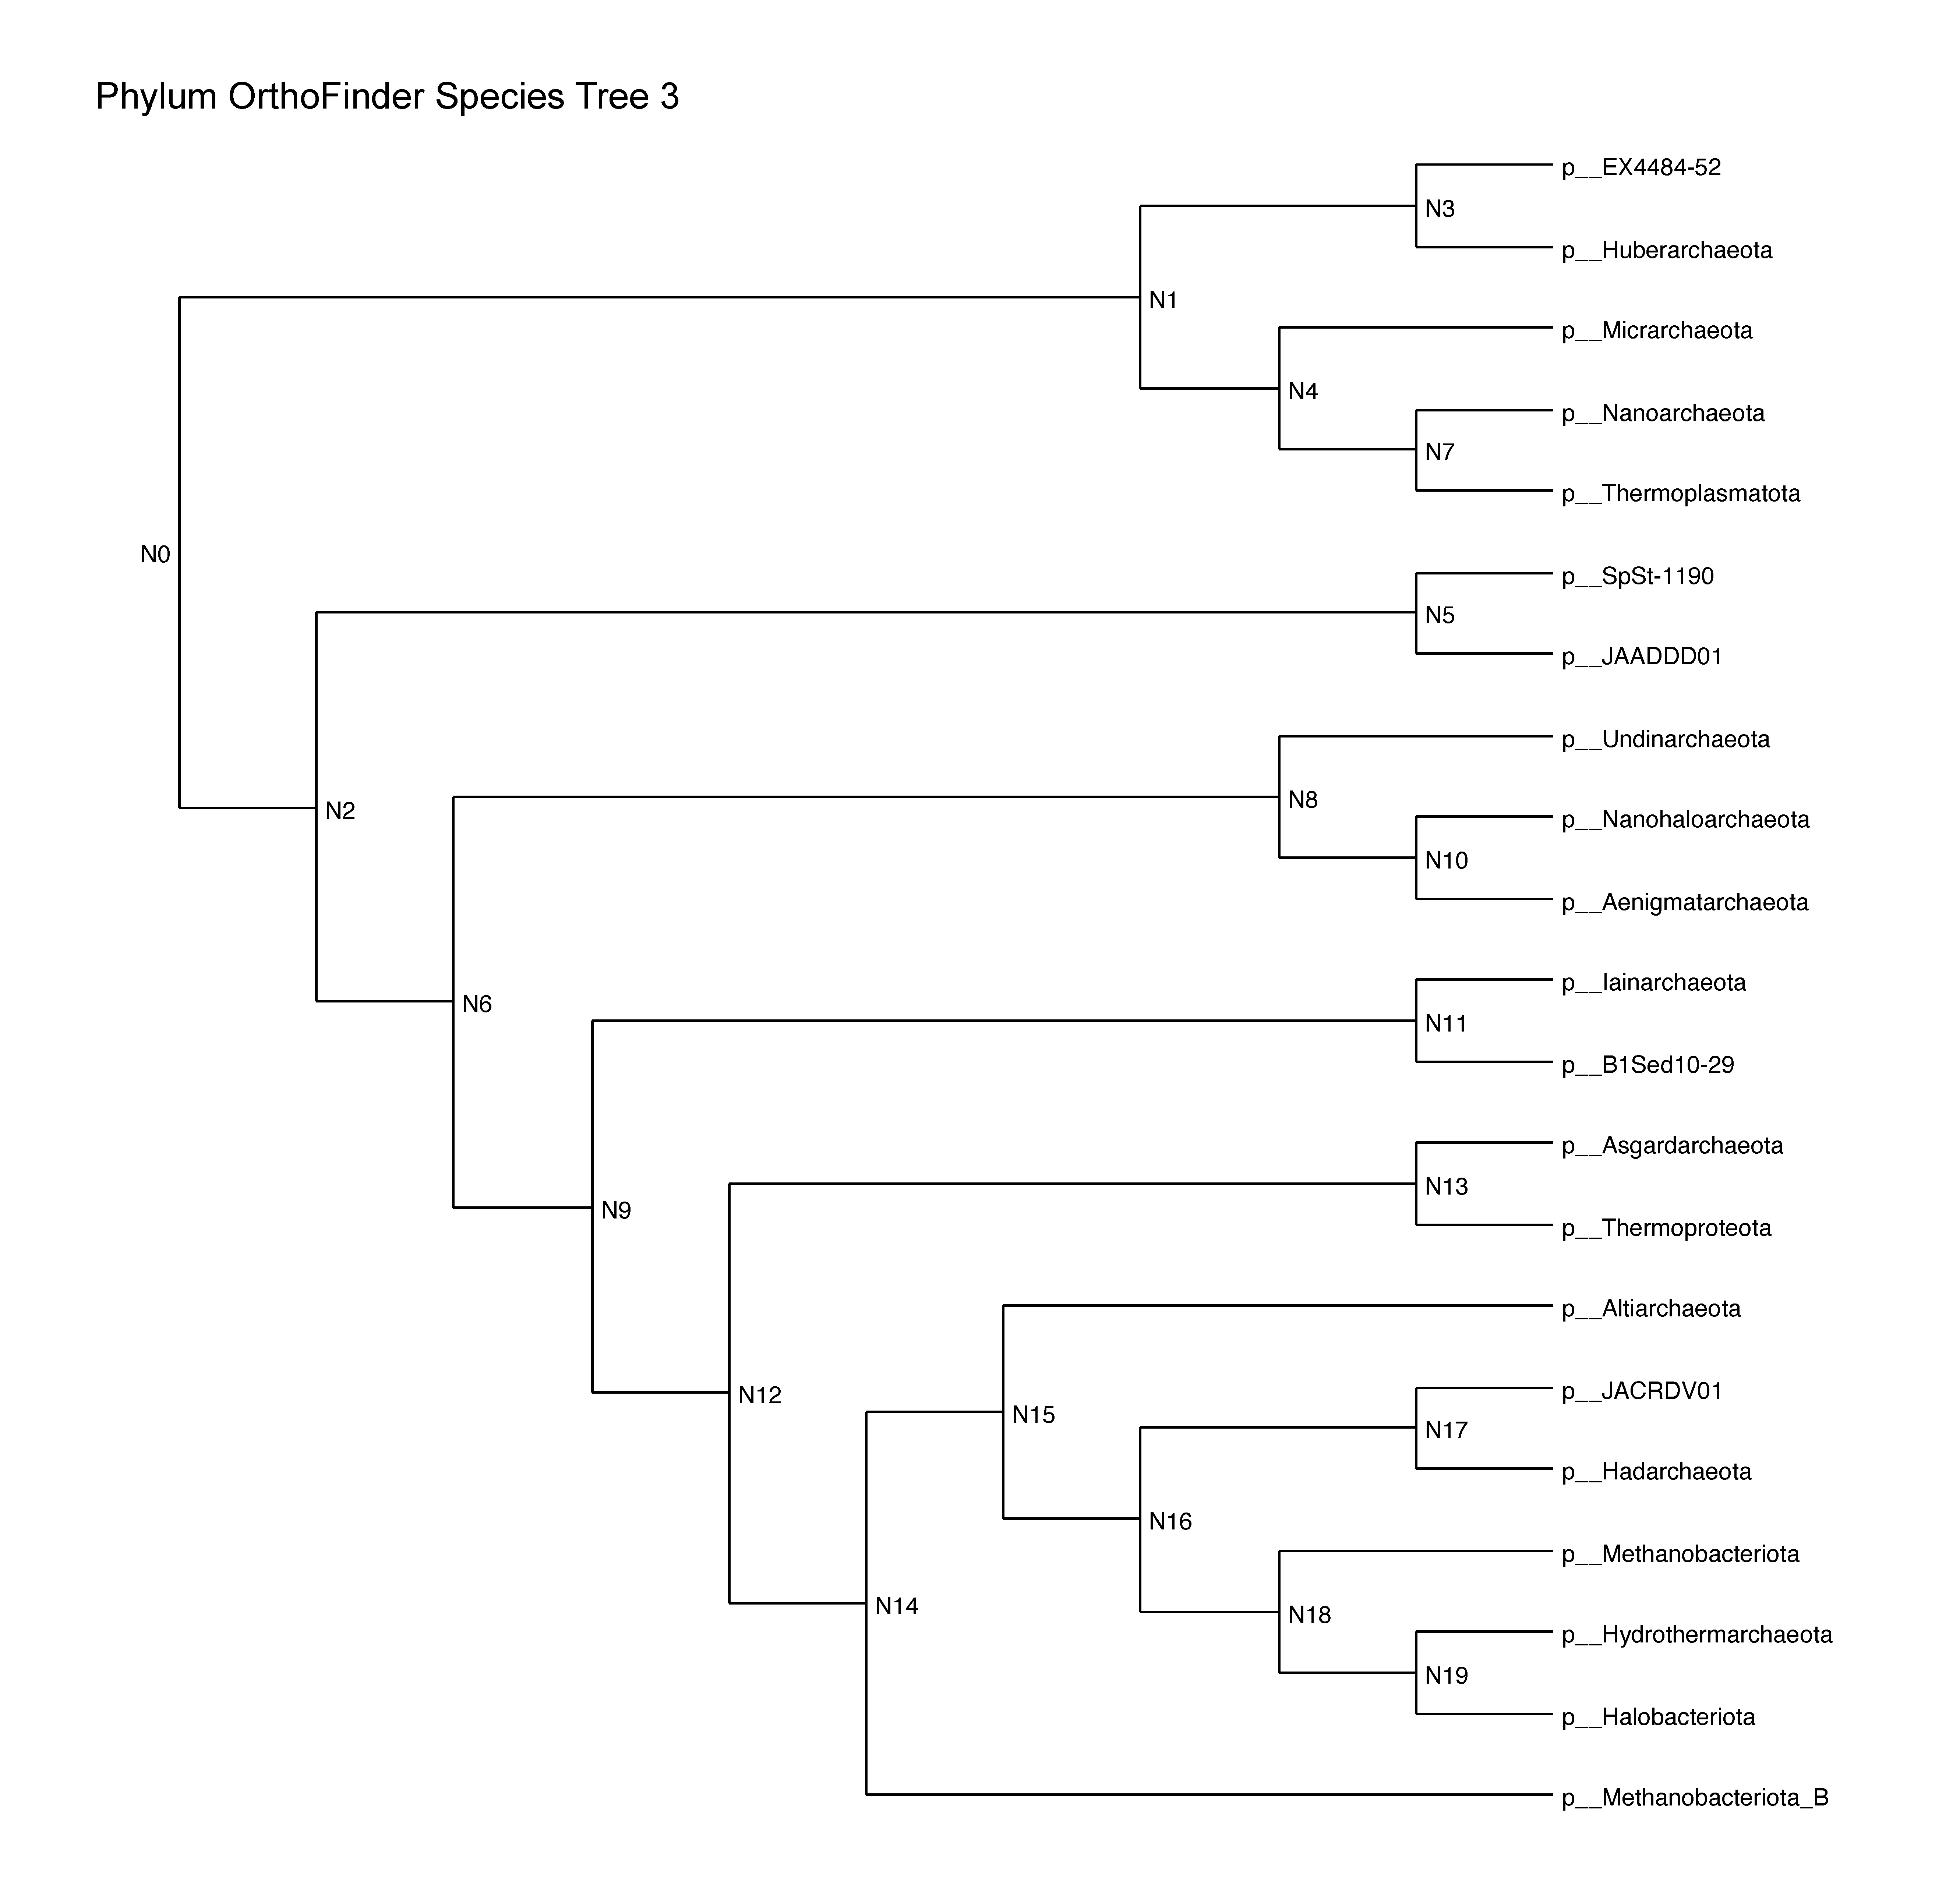
\includegraphics[width=0.6\textwidth]{trees/phy3arc}
    \caption{OrthoFinder-inferred species tree; third analysis.}
    \label{phylum_trees3}
\end{figure}

\begin{figure}[h!tbp]
    \centering
    \renewcommand{\thefigure}{A\arabic{figure}}
    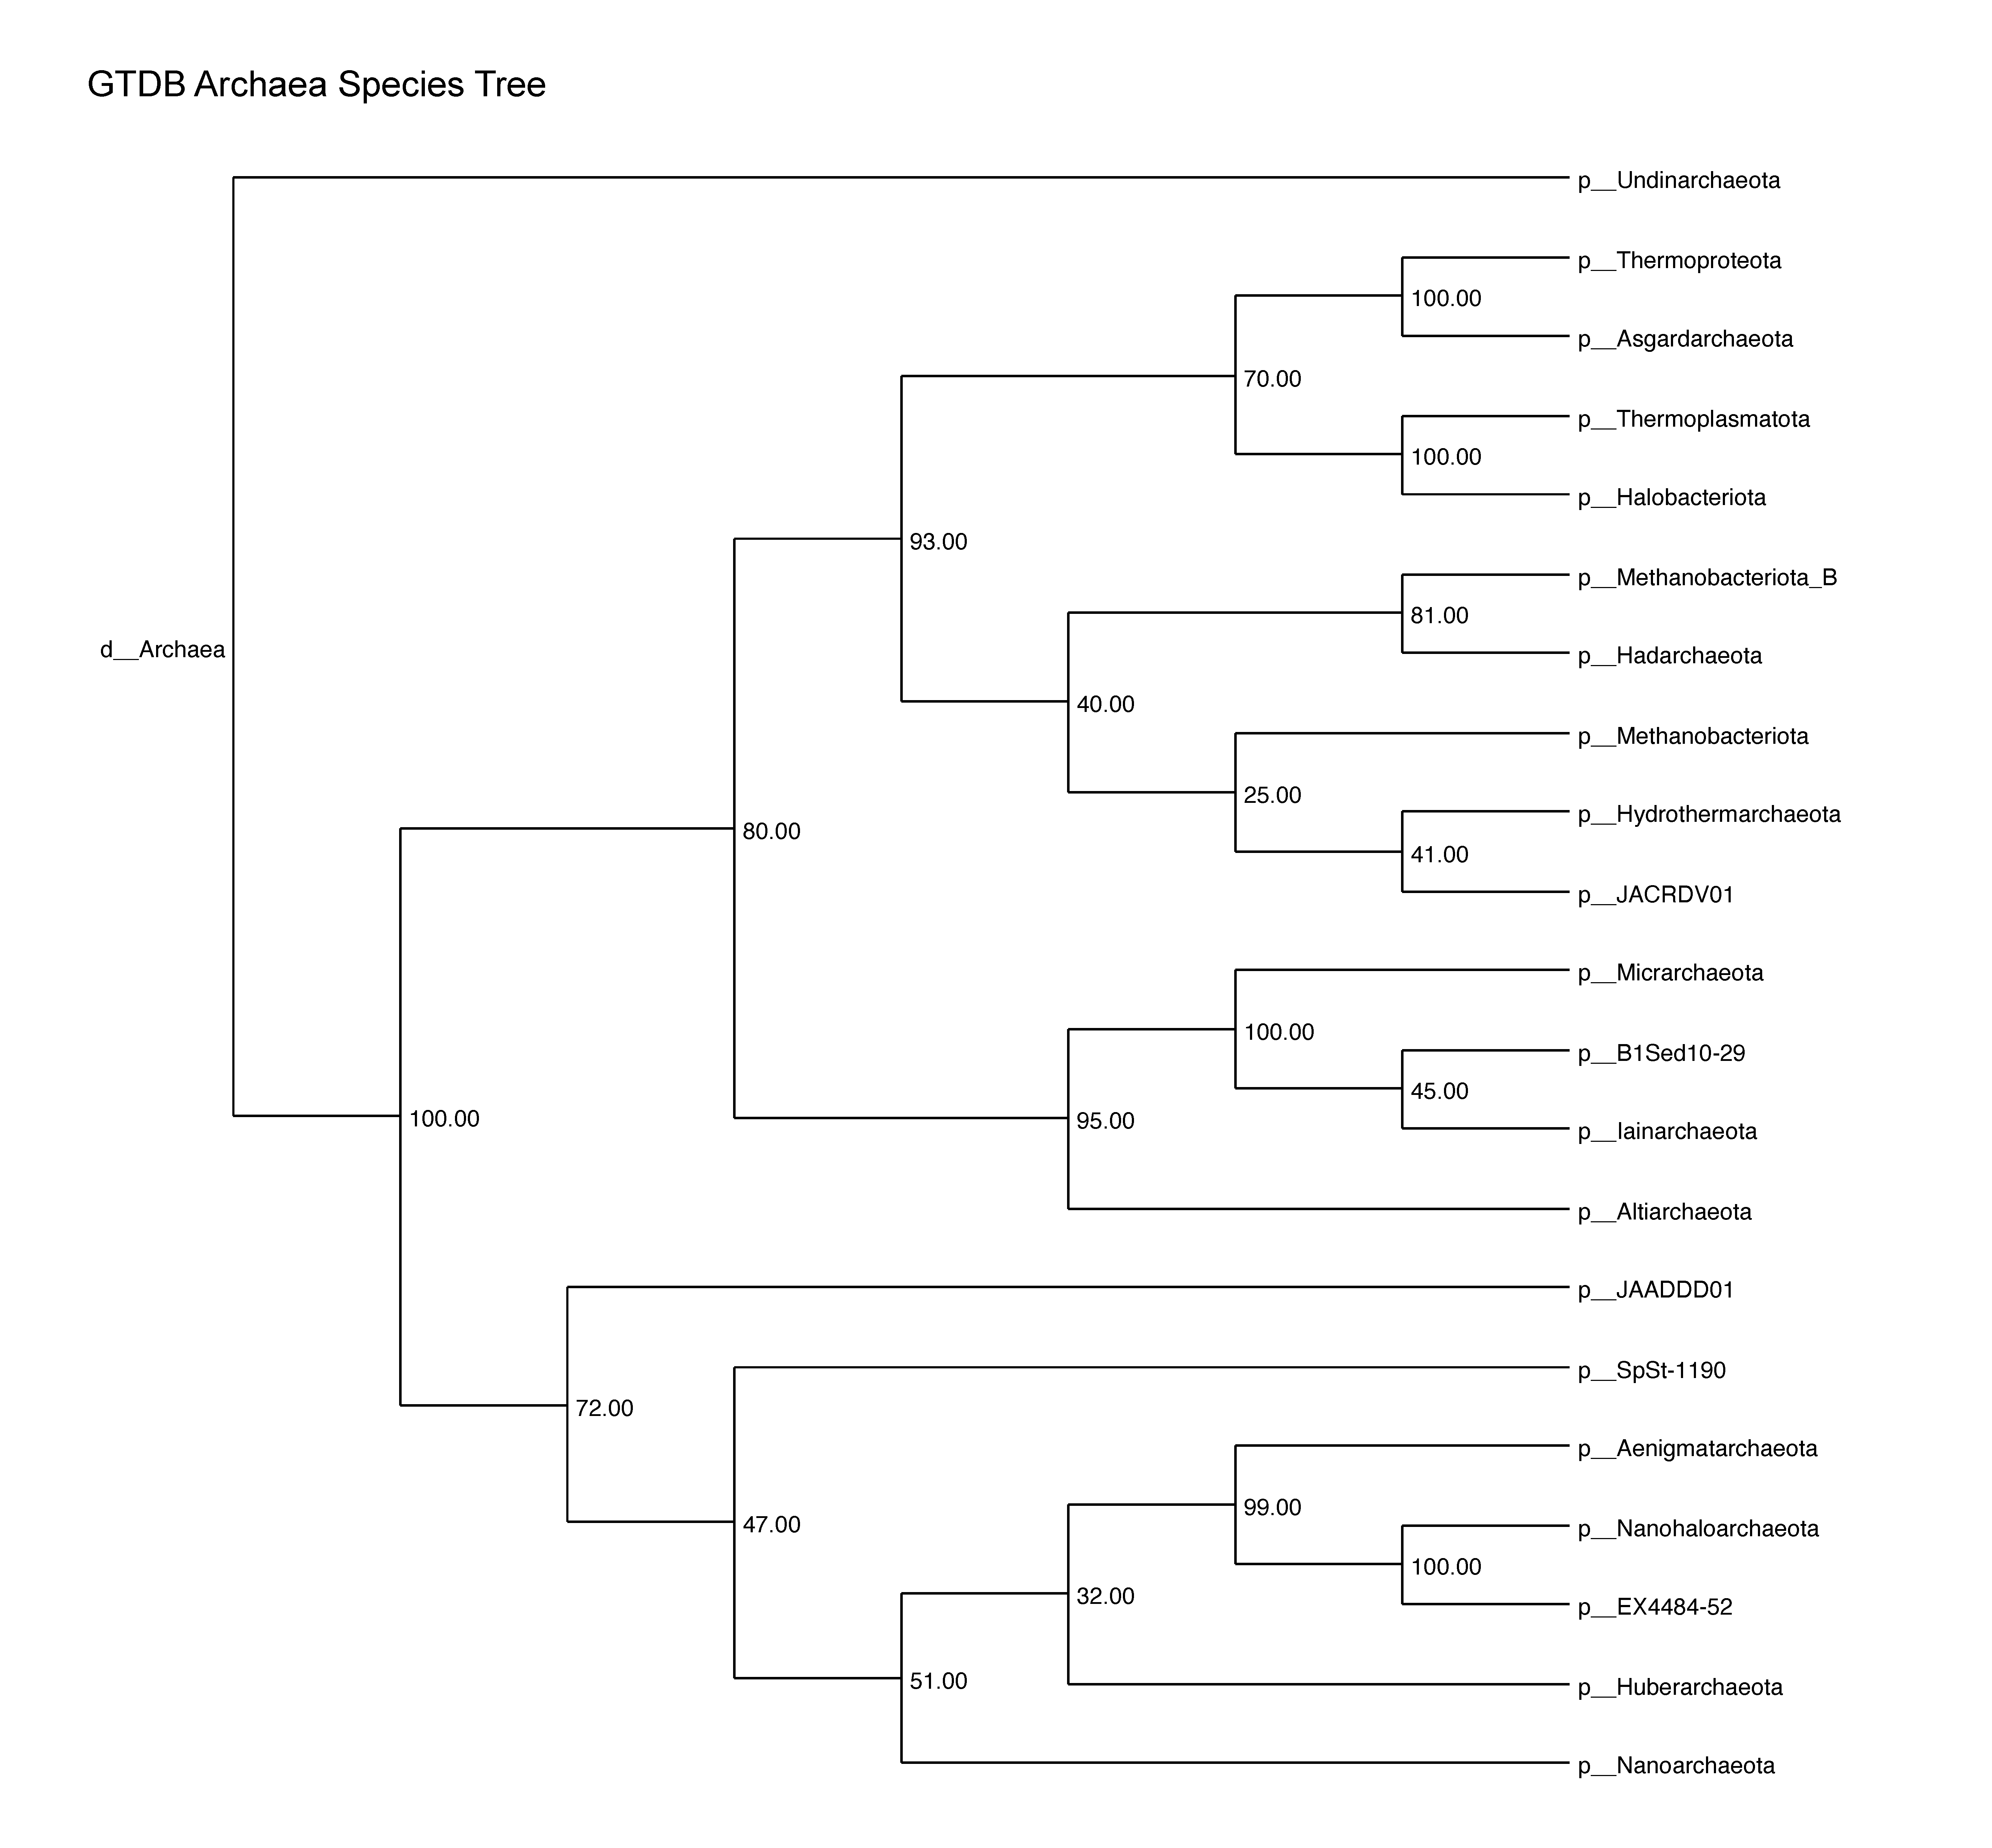
\includegraphics[width=0.6\textwidth]{trees/gtdb_tree}
    \caption{GTDB archaea species tree.}
    \label{gtdb_tree}
\end{figure}

\subsection*{A2. Metabolic Network Reconstruction of LACA for all Archaea Datasets}
\textbf{Metabolic Potential of LACA.}

\begin{figure}[H]
    \centering
    \includegraphics[width=0.95\textwidth]{metabolism/phy_arc_n0.pdf}
    \caption{Phylum level archaea LACA}
    \label{phy4arc_metnet}
\end{figure}   

\begin{figure}[H]
    \centering
    \includegraphics[width=0.95\textwidth]{metabolism/cla_arc_n0.pdf}
    \caption{Class level archaea LACA}
    \label{cla4arc_metnet}
\end{figure}   

\begin{figure}[H]
    \centering
    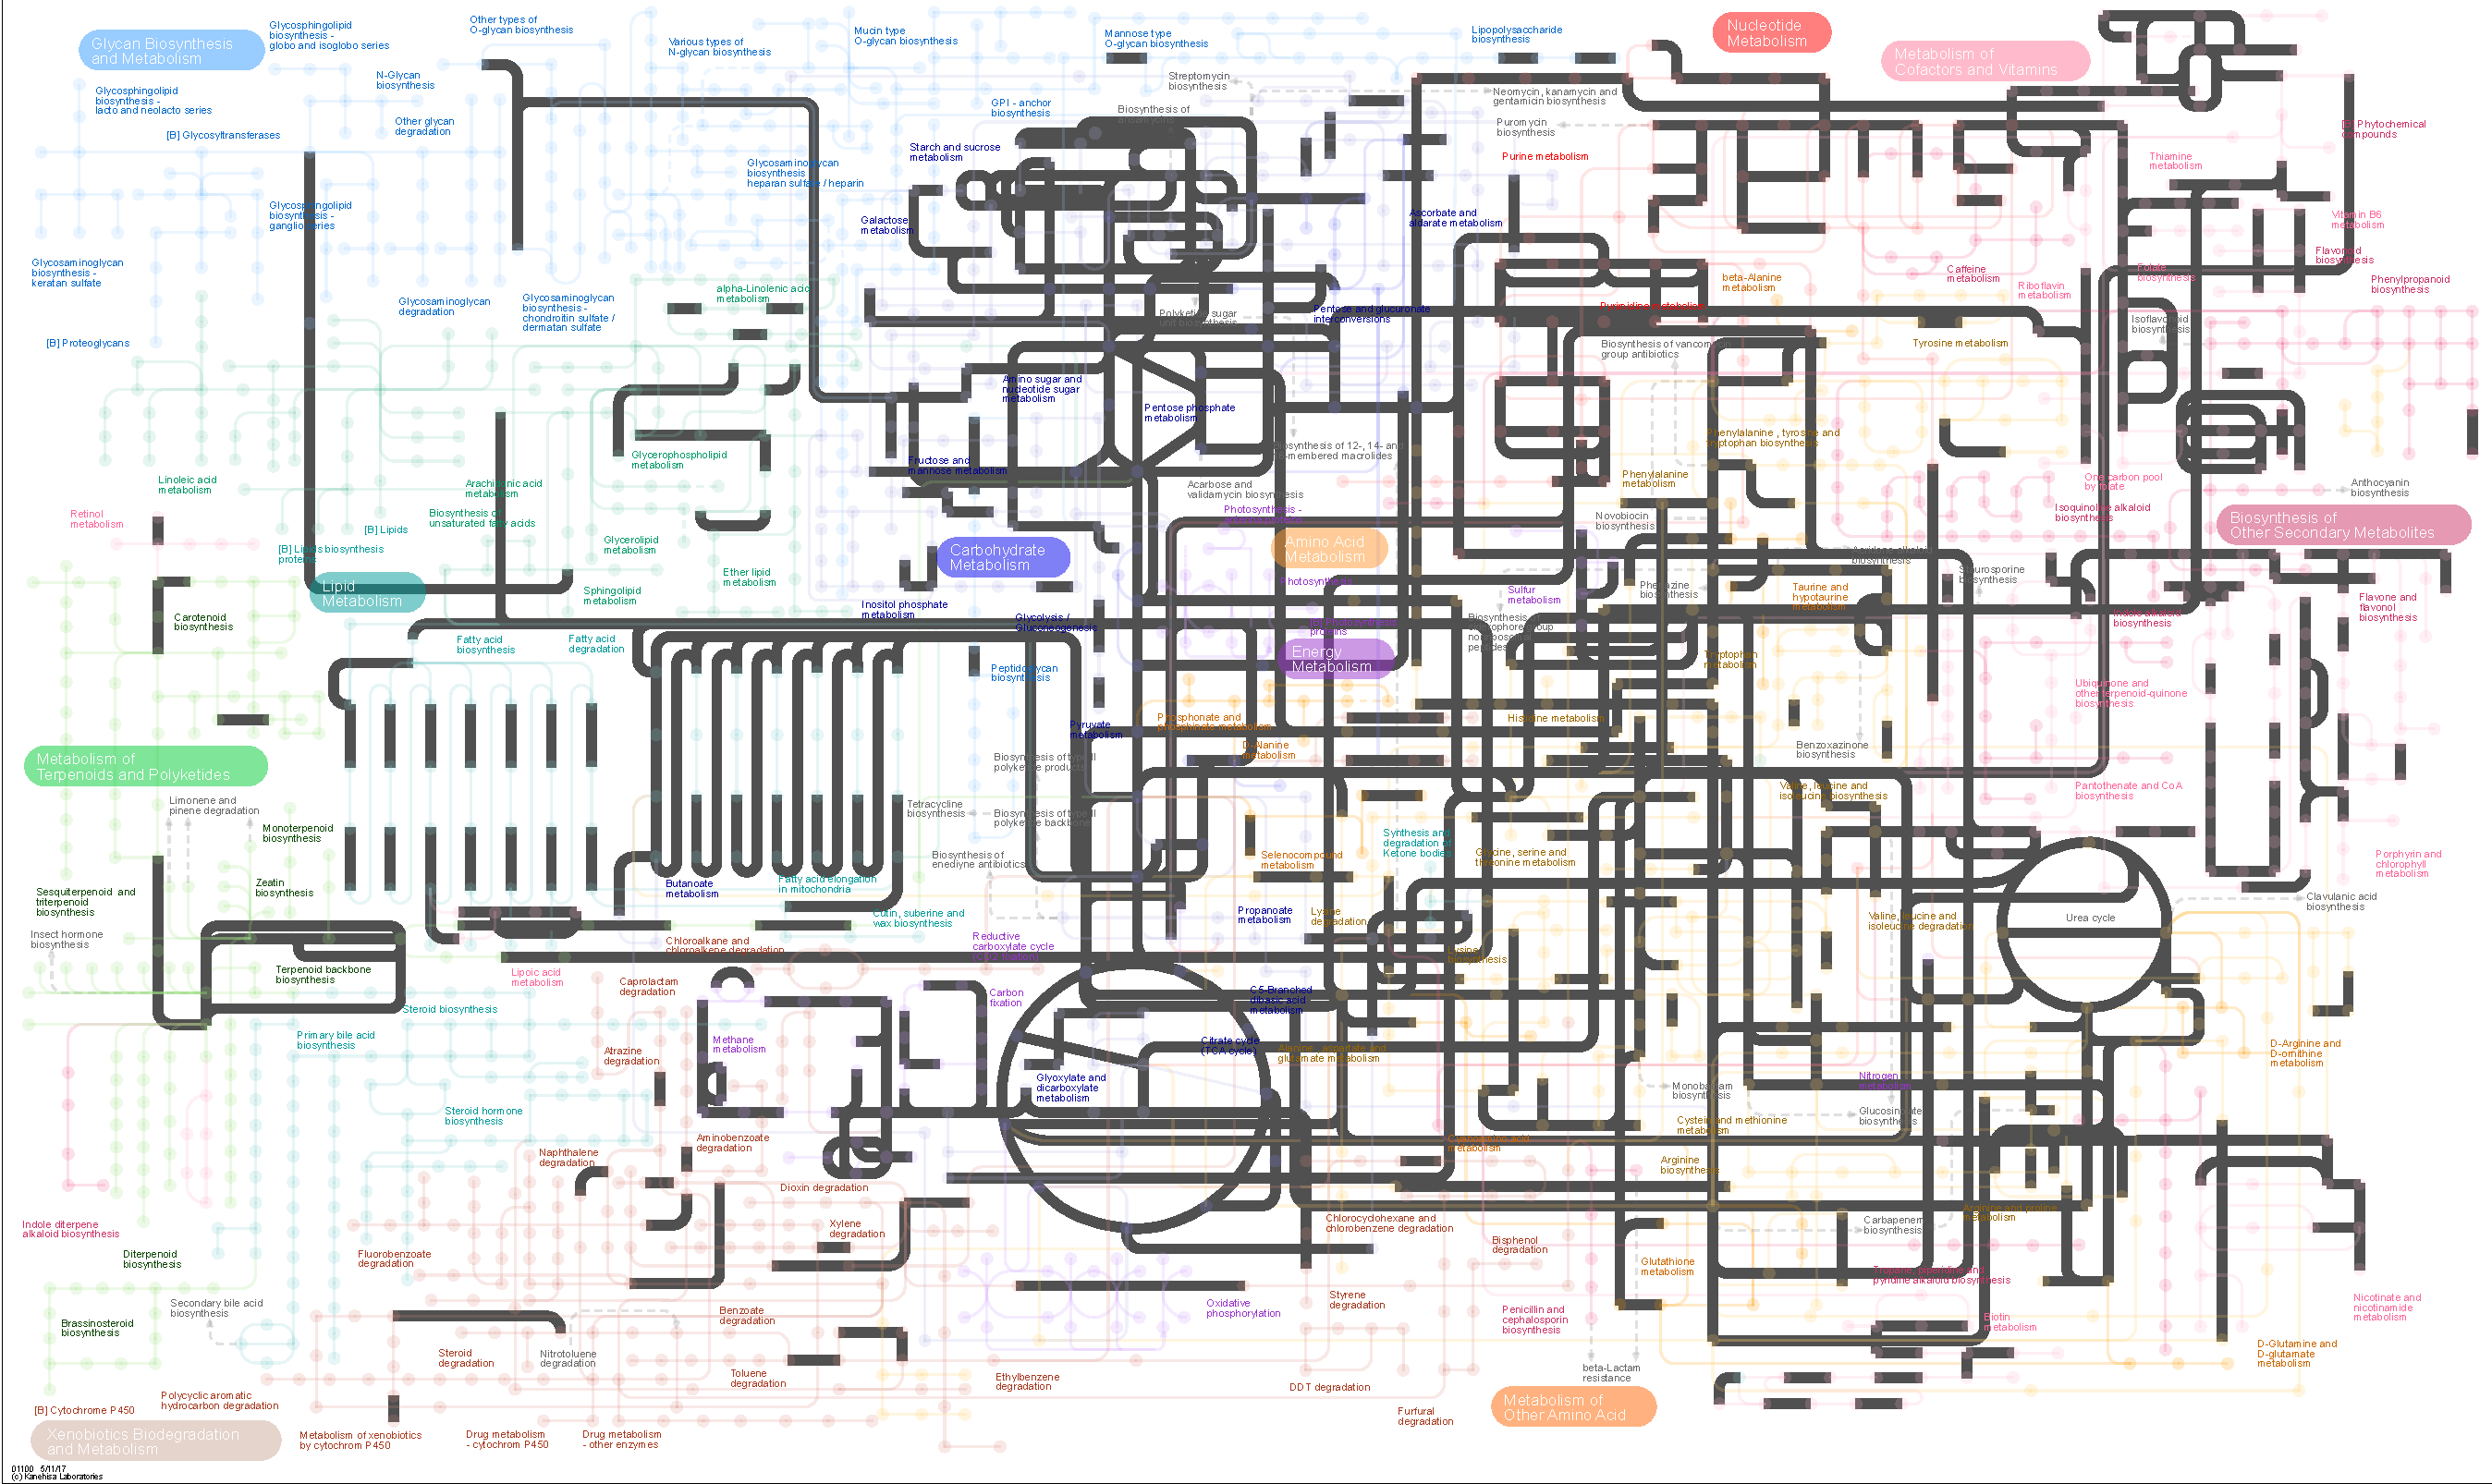
\includegraphics[width=0.95\textwidth]{metabolism/ord_arc_n0.pdf}
    \caption{Order level archaea LACA}
    \label{ord4arc_metnet}
\end{figure}   

\begin{figure}[H]
    \centering
    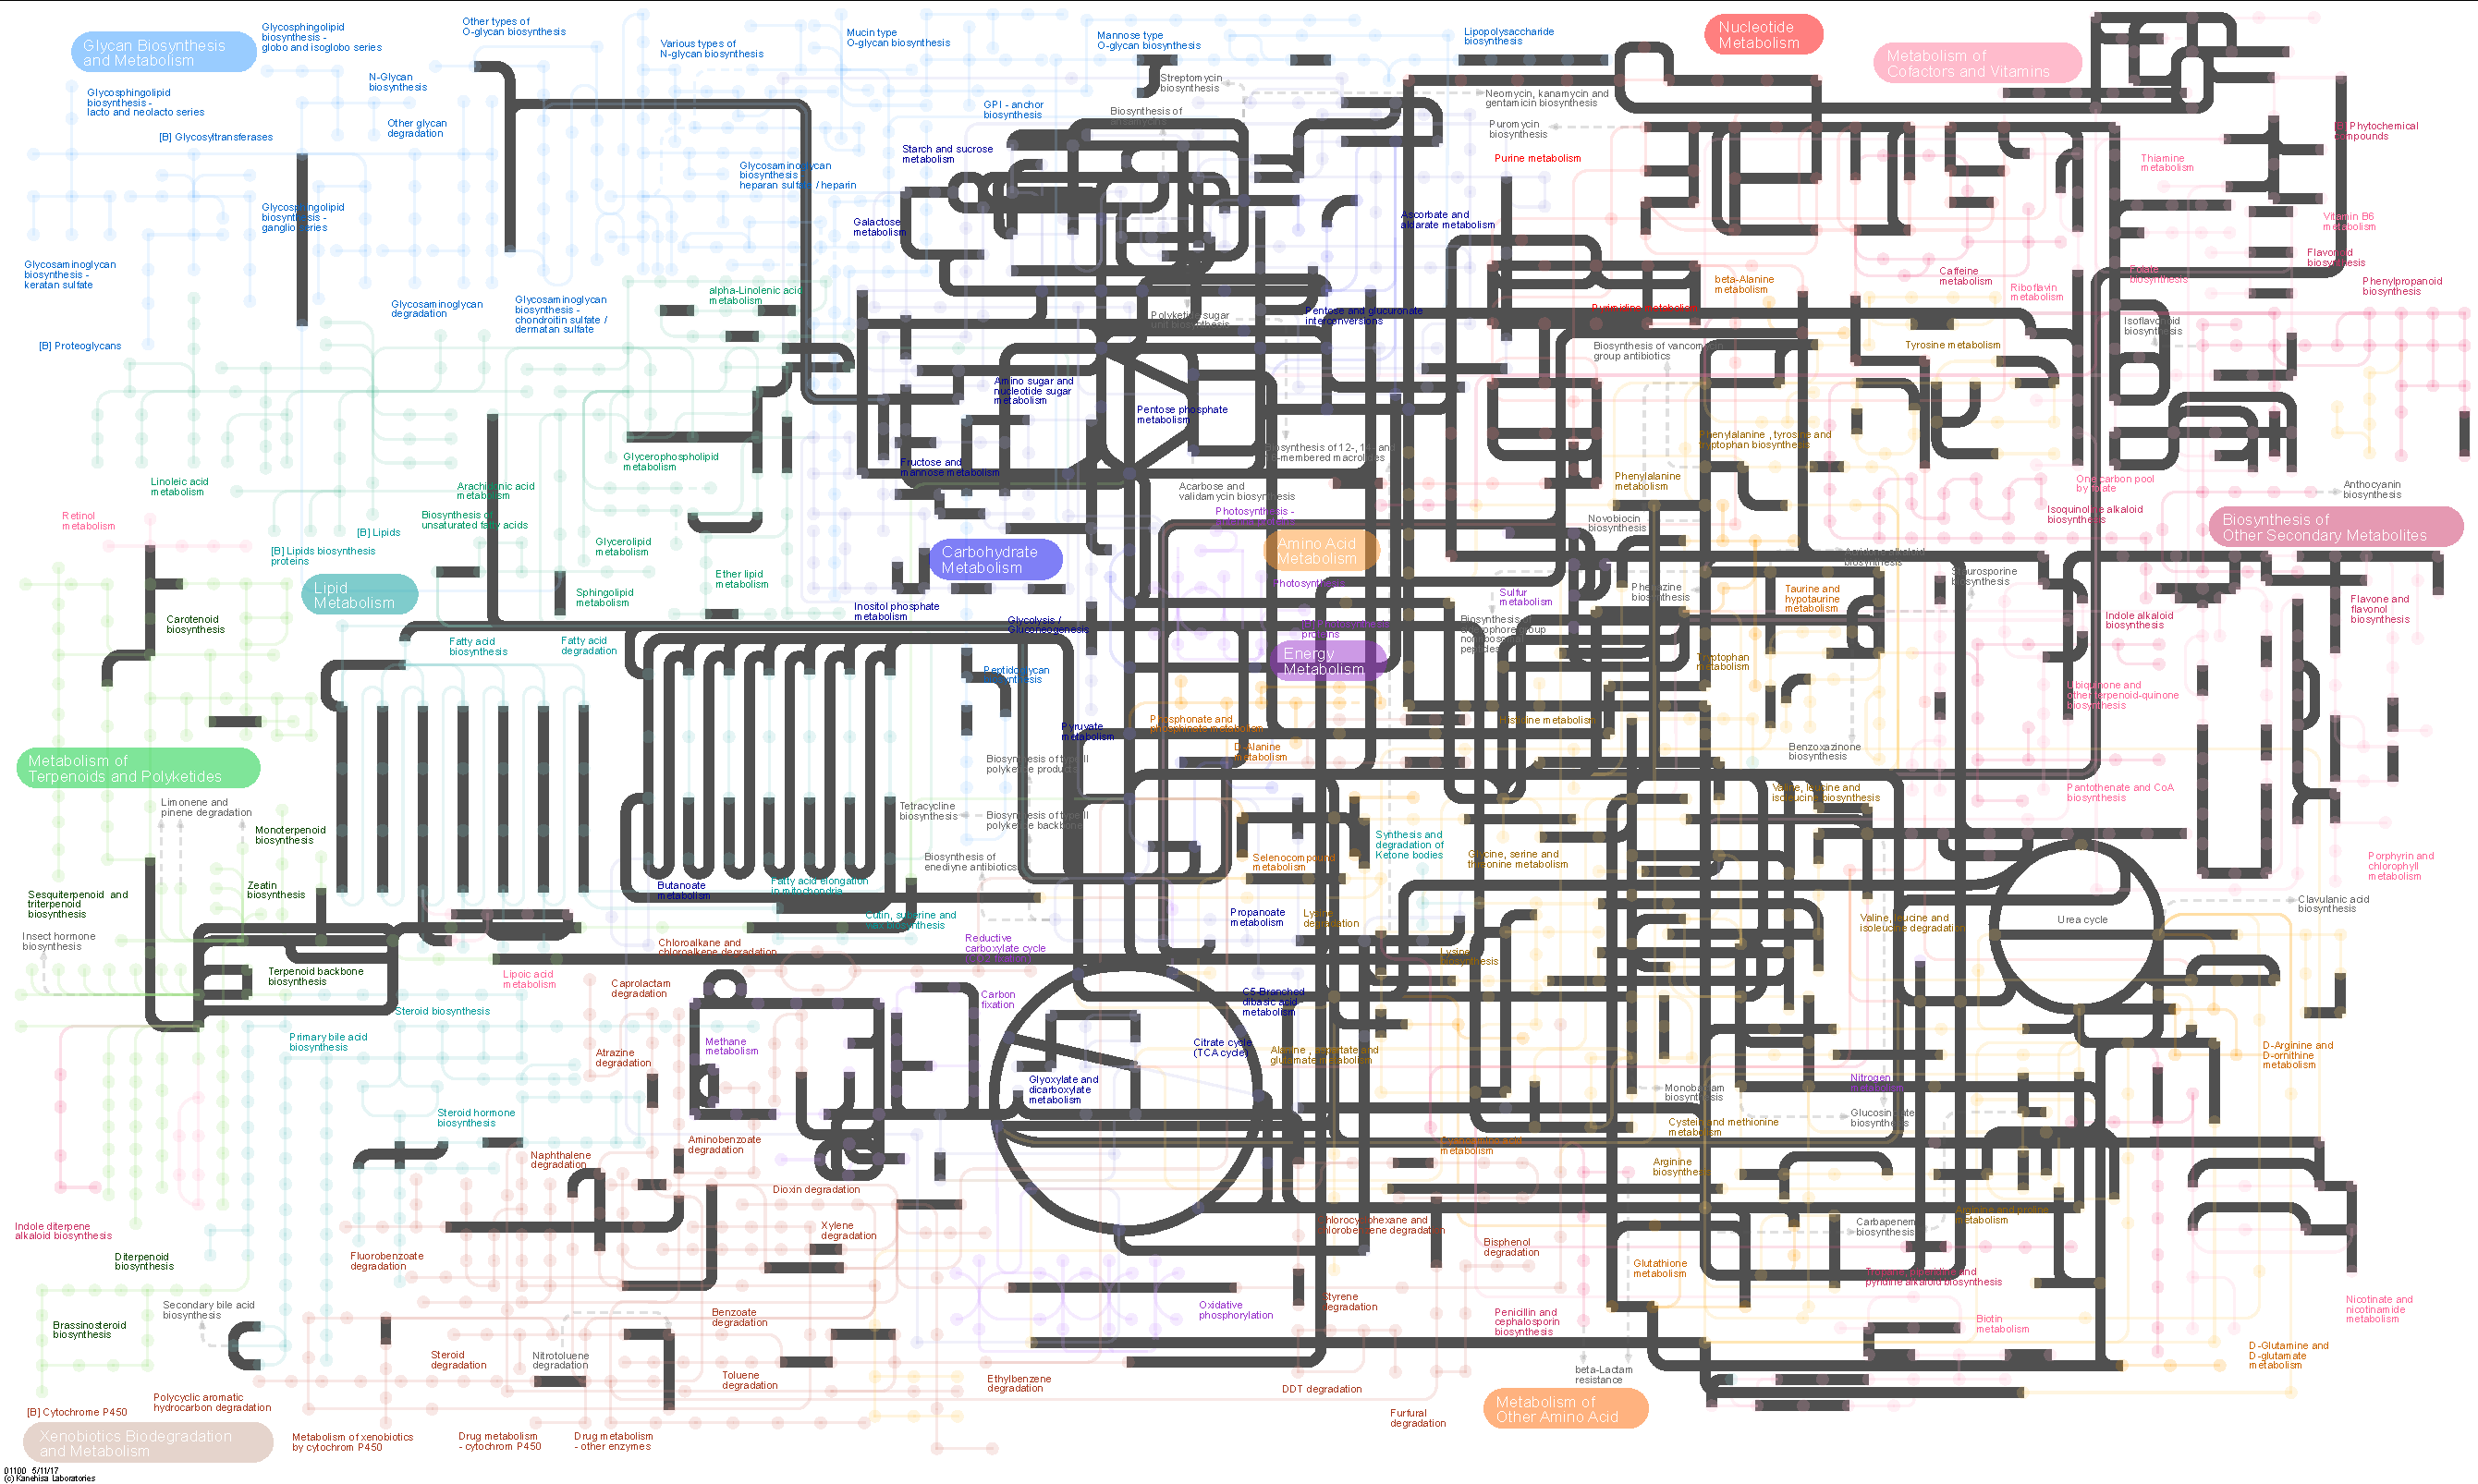
\includegraphics[width=0.95\textwidth]{metabolism/gen_arc_n0.pdf}
    \caption{Genus level archaea LACA}
    \label{gen4arc_metnet}
\end{figure}   

\textbf{EC number evolution in LACA.}
\begin{figure}[H]
    \centering
    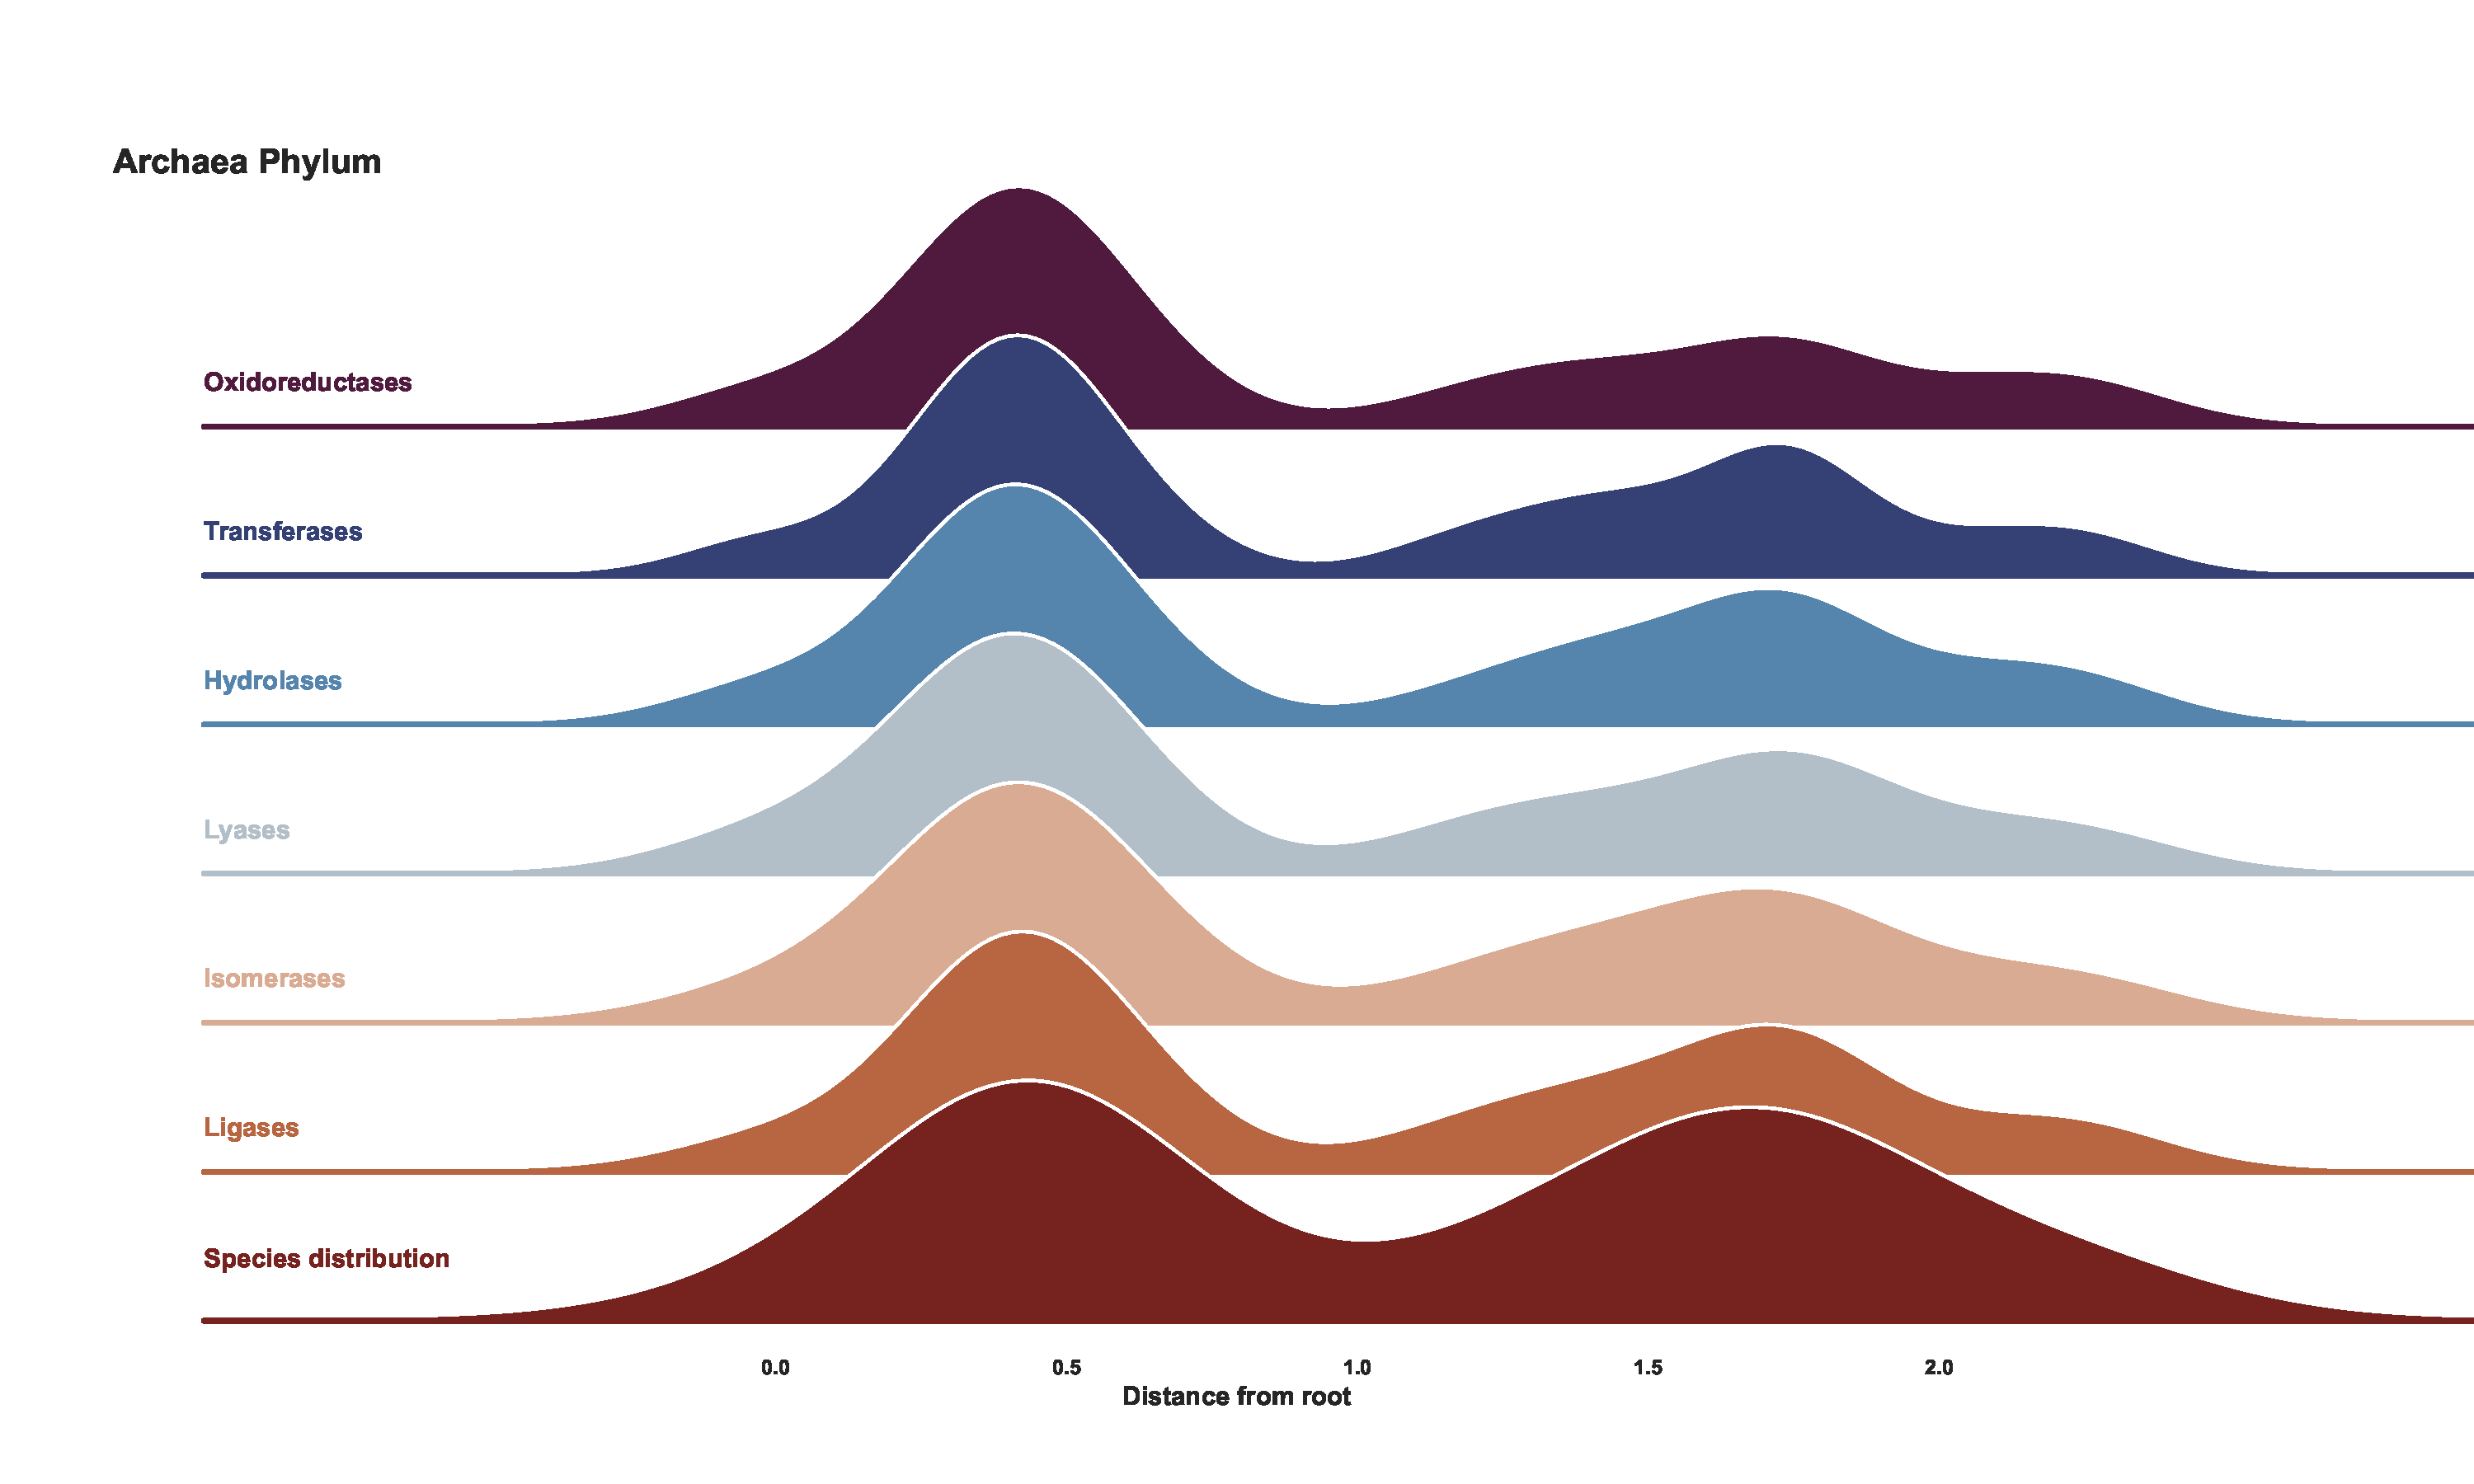
\includegraphics[width=0.95\textwidth]{ridgeplots/phy4arc_ridgeplot.pdf}
    \label{ridgeplot_phy4arc}
\end{figure}

\begin{figure}[H]
    \centering
    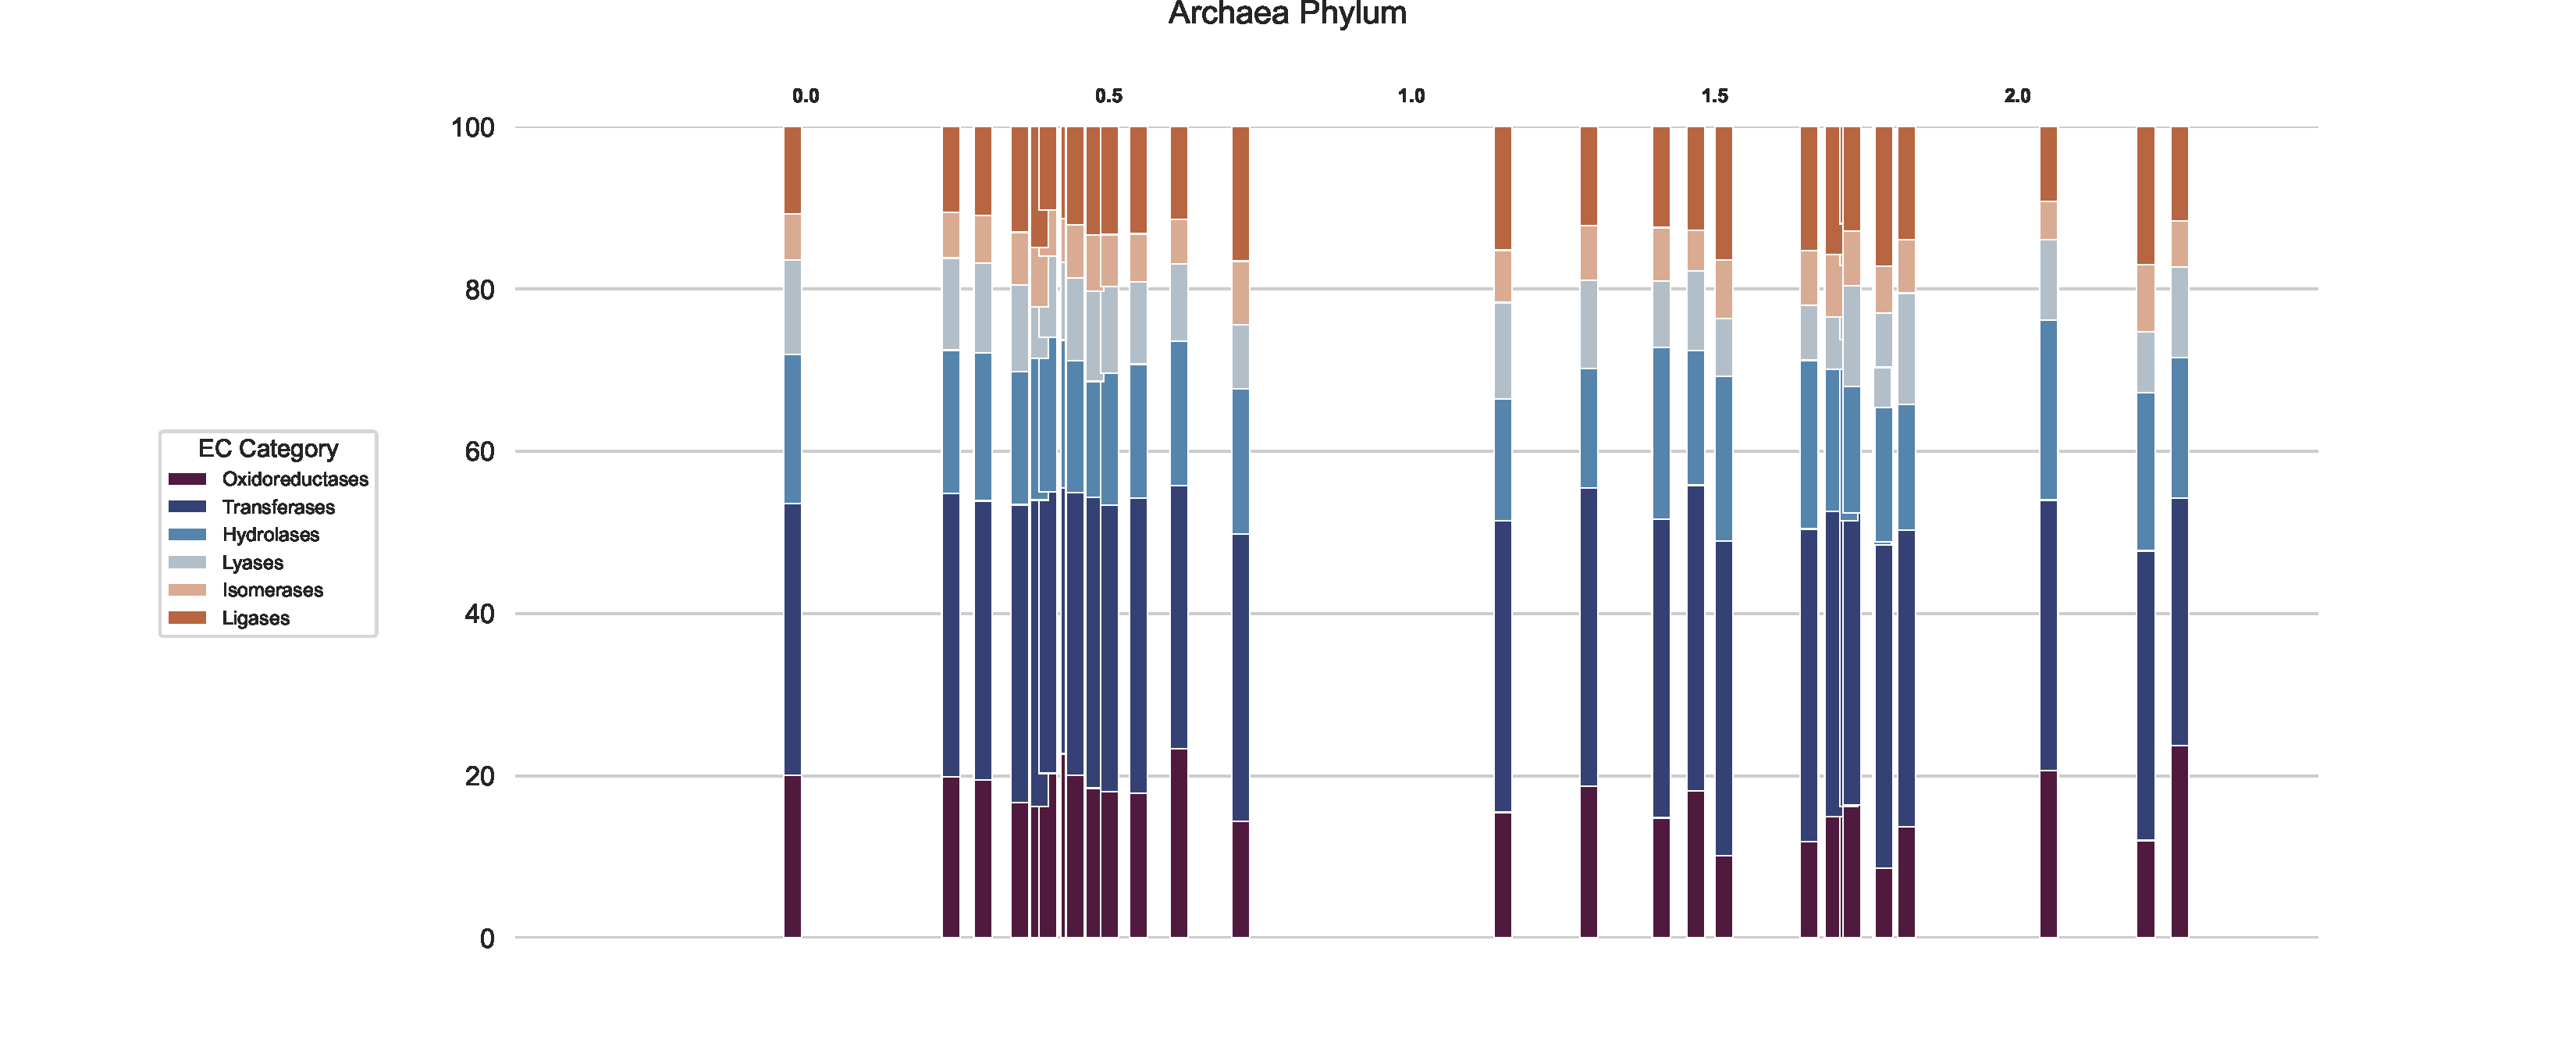
\includegraphics[width=0.95\textwidth]{ridgeplots/phy4arc_barplot.pdf}
    \caption[]{Phylum level archaea}
    \label{barplot_phy4arc}
\end{figure}

\begin{figure}[H]
    \centering
    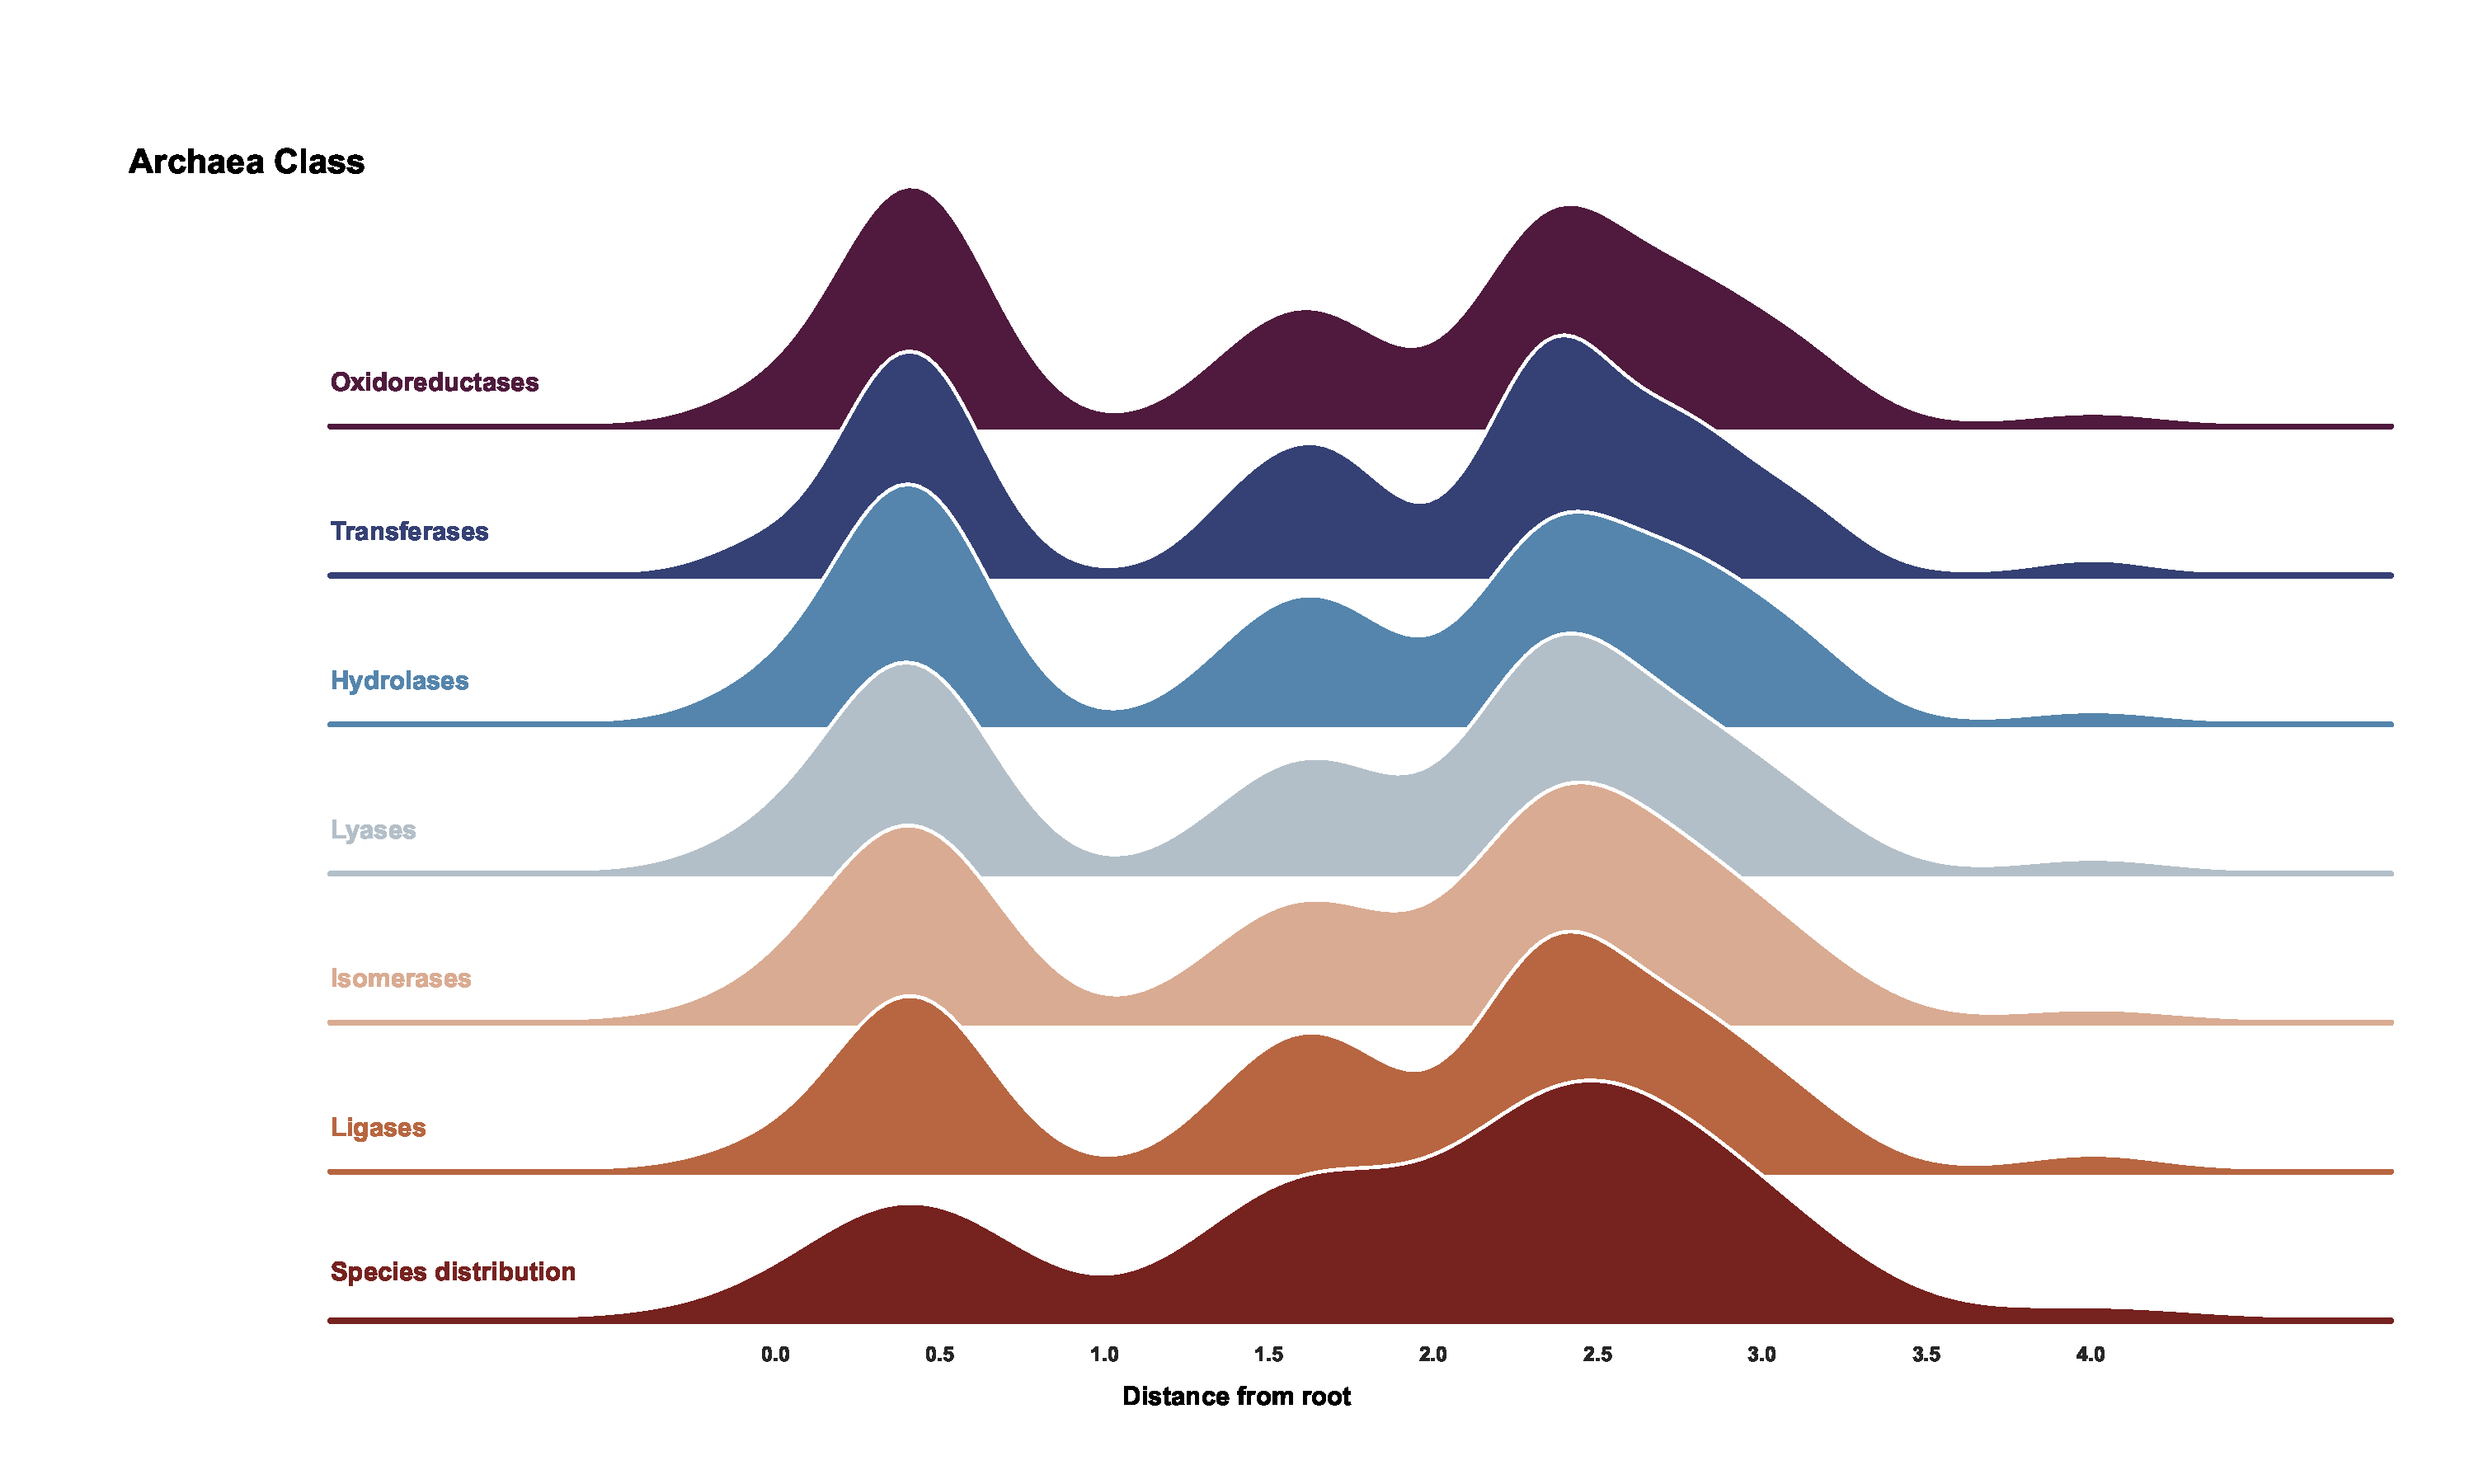
\includegraphics[width=0.95\textwidth]{ridgeplots/cla4arc_ridgeplot.pdf}
    \label{ridgeplot_cla4arc}
\end{figure}

\begin{figure}[H]
    \centering
    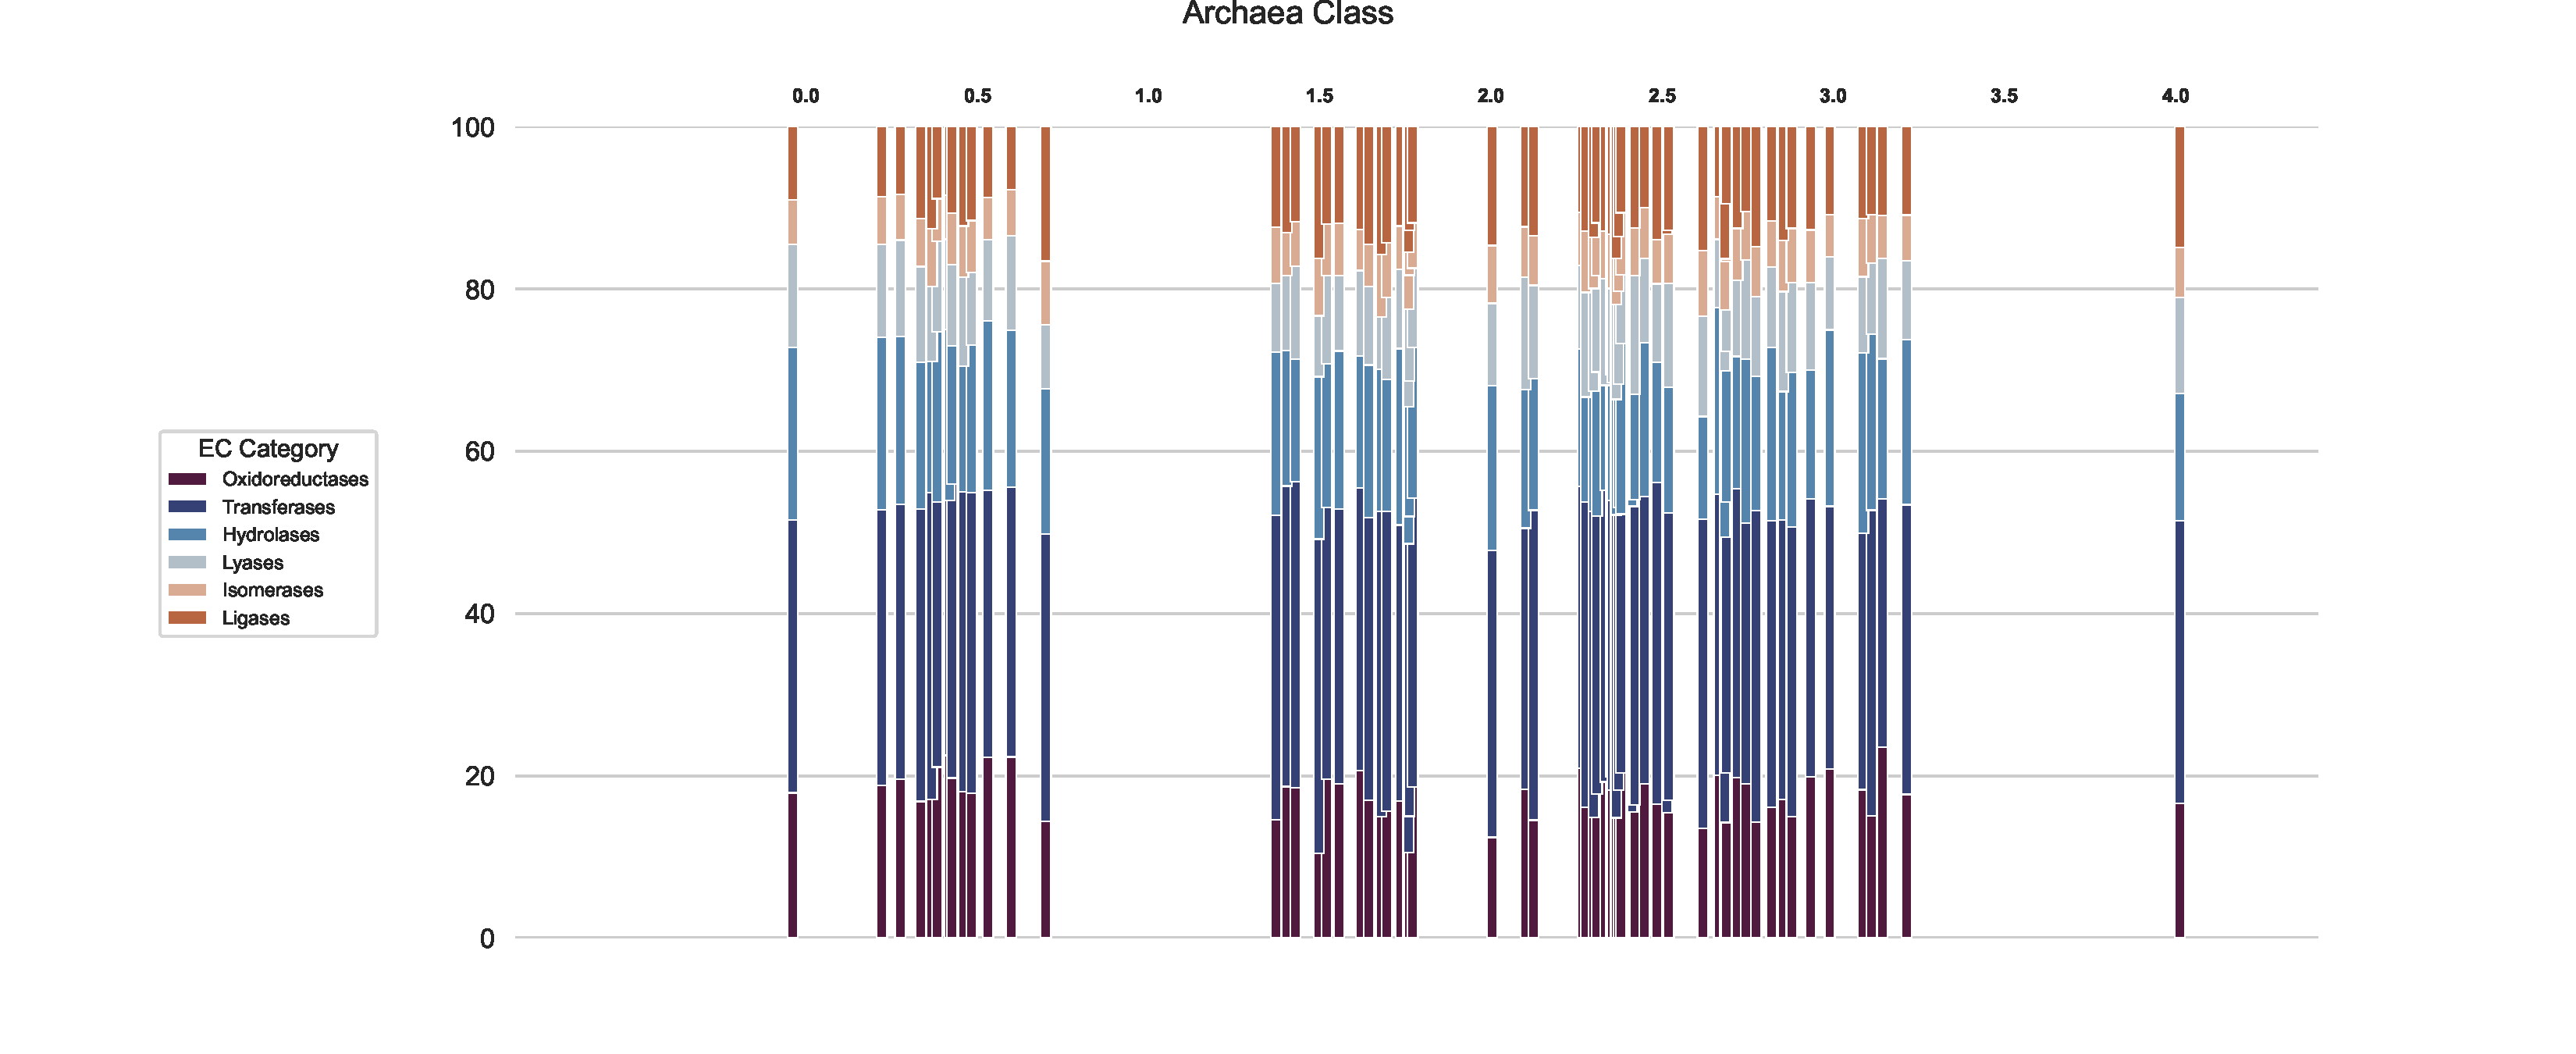
\includegraphics[width=0.95\textwidth]{ridgeplots/cla4arc_barplot.pdf}
    \caption[]{Class level archaea}
    \label{barplot_cla4arc}
\end{figure}

\begin{figure}[H]
    \centering
    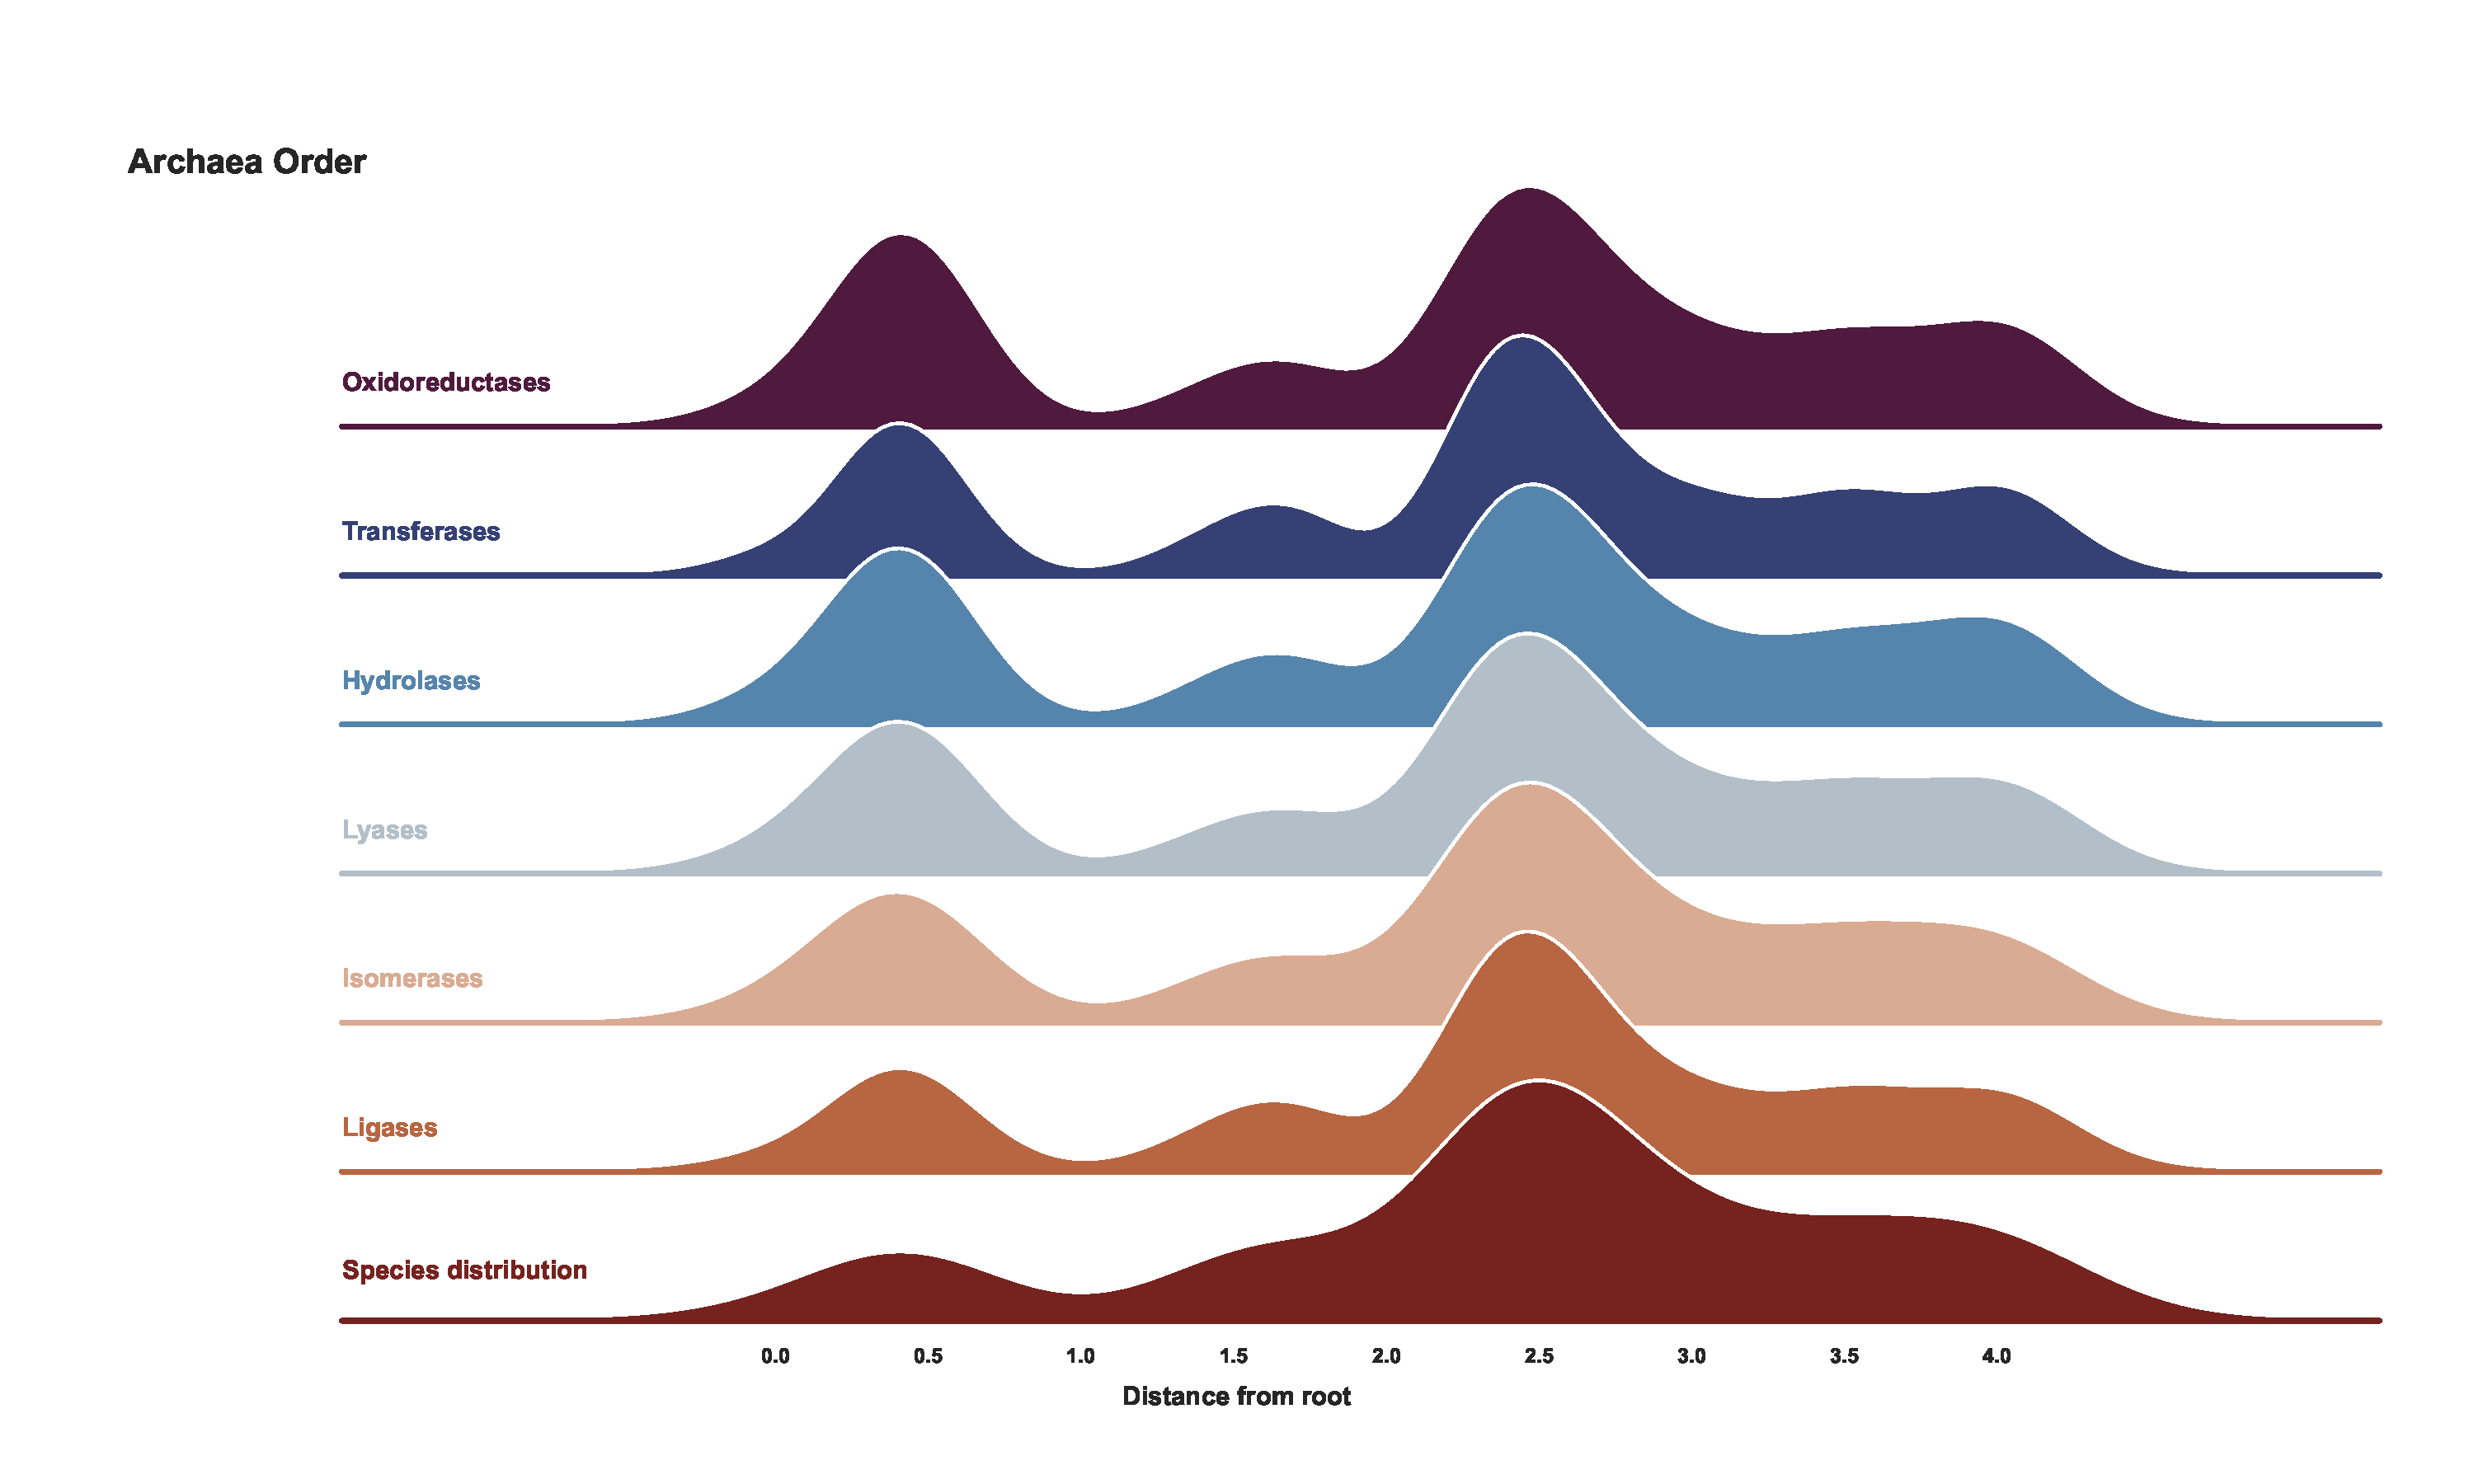
\includegraphics[width=0.95\textwidth]{ridgeplots/ord4arc_ridgeplot.pdf}
    \label{ridgeplot_ord4arc}
\end{figure}

\begin{figure}[H]
    \centering
    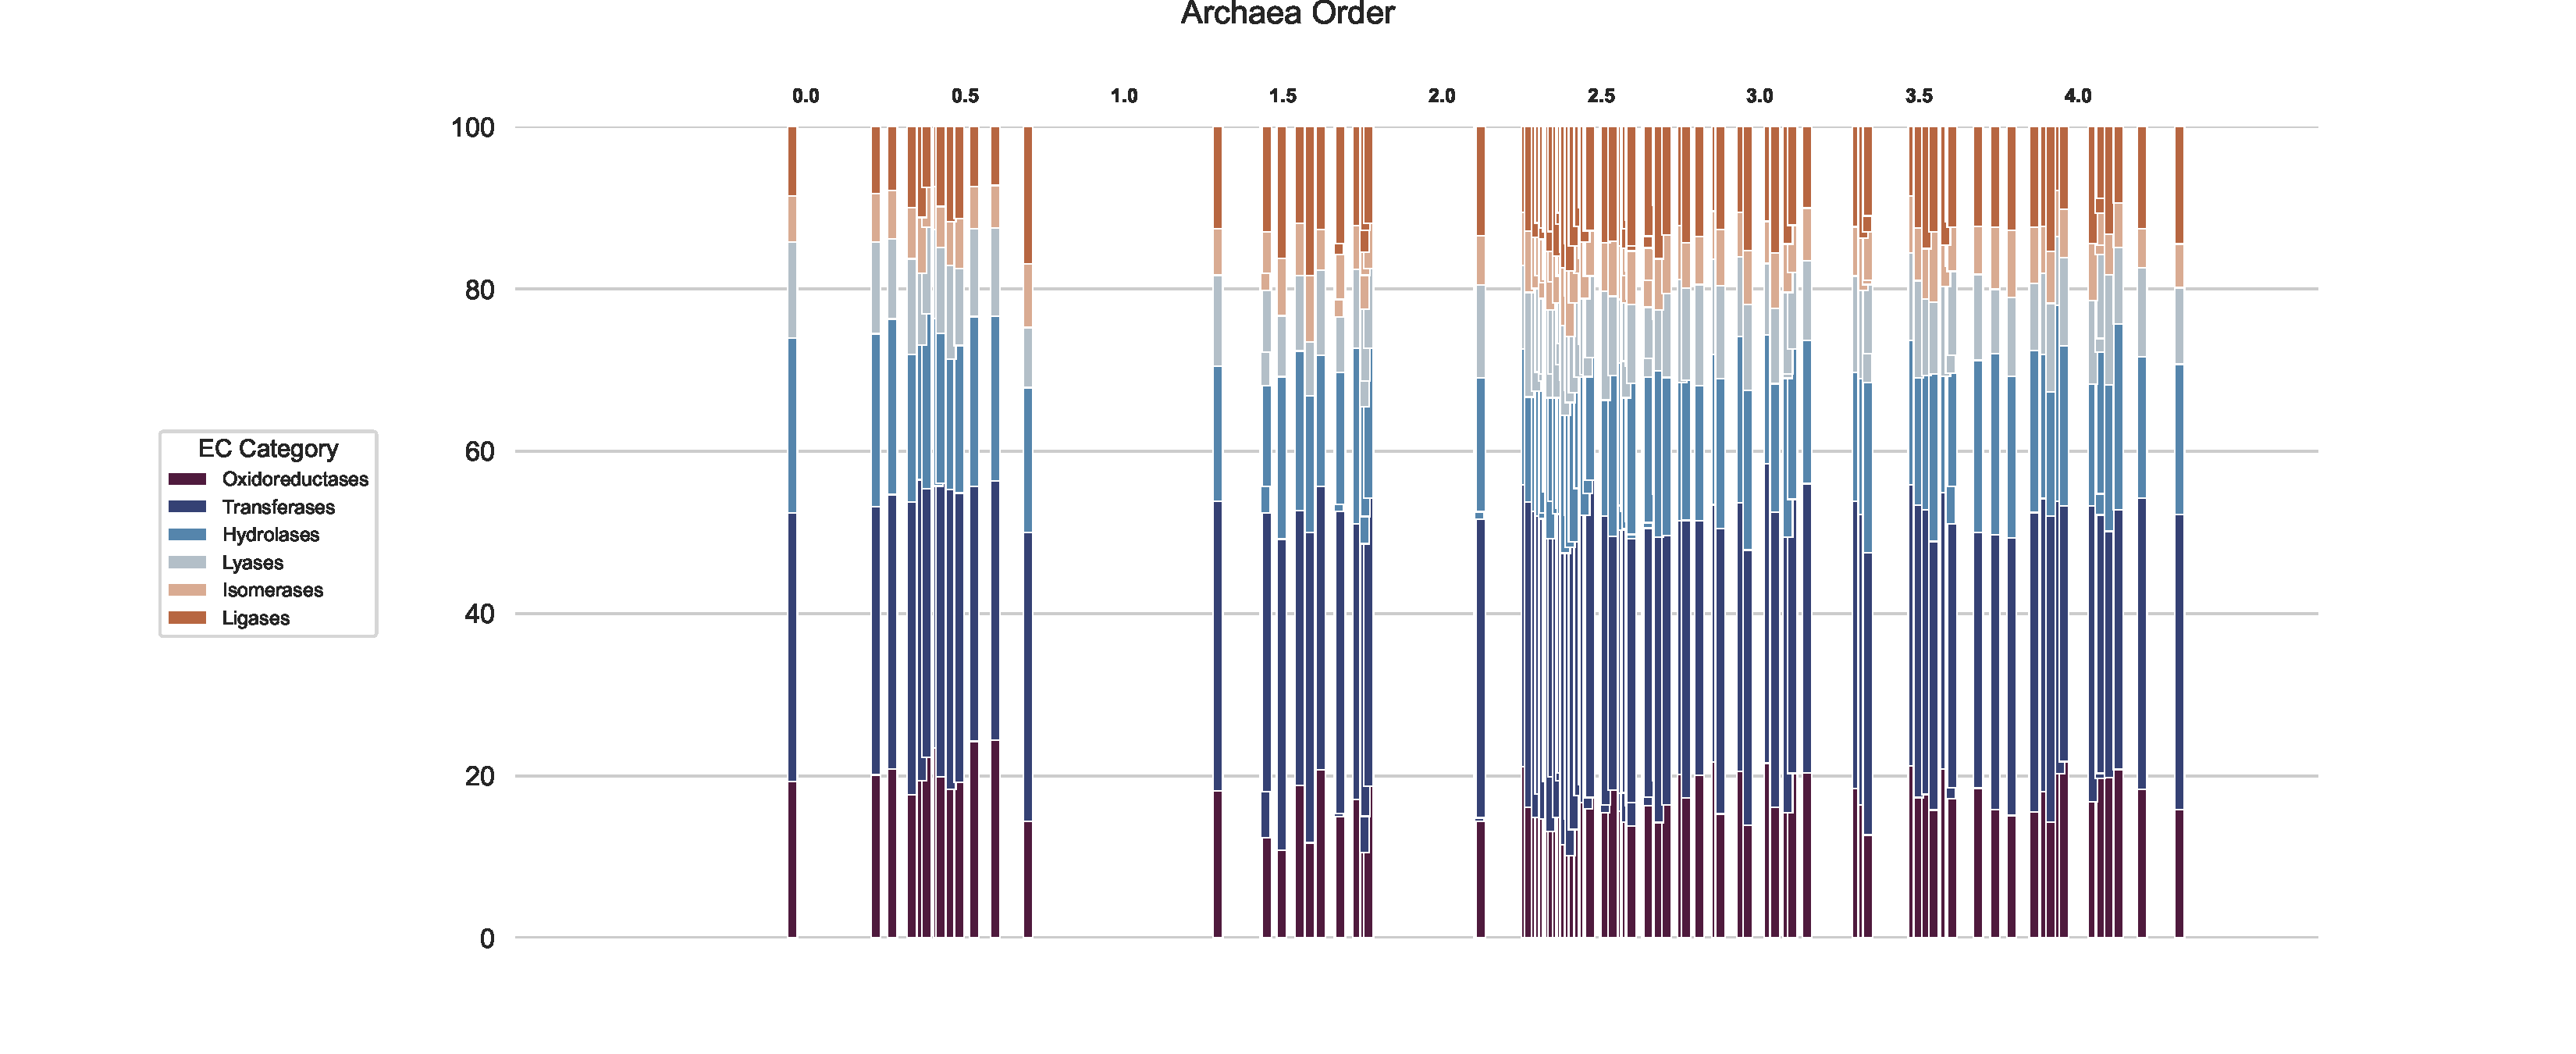
\includegraphics[width=0.95\textwidth]{ridgeplots/ord4arc_barplot.pdf}
    \caption[]{Order level archaea}
    \label{barplot_ord4arc}
\end{figure}

\begin{figure}[H]
    \centering
    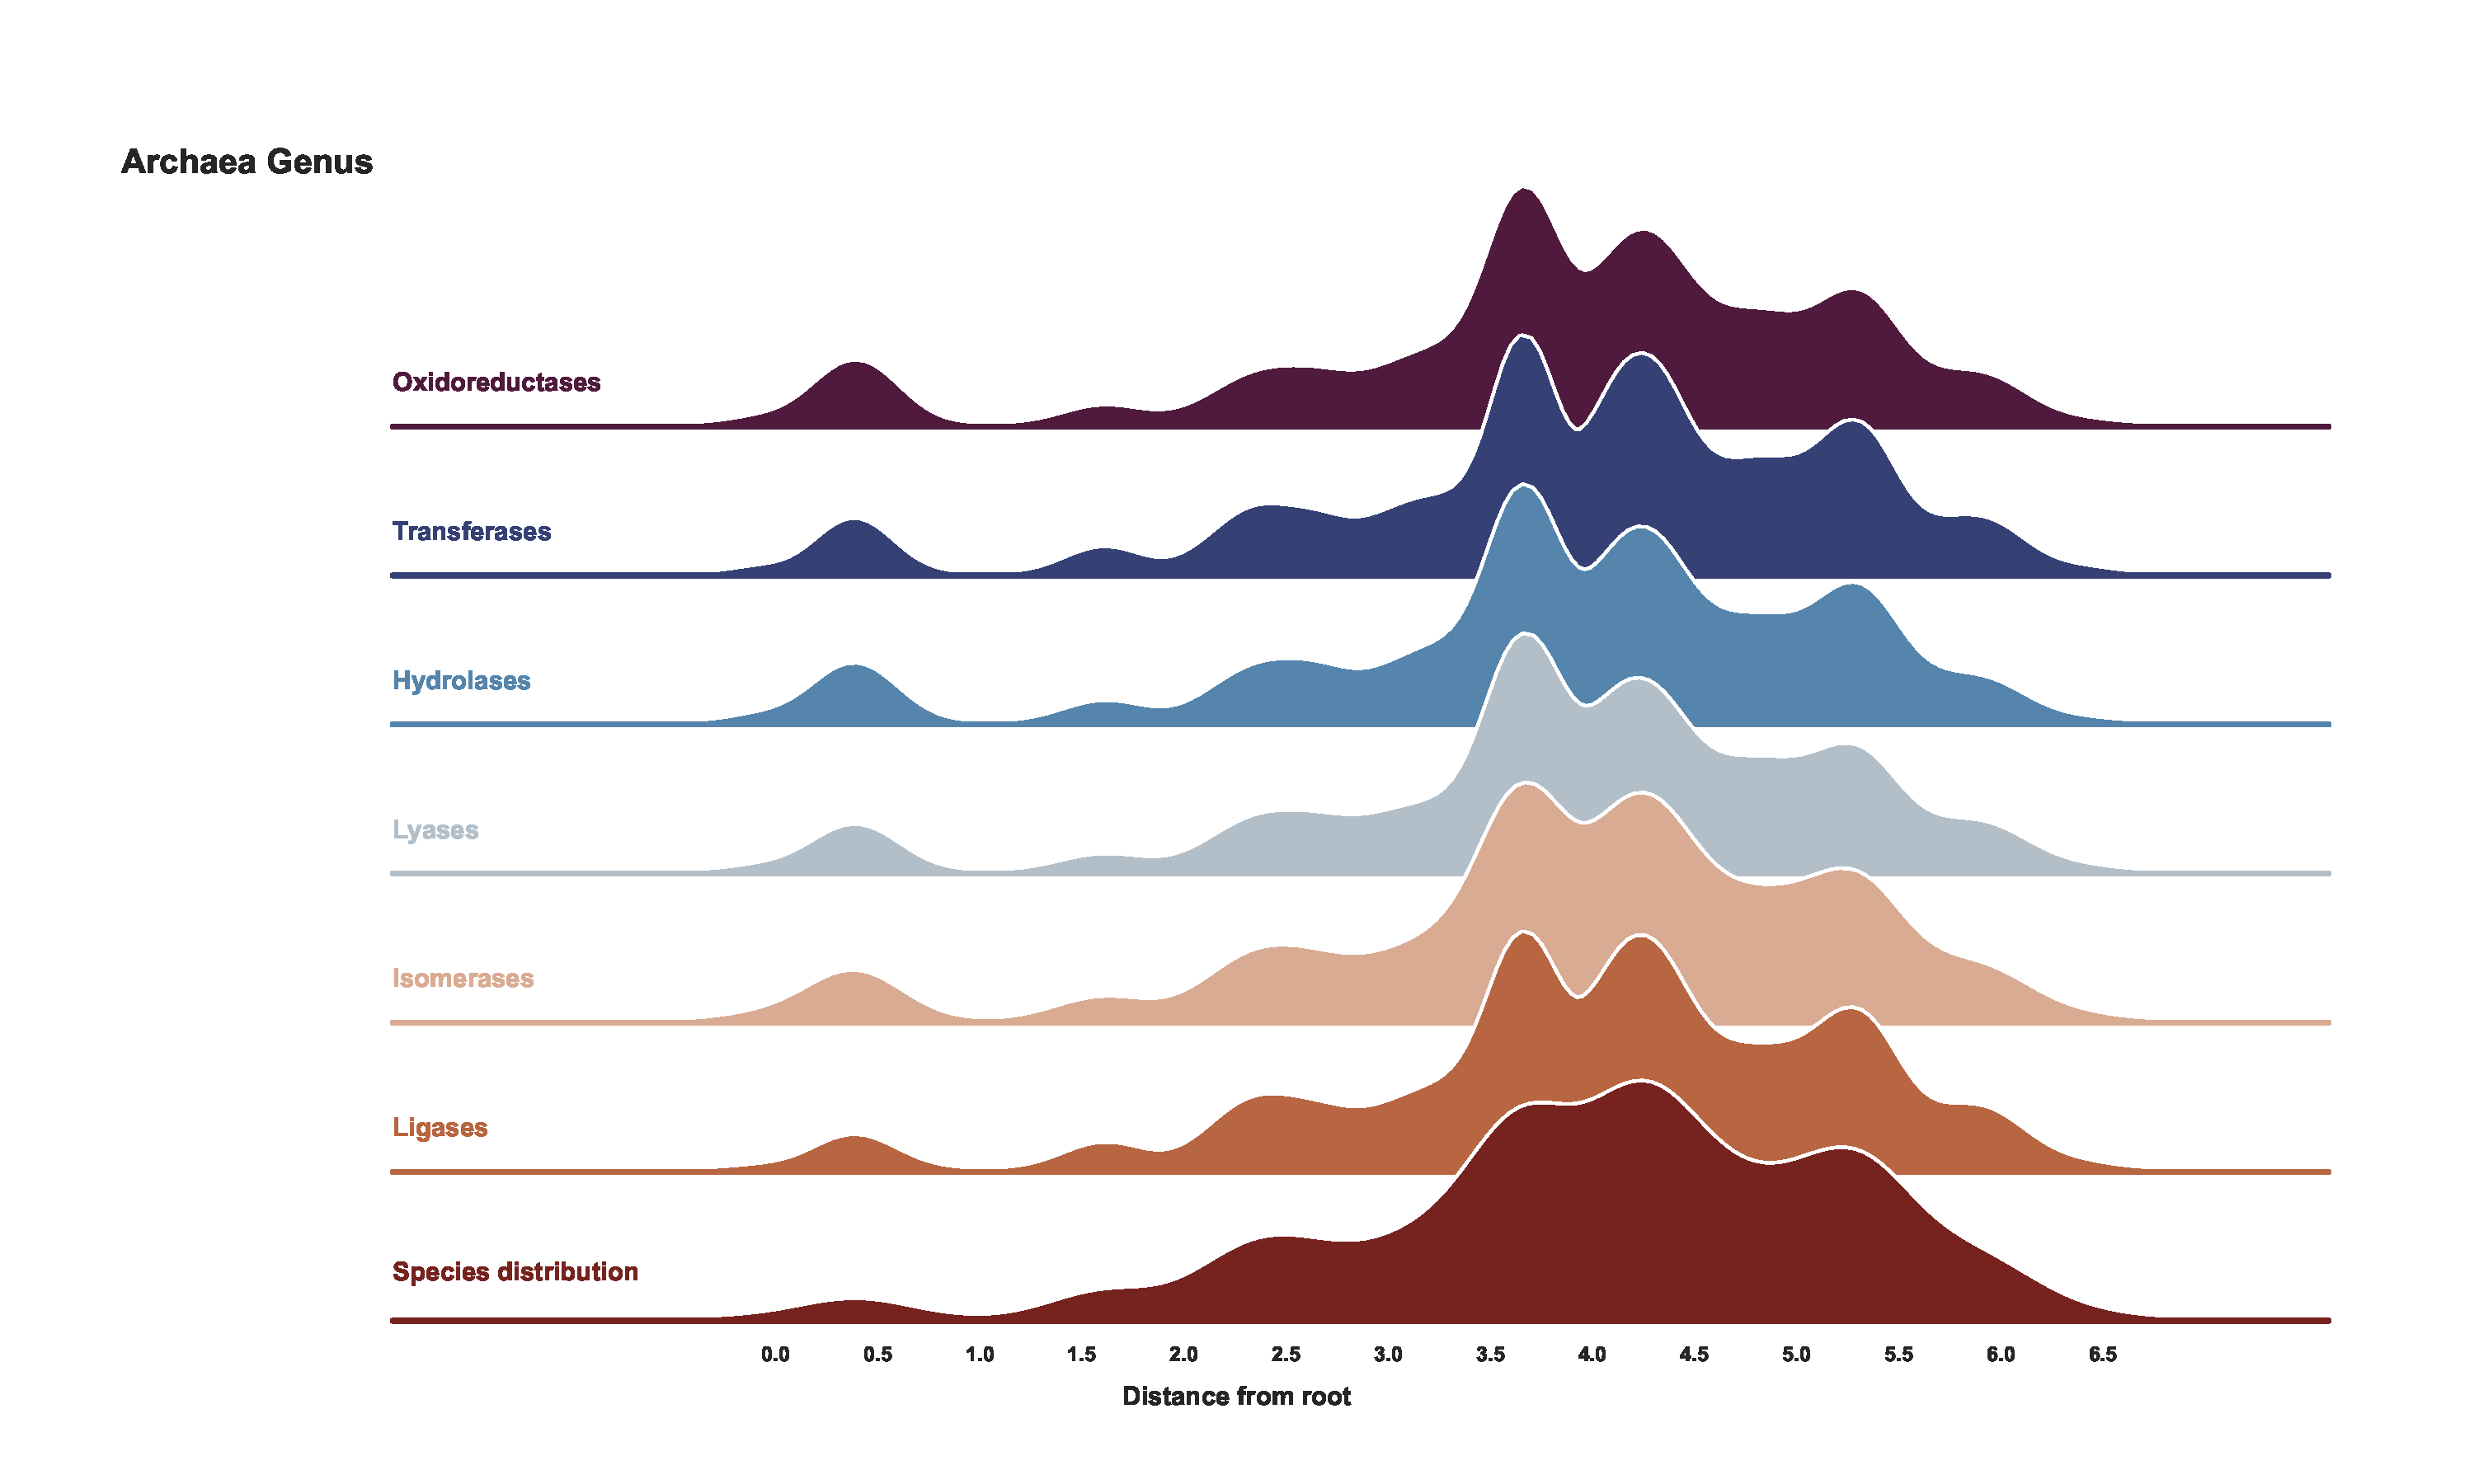
\includegraphics[width=0.95\textwidth]{ridgeplots/gen4arc_ridgeplot.pdf}
    \label{ridgeplot_gen4arc}
\end{figure}

\begin{figure}[H]
    \centering
    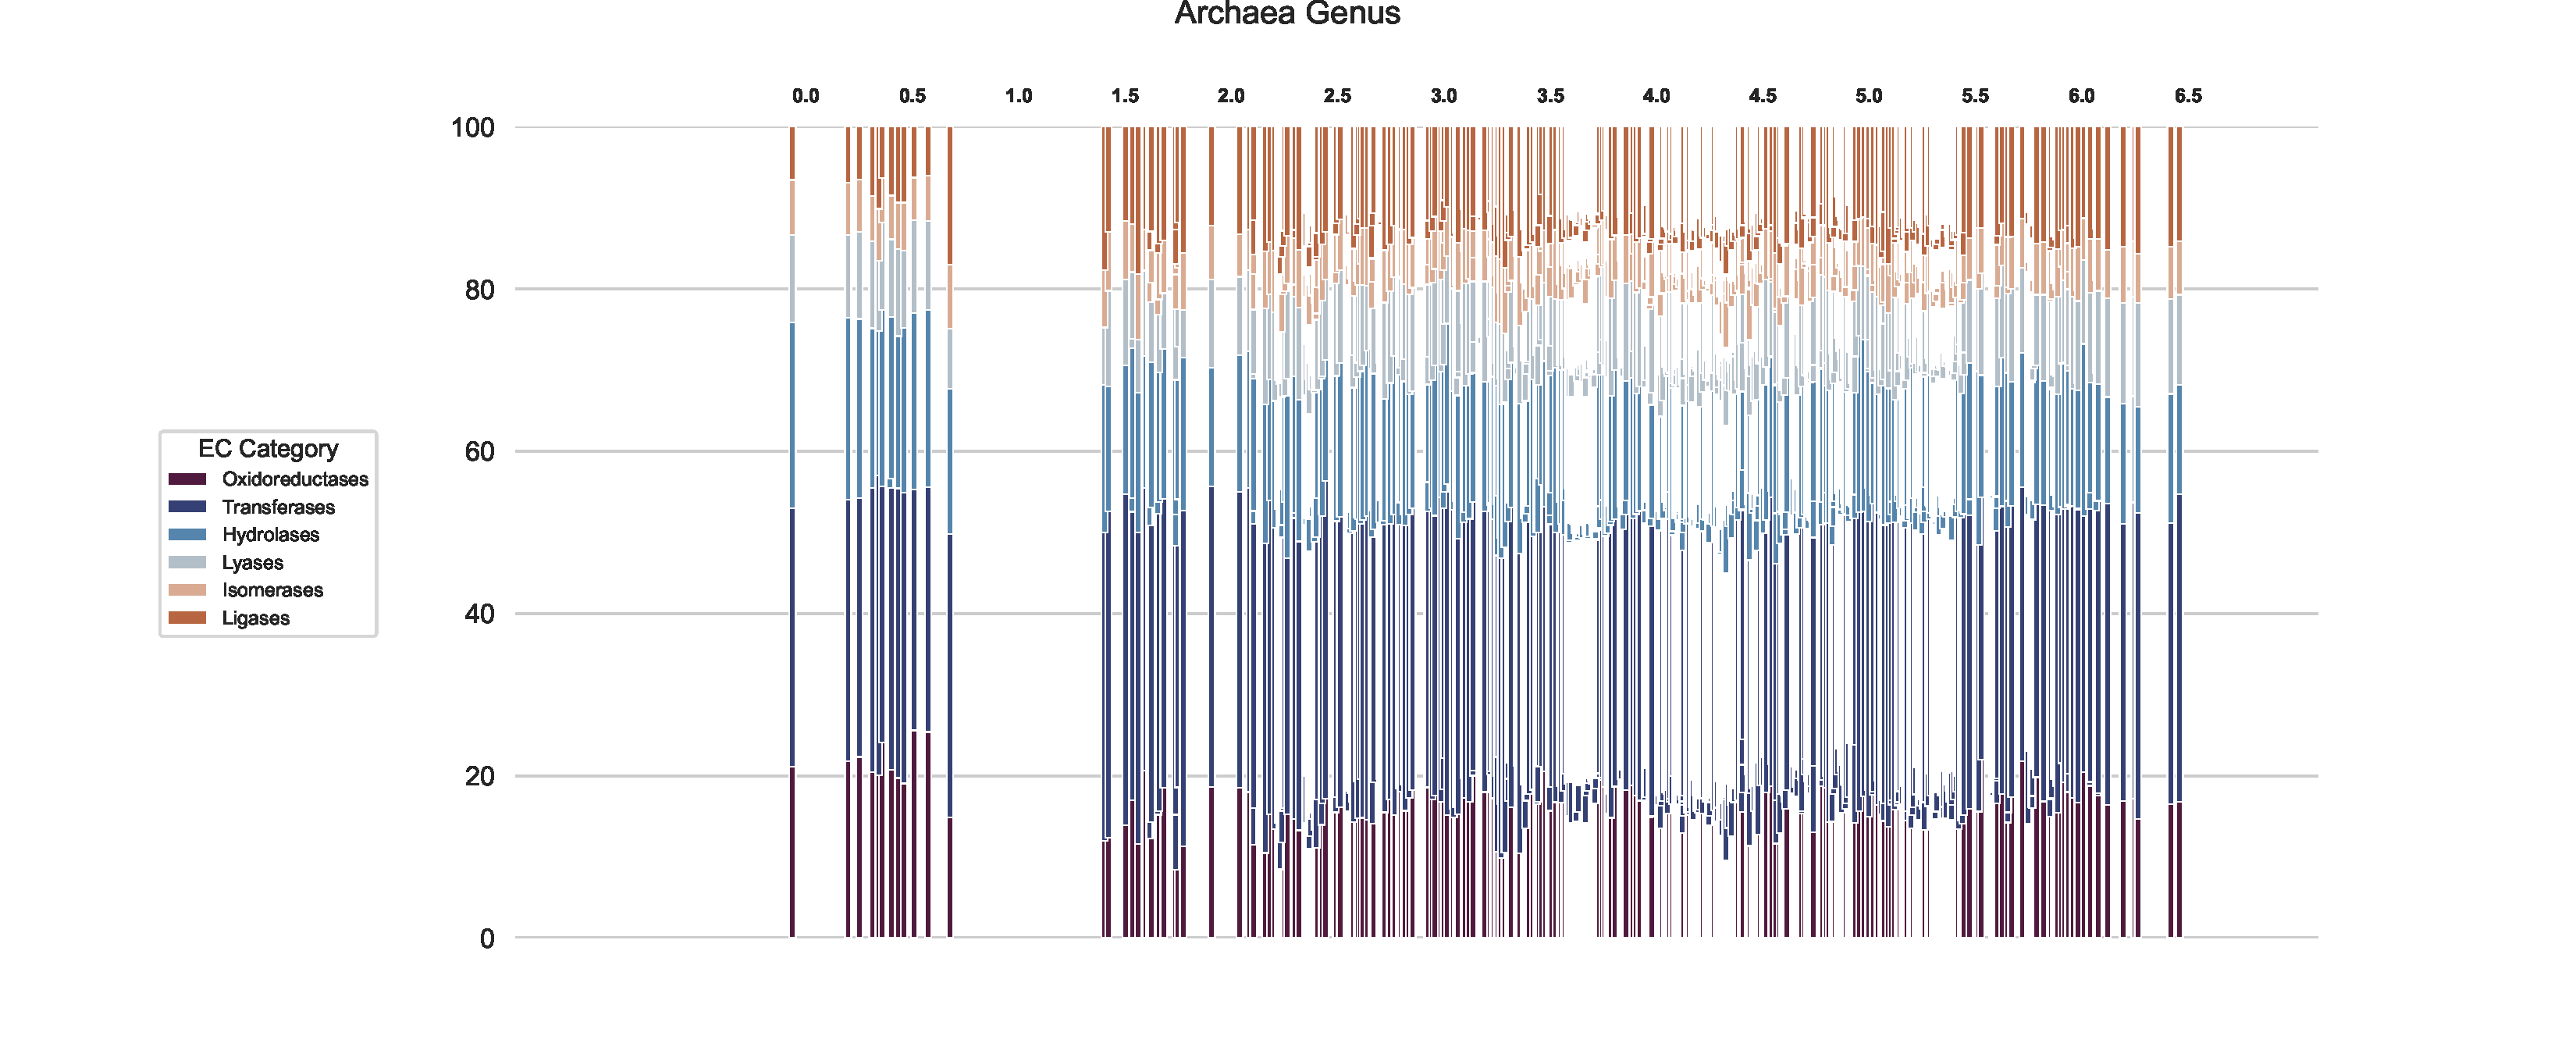
\includegraphics[width=0.95\textwidth]{ridgeplots/gen4arc_barplot.pdf}
    \caption[]{Genus level archaea}
    \label{barplot_gen4arc}
\end{figure}



\subsection*{A3. Expansion Scope Size as a Function of Distance to Root}
\textbf{For every taxonomic level dataset, per seed set.}

\begin{figure}[H]
    \centering
    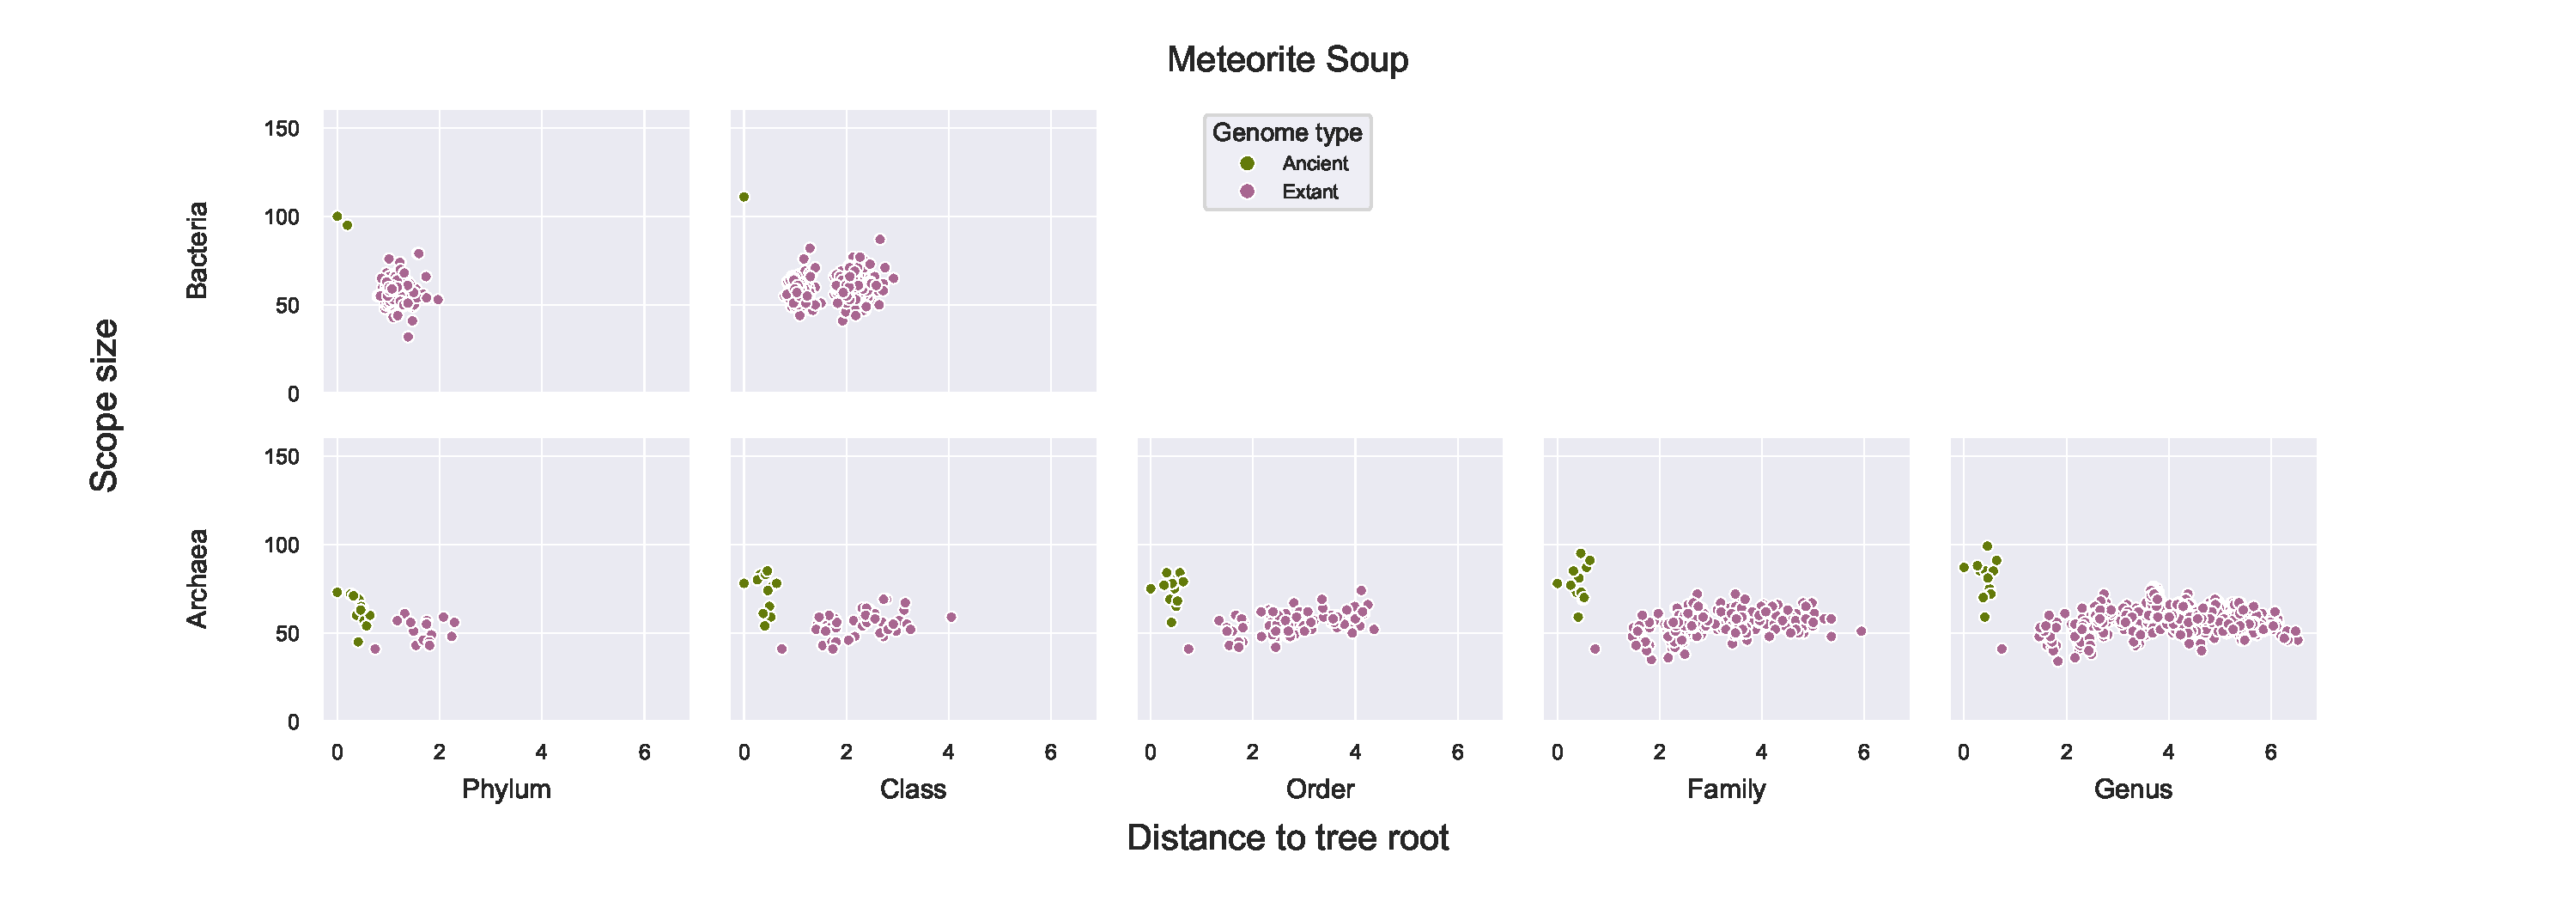
\includegraphics[width=0.95\textwidth]{scopesize_vs_disttoroot/gfm_ss_rootdist}
    \caption{Goldford + meteoritic soup}
    \label{gfm_scopesize}
\end{figure}   

\begin{figure}[H]
    \centering
    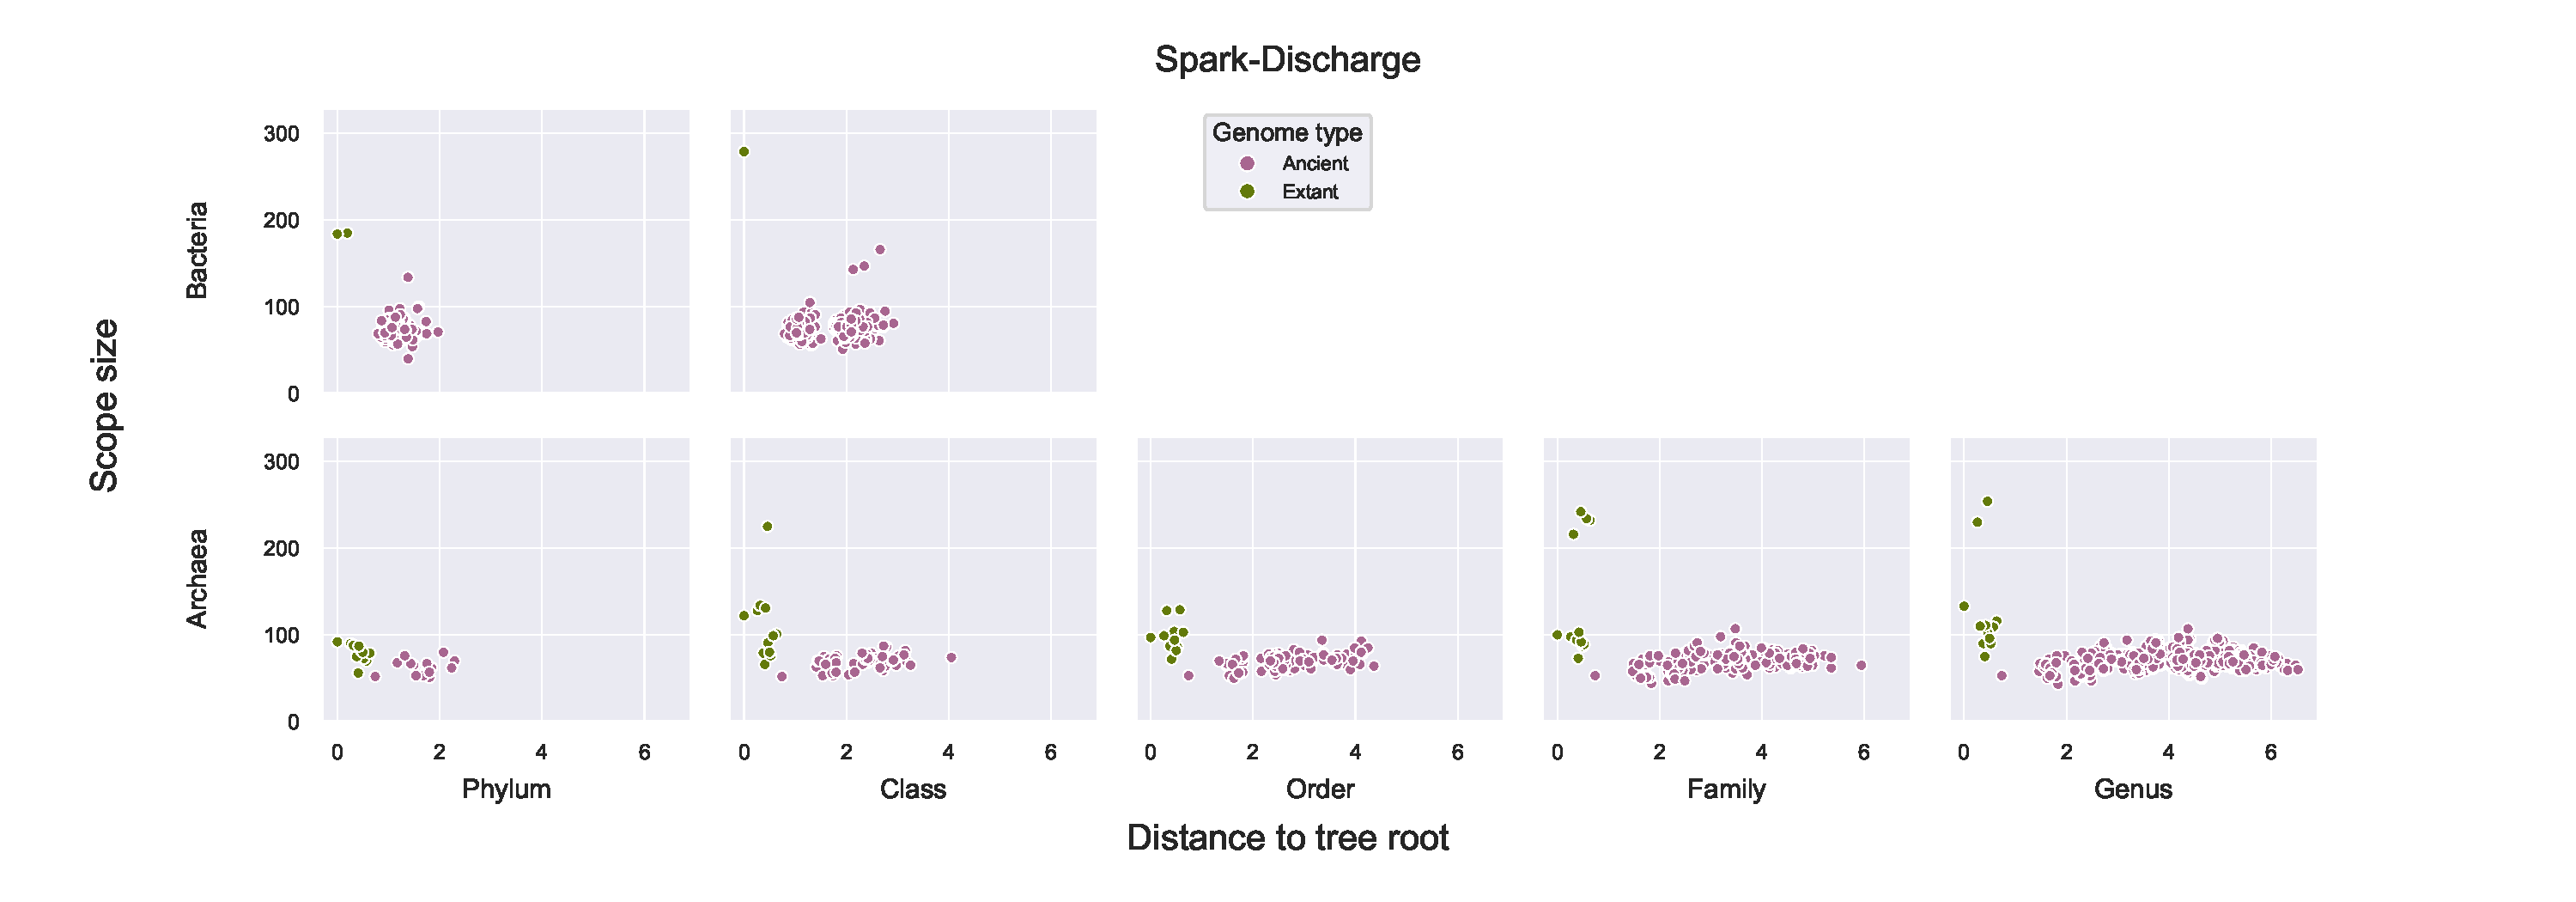
\includegraphics[width=0.95\textwidth]{scopesize_vs_disttoroot/gfsd_ss_rootdist.pdf}
    \caption{Goldford + spark-discharge}
    \label{gfsd_scopesize}
\end{figure}   

\begin{figure}[H]
    \centering
    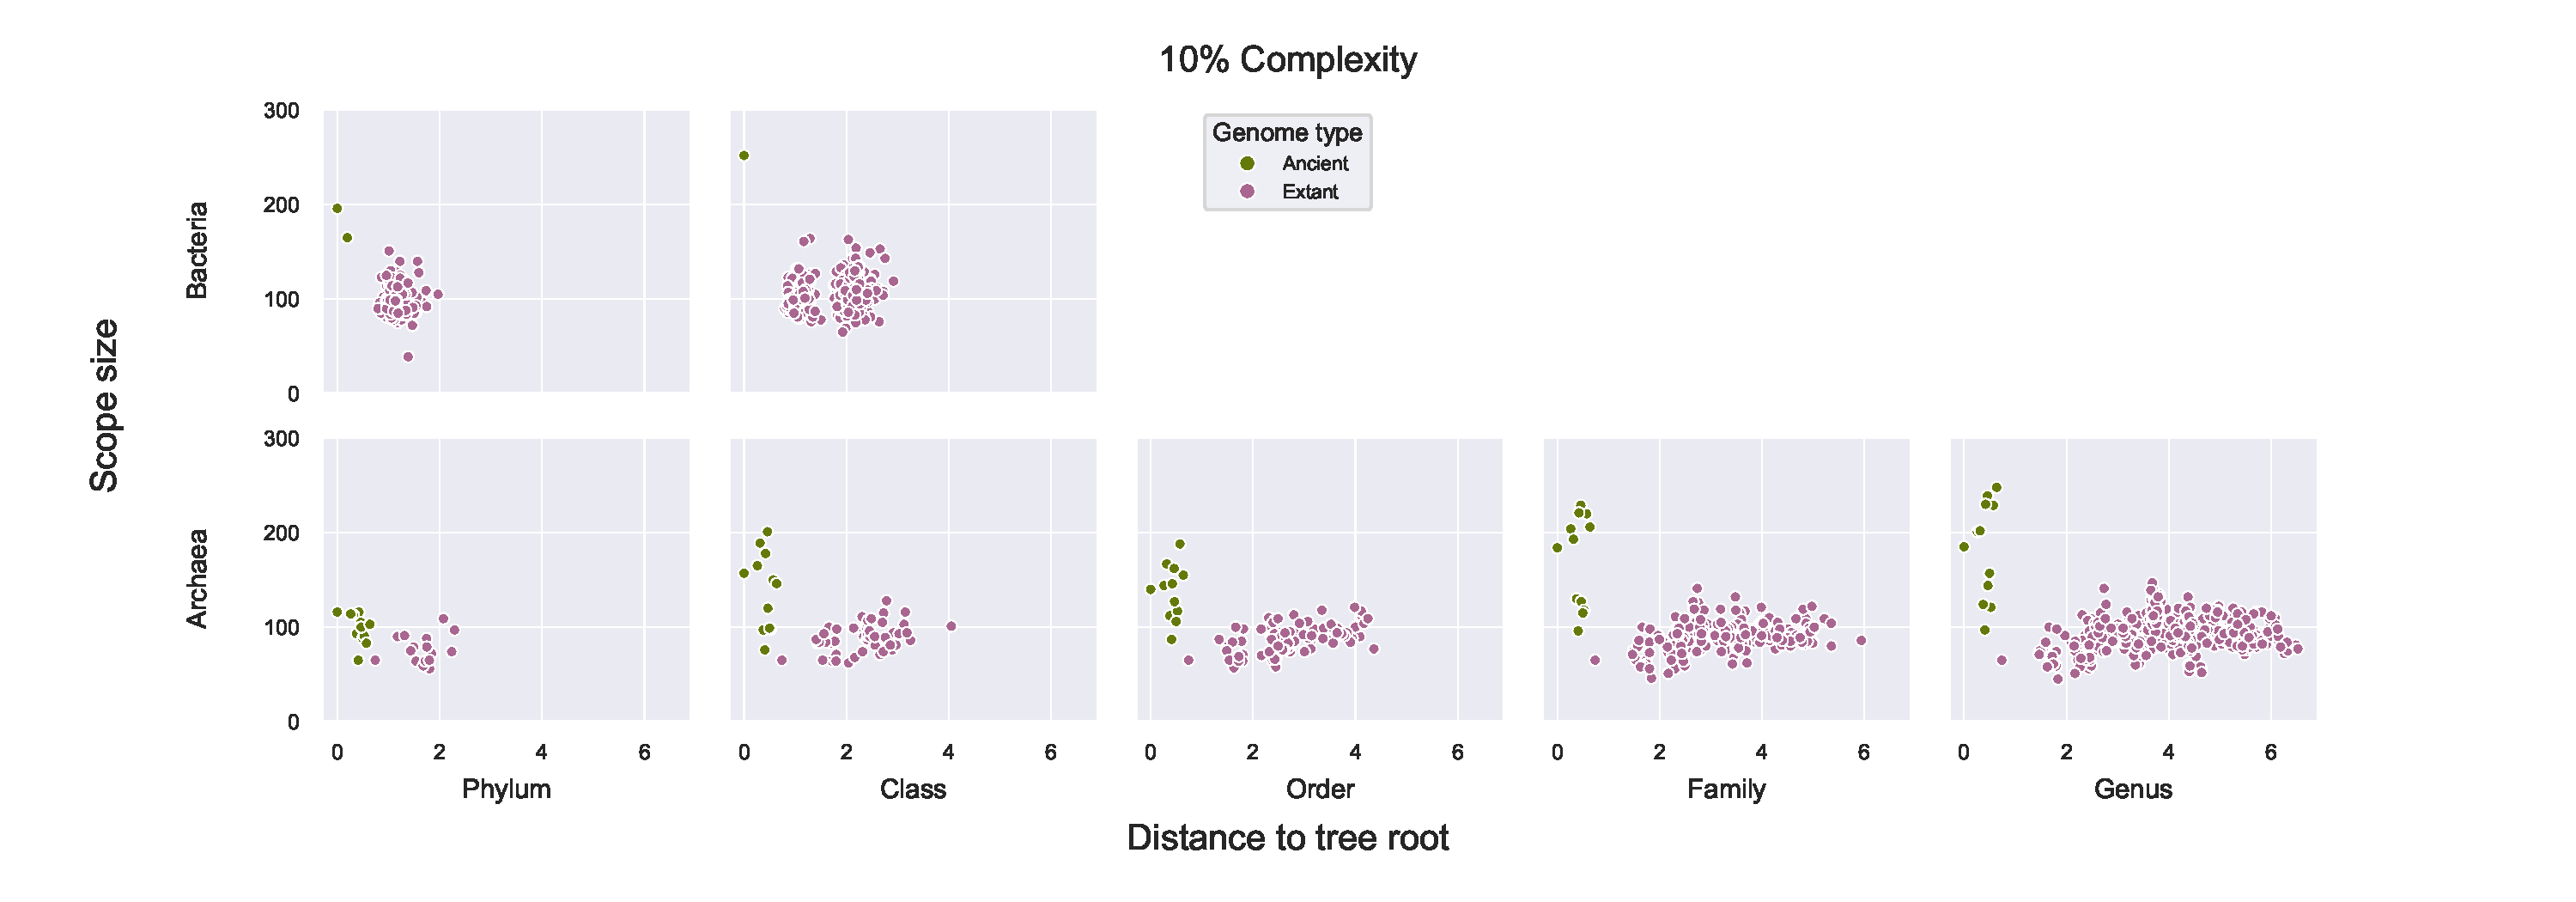
\includegraphics[width=0.95\textwidth]{scopesize_vs_disttoroot/0.1_ss_rootdist.pdf}
    \caption{10\% complexity}
    \label{0.1_scopesize}
\end{figure}   

\begin{figure}[H]
    \centering
    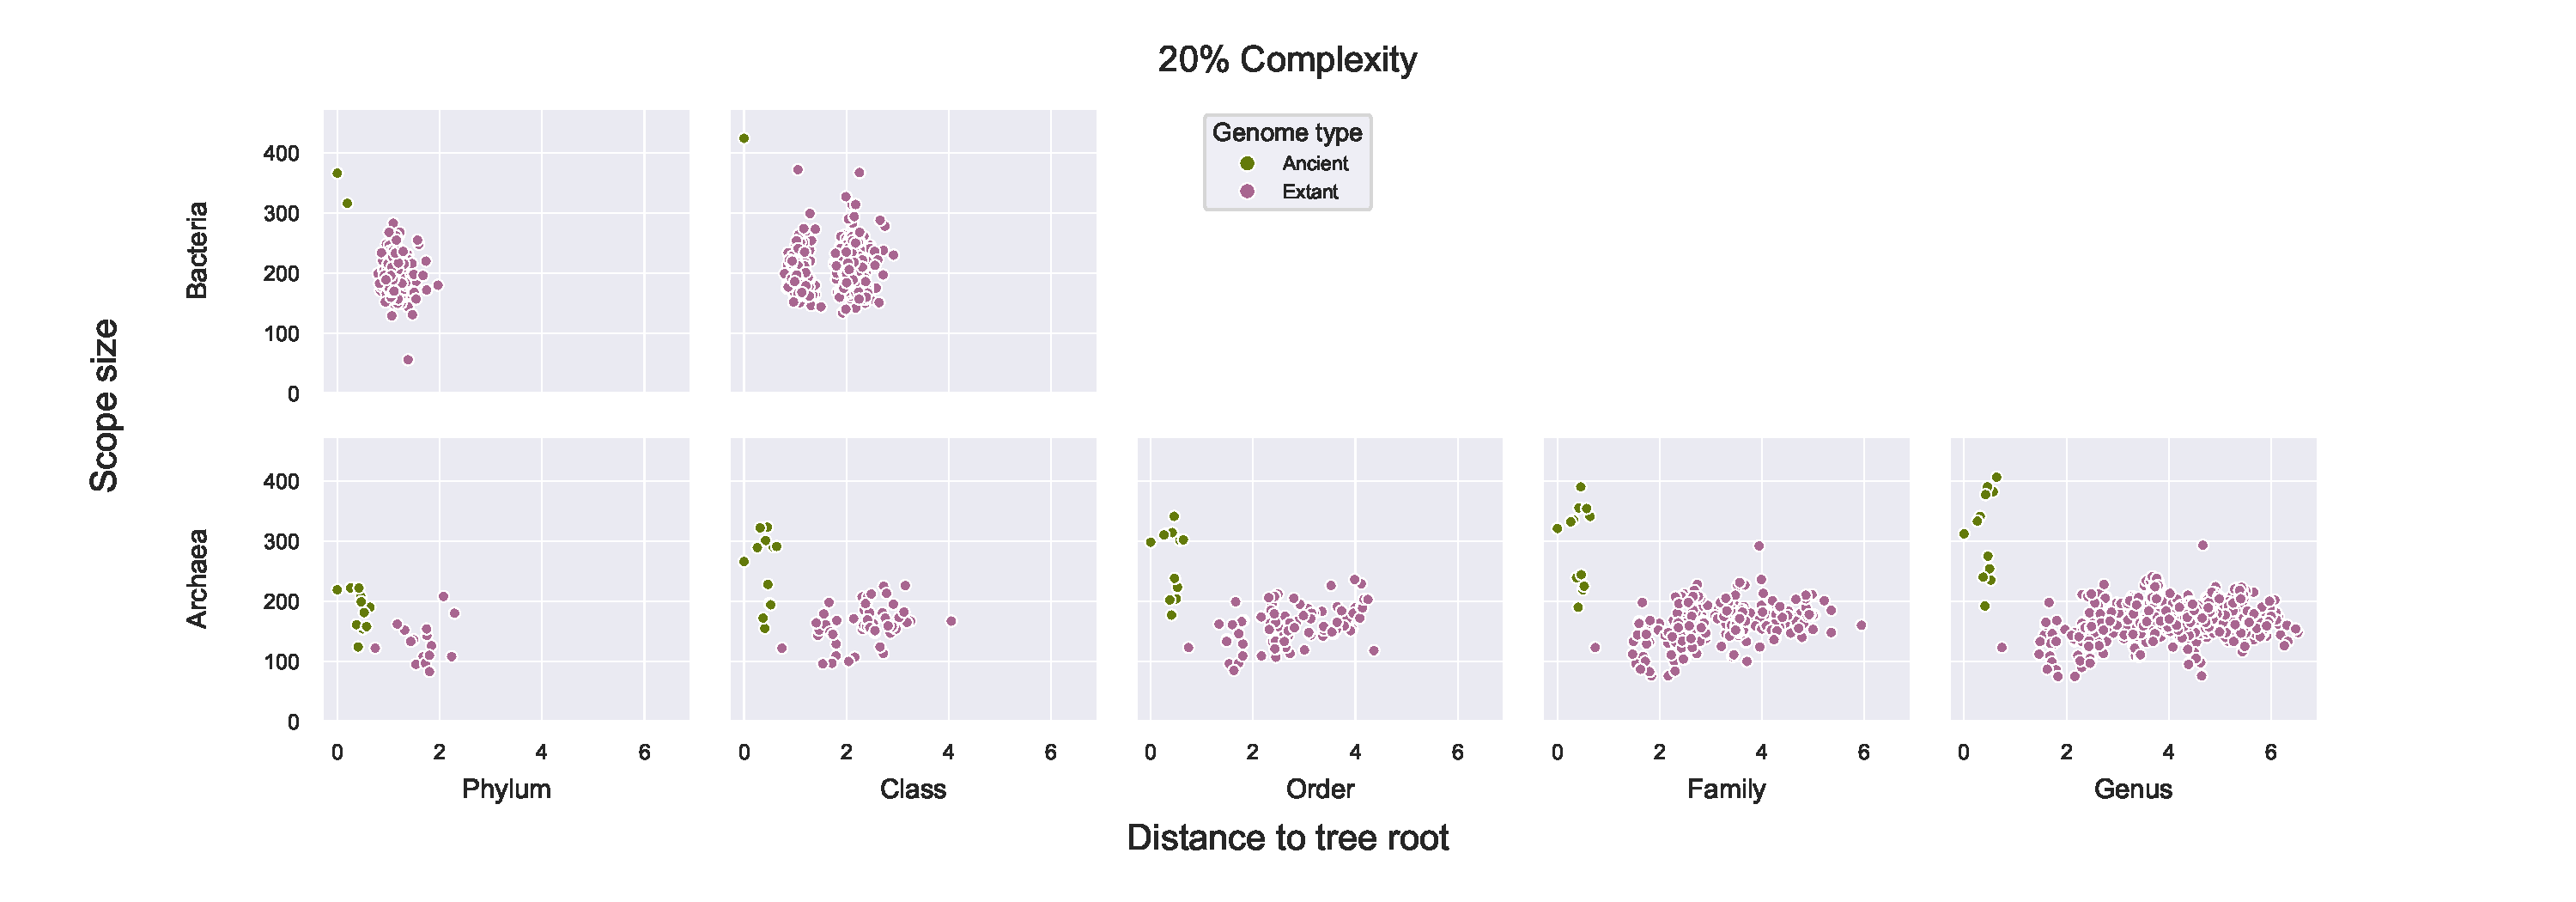
\includegraphics[width=0.95\textwidth]{scopesize_vs_disttoroot/0.2_ss_rootdist.pdf}
    \caption{20\% complexity}
    \label{0.2_scopesize}
\end{figure}   

\begin{figure}[H]
    \centering
    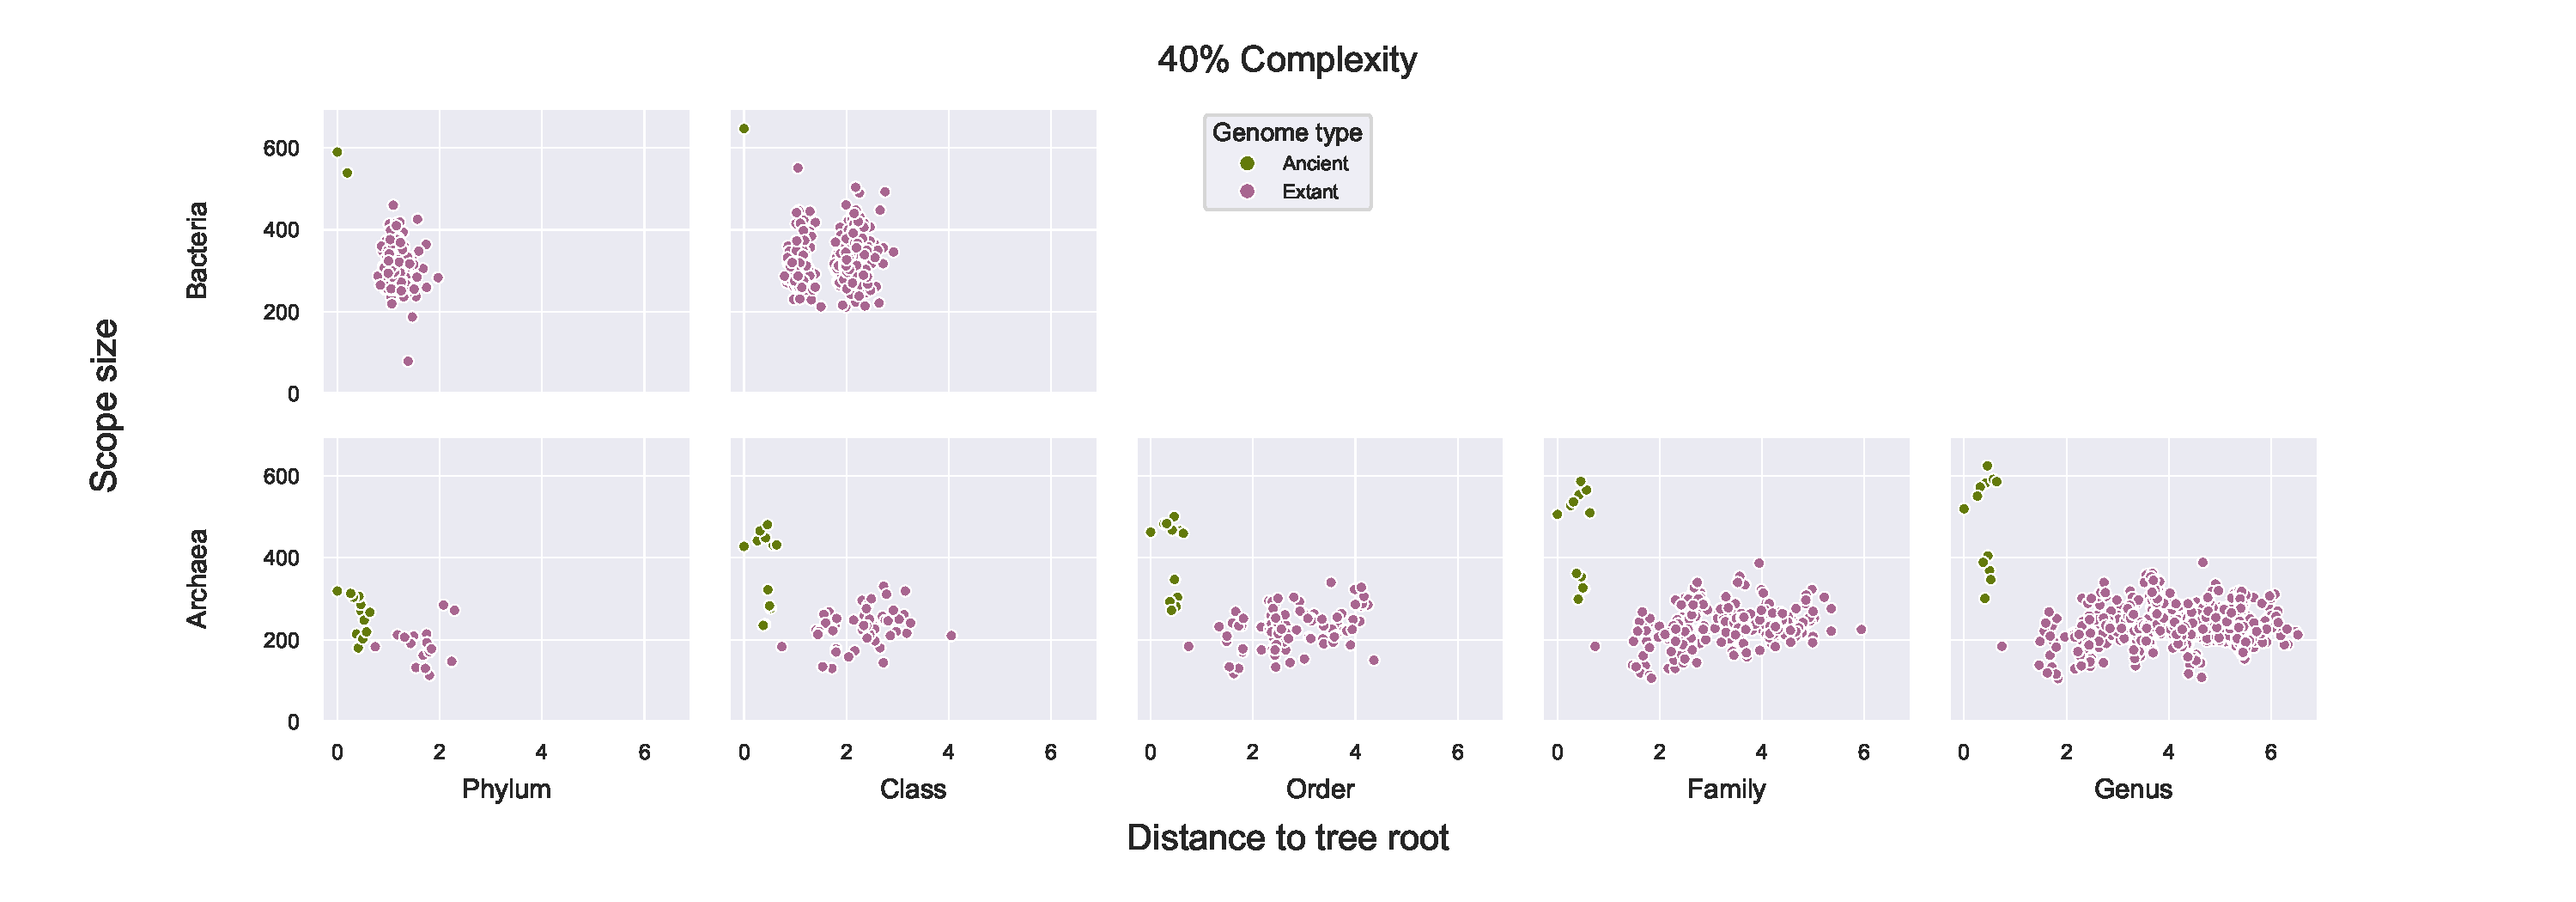
\includegraphics[width=0.95\textwidth]{scopesize_vs_disttoroot/0.4_ss_rootdist.pdf}
    \caption{40\% complexity}
    \label{0.4_scopesize}
\end{figure}   

\begin{figure}[H]
    \centering
    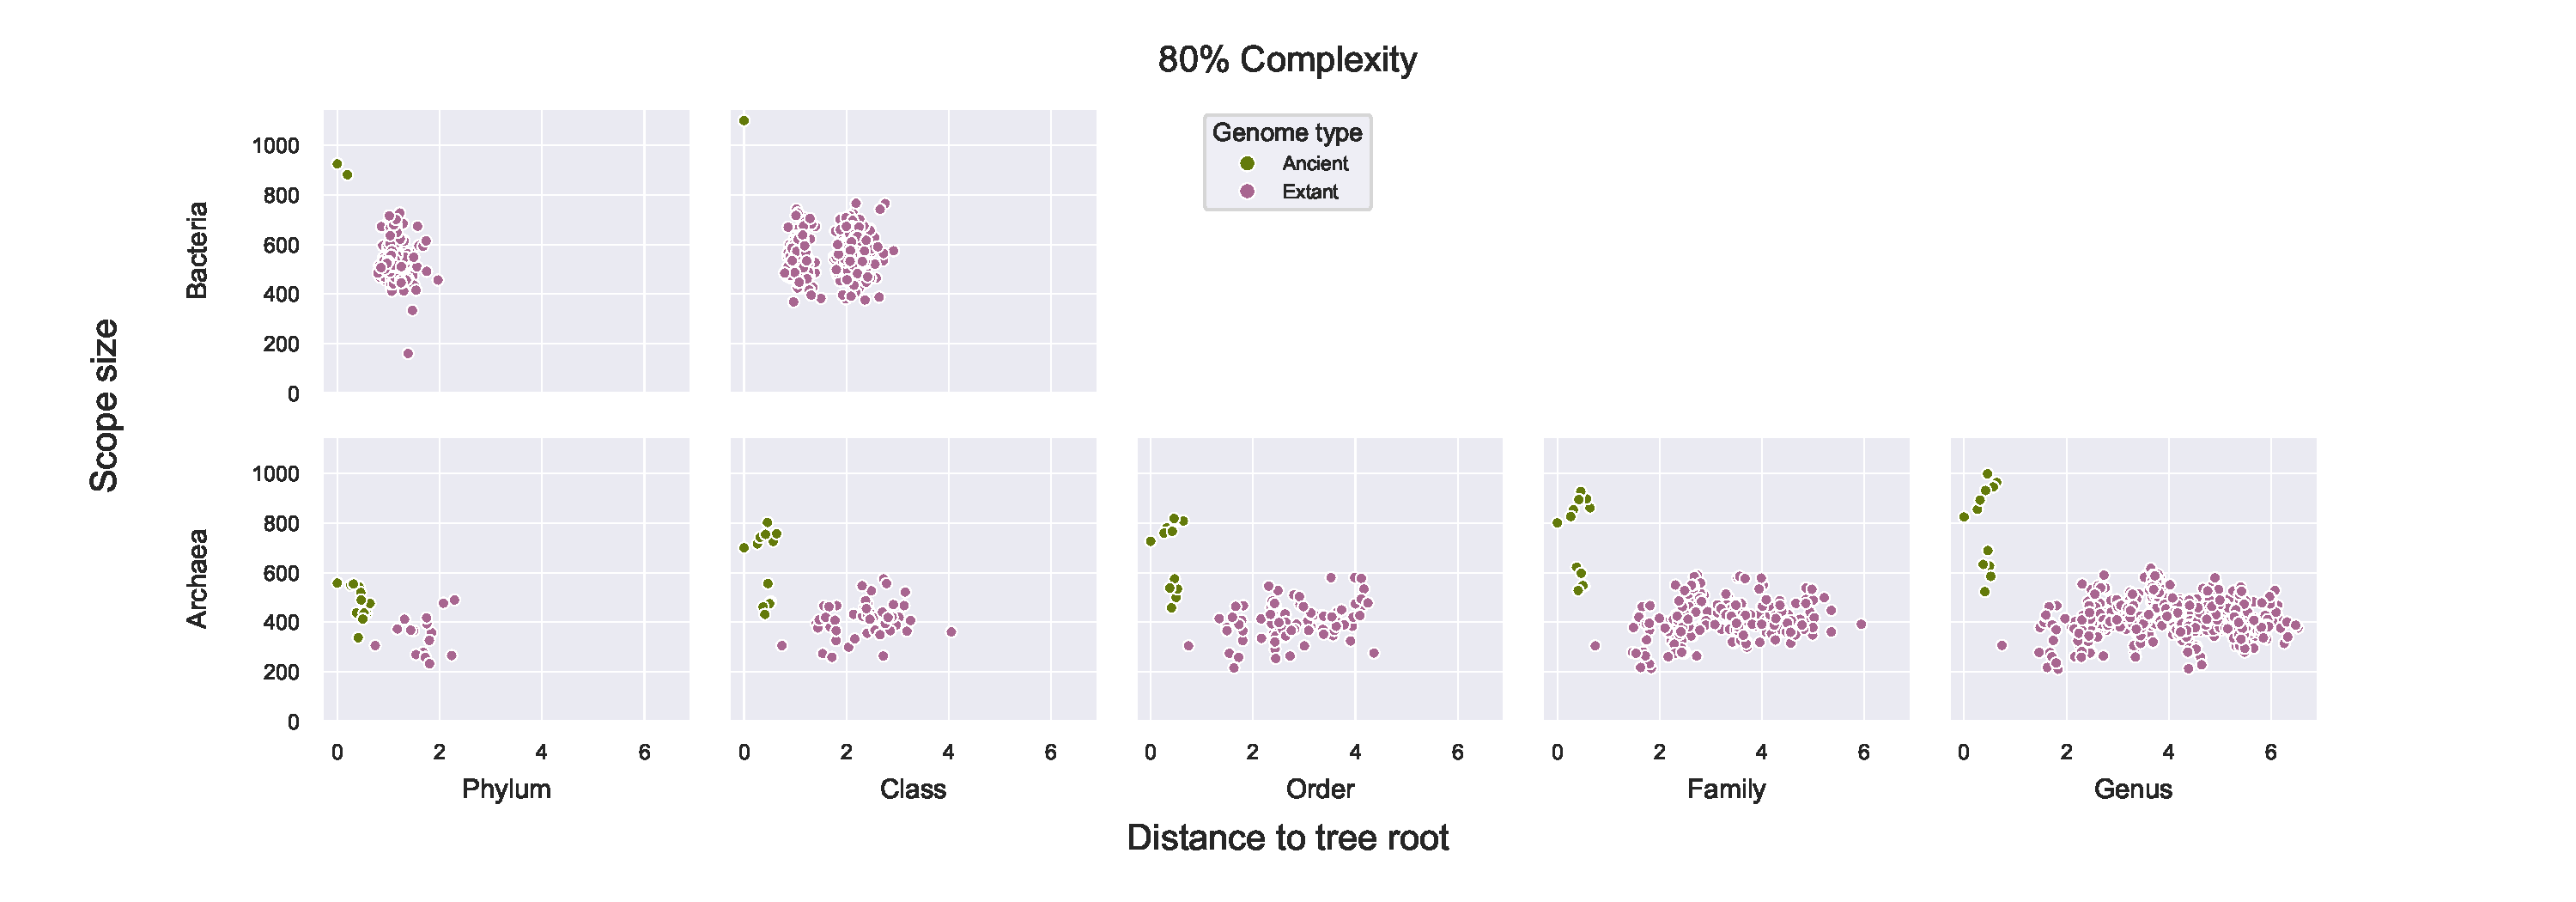
\includegraphics[width=0.95\textwidth]{scopesize_vs_disttoroot/0.8_ss_rootdist.pdf}
    \caption{80\% complexity}
    \label{0.8_scopesize}
\end{figure}   

\begin{figure}[H]
    \centering
    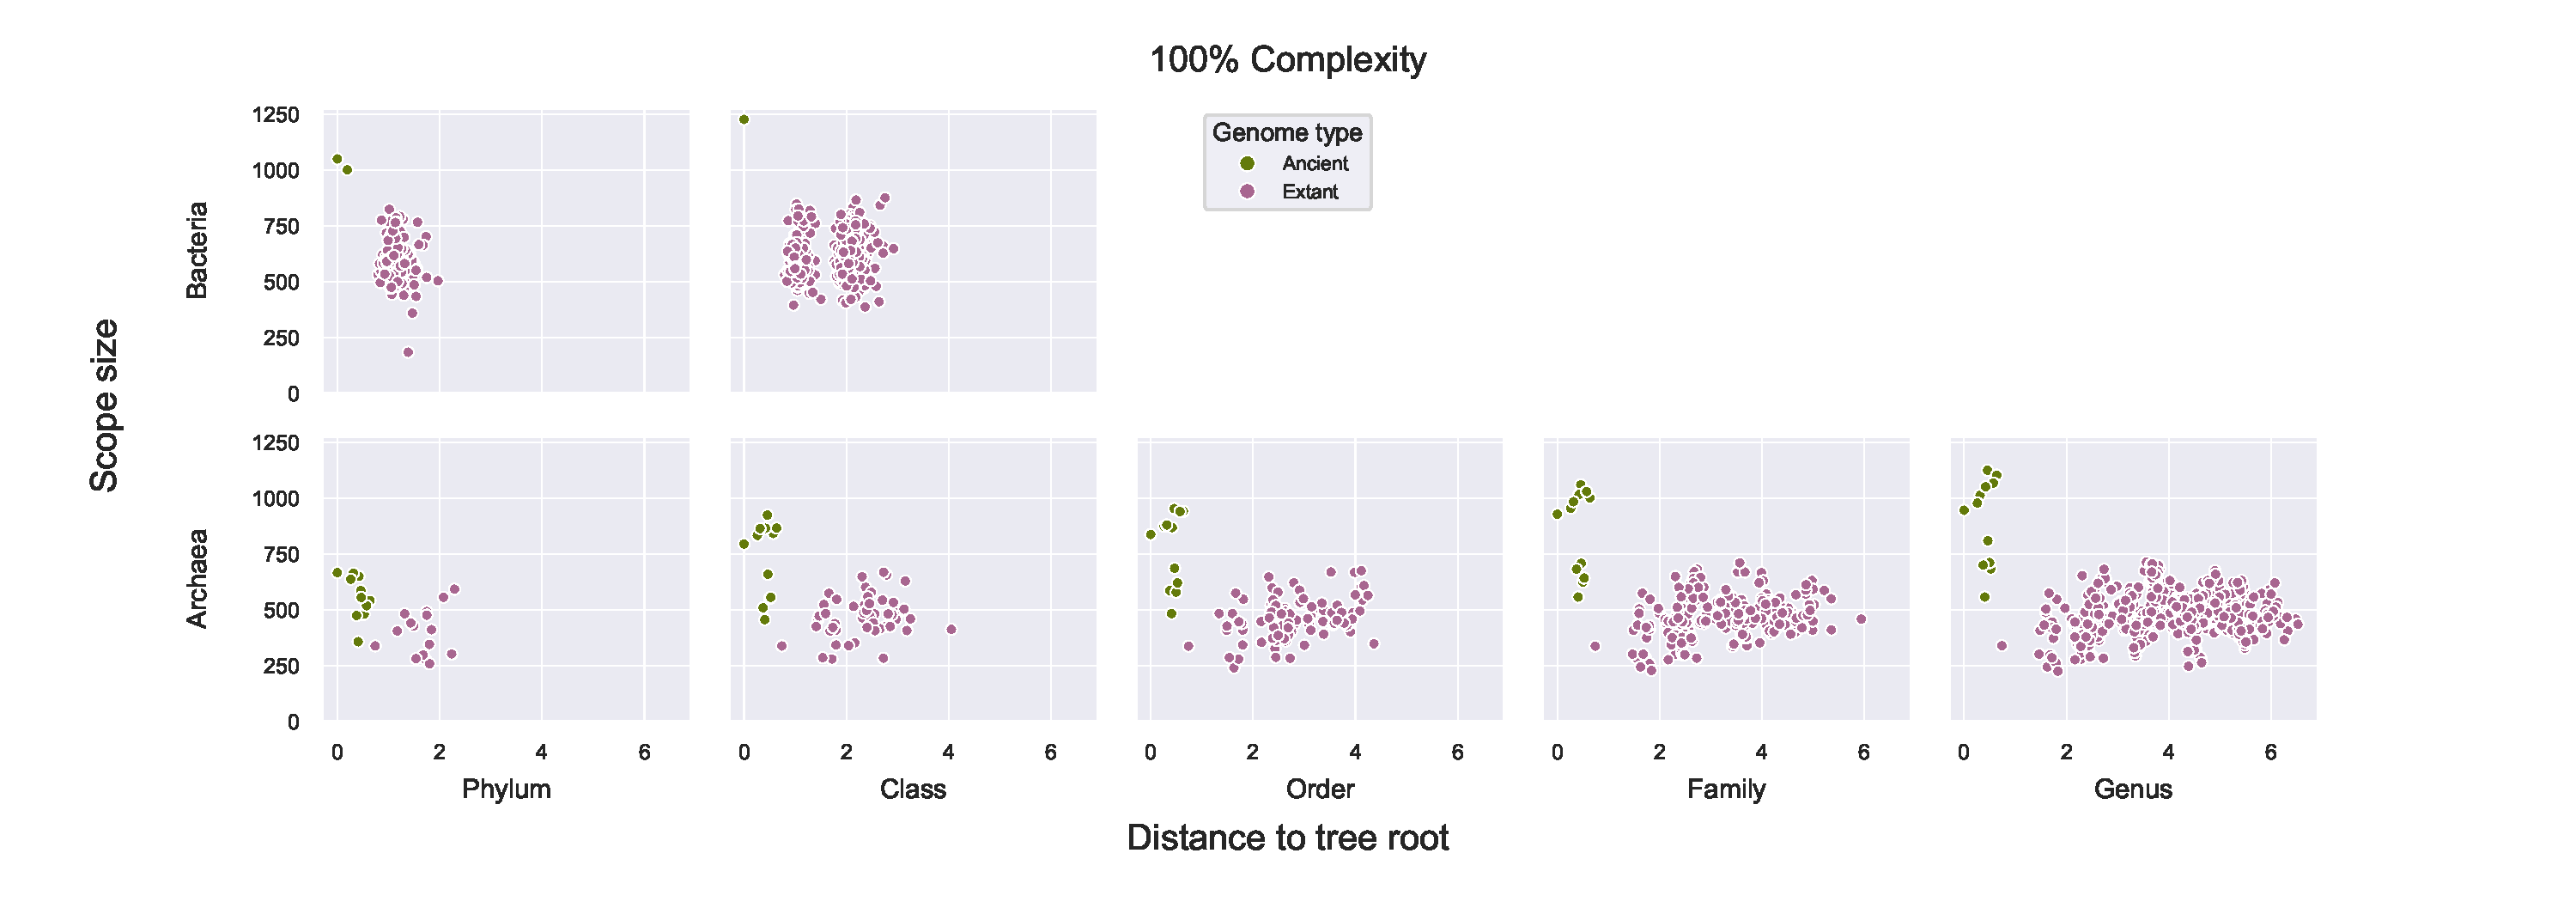
\includegraphics[width=0.95\textwidth]{scopesize_vs_disttoroot/1_ss_rootdist.pdf}
    \caption{100\% complexity}
    \label{1_scopesize}
\end{figure}   

\textbf{For every seed set, per taxonomic level dataset.}

\begin{figure}[H]
    \centering
    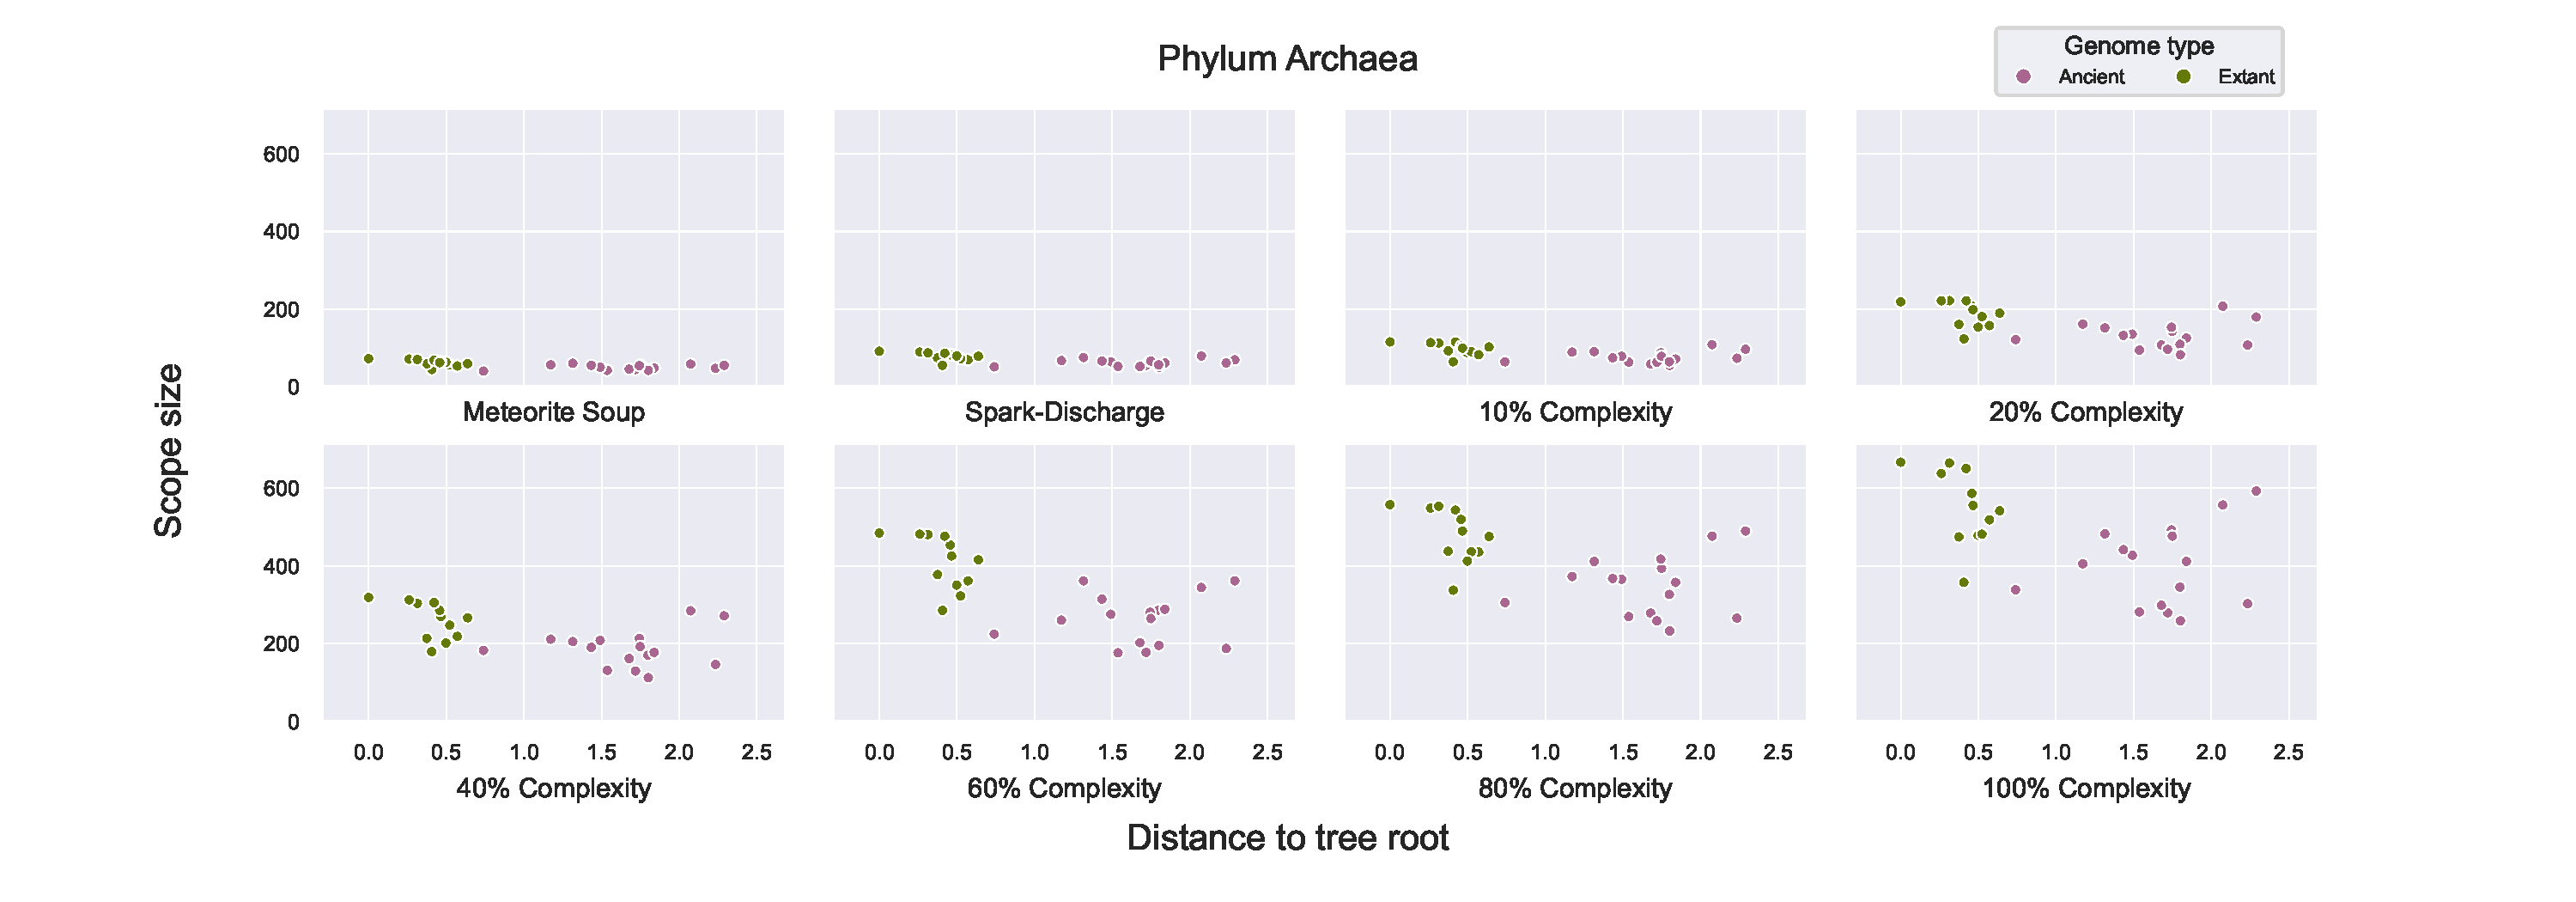
\includegraphics[width=0.95\textwidth]{scopesize_vs_disttoroot/phy4arc_ss_rootdist.pdf}
    \caption{Phylum level archaea}
    \label{phyarc_scopesize}
\end{figure}   

\begin{figure}[H]
    \centering
    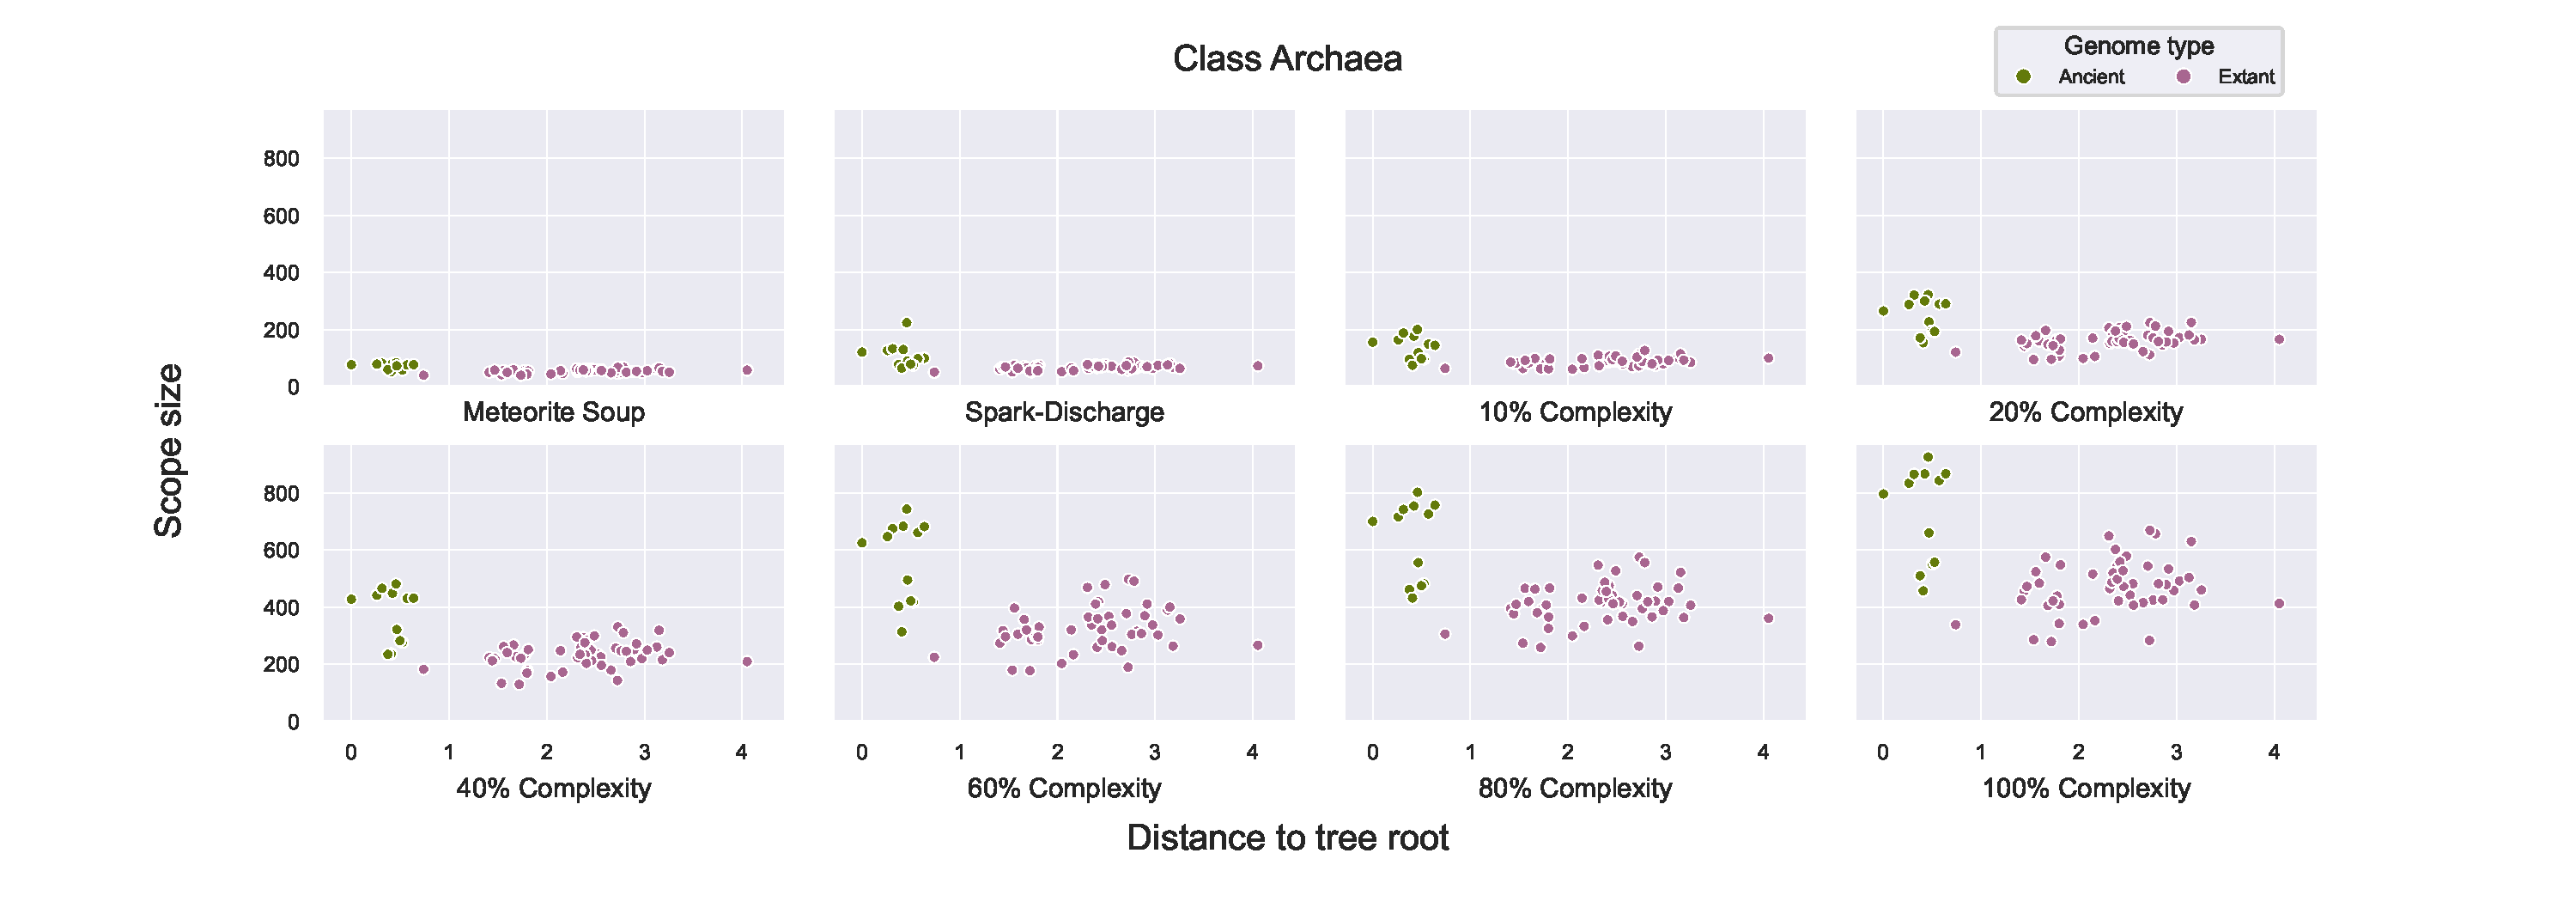
\includegraphics[width=0.95\textwidth]{scopesize_vs_disttoroot/cla4arc_ss_rootdist.pdf}
    \caption{Class level archaea}
    \label{claarc_scopesize}
\end{figure}   

\begin{figure}[H]
    \centering
    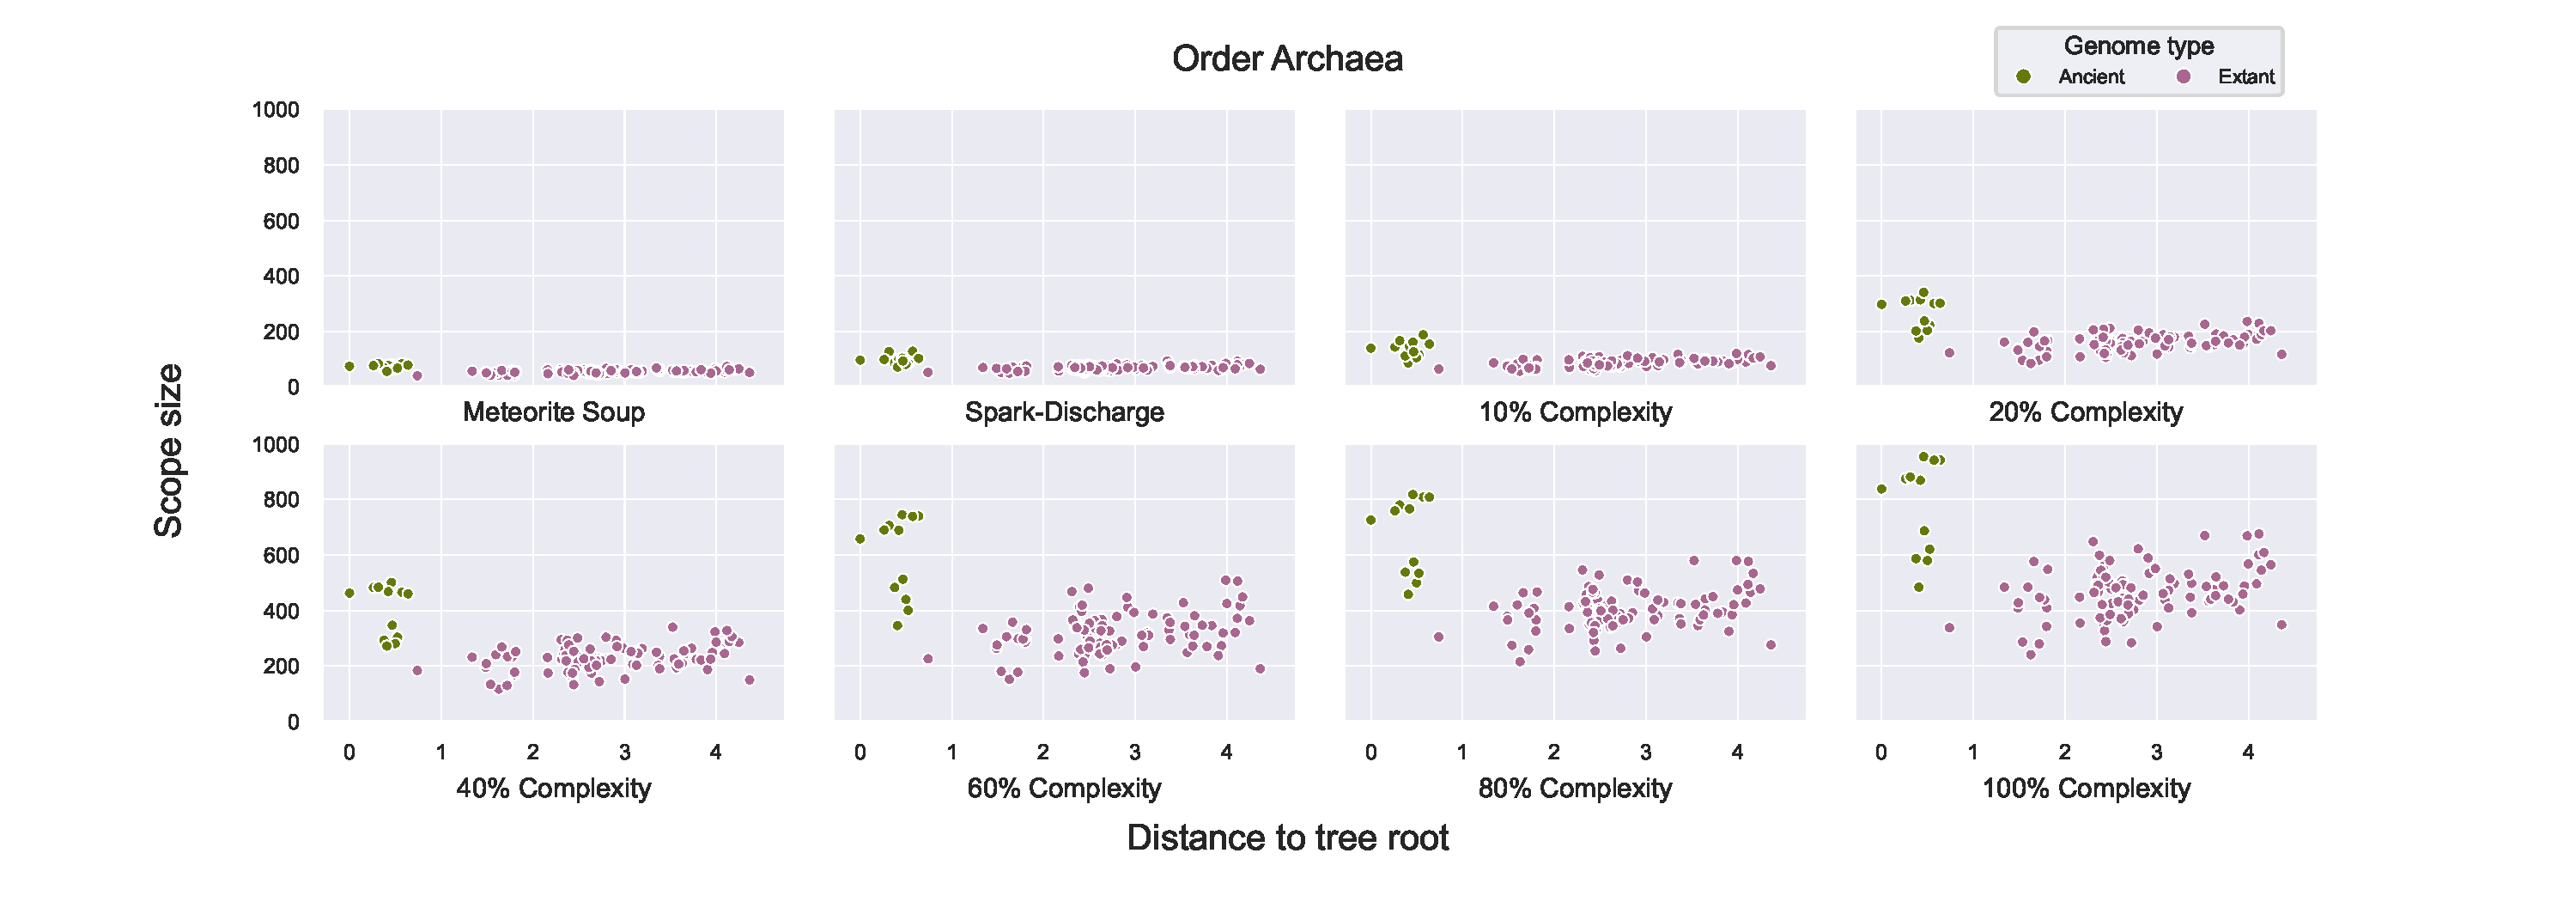
\includegraphics[width=0.95\textwidth]{scopesize_vs_disttoroot/ord4arc_ss_rootdist.pdf}
    \caption{Order level archaea}
    \label{ordarc_scopesize}
\end{figure}   

\begin{figure}[H]
    \centering
    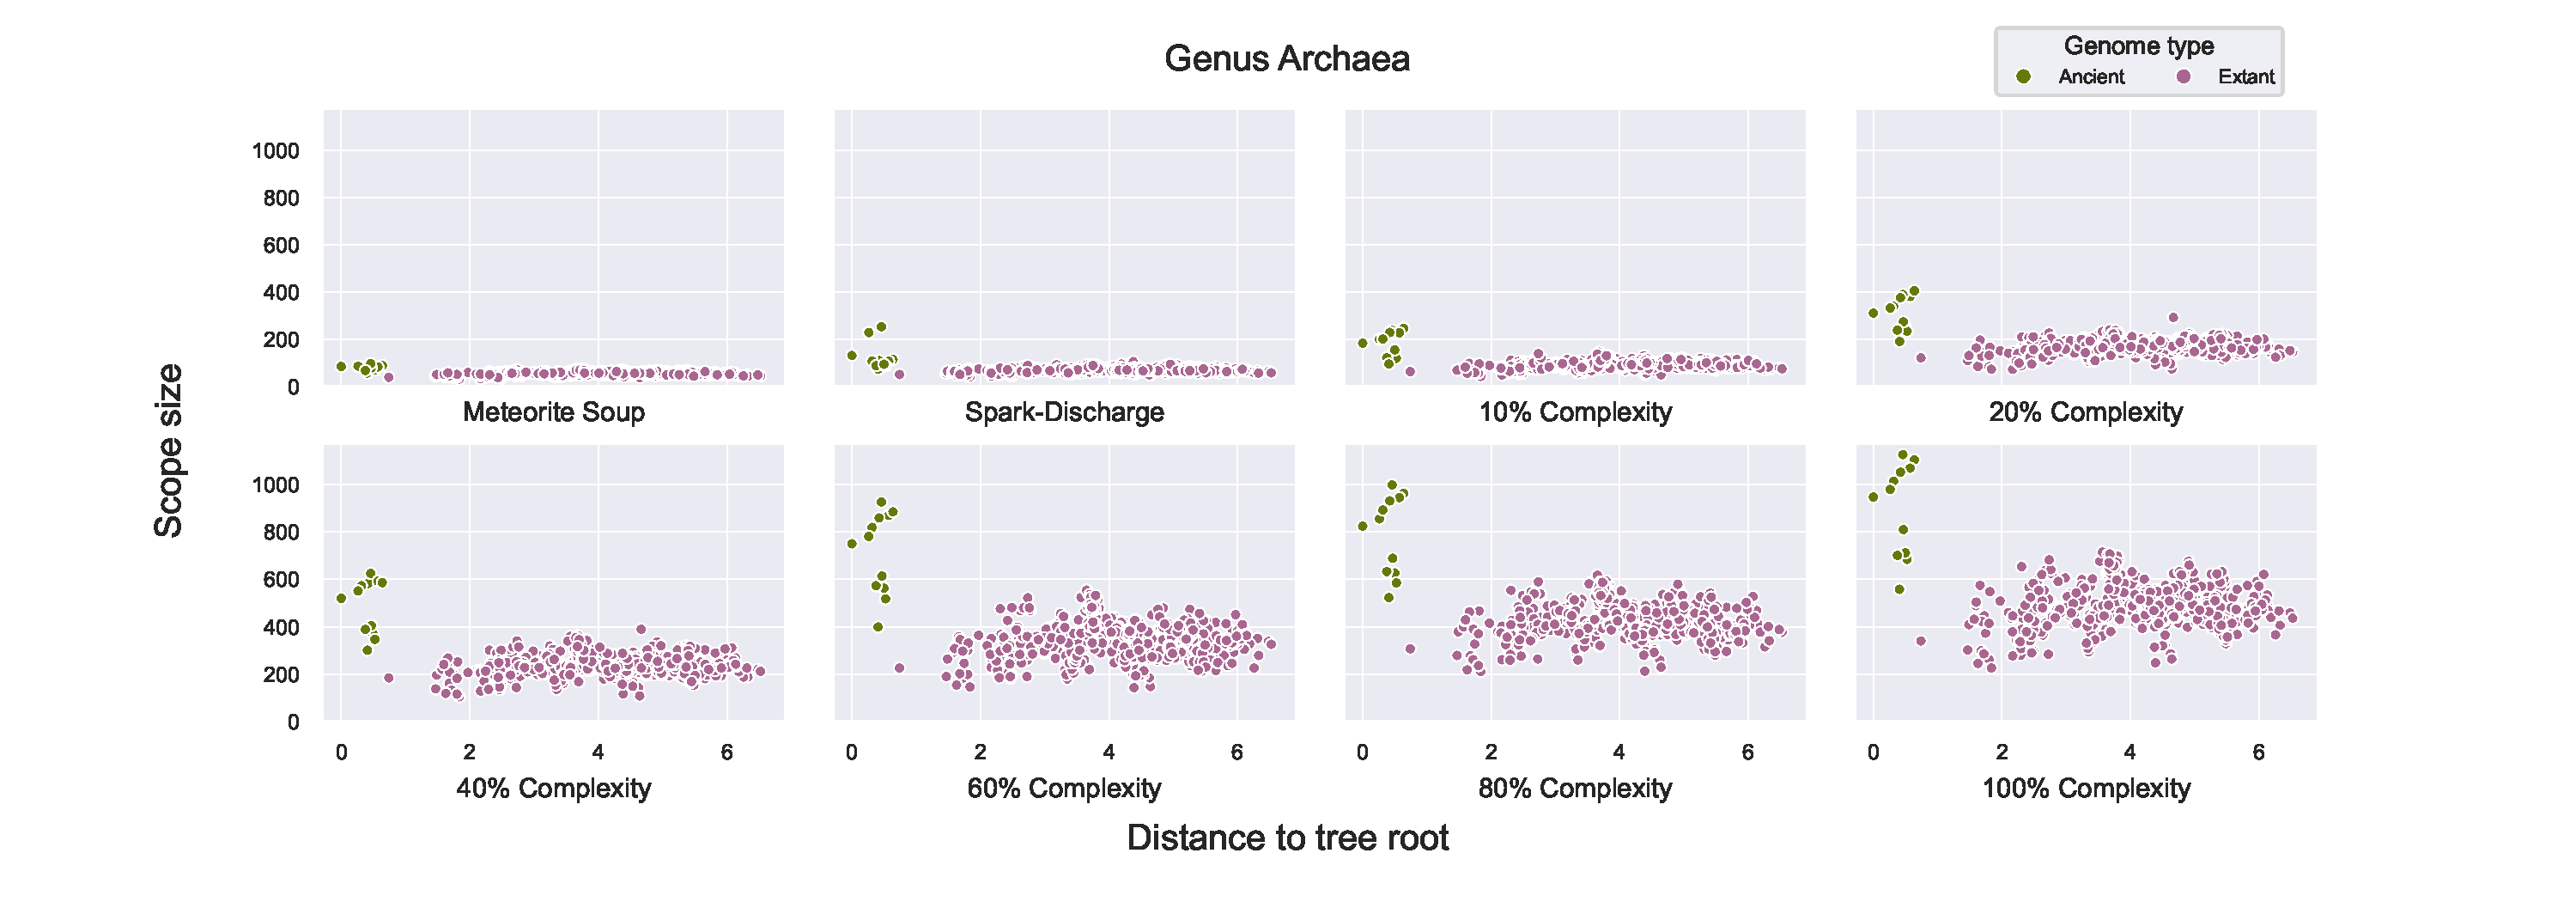
\includegraphics[width=0.95\textwidth]{scopesize_vs_disttoroot/gen4arc_ss_rootdist.pdf}
    \caption{Genus level archaea}
    \label{genarc_scopesize}
\end{figure}   

\begin{figure}[H]
    \centering
    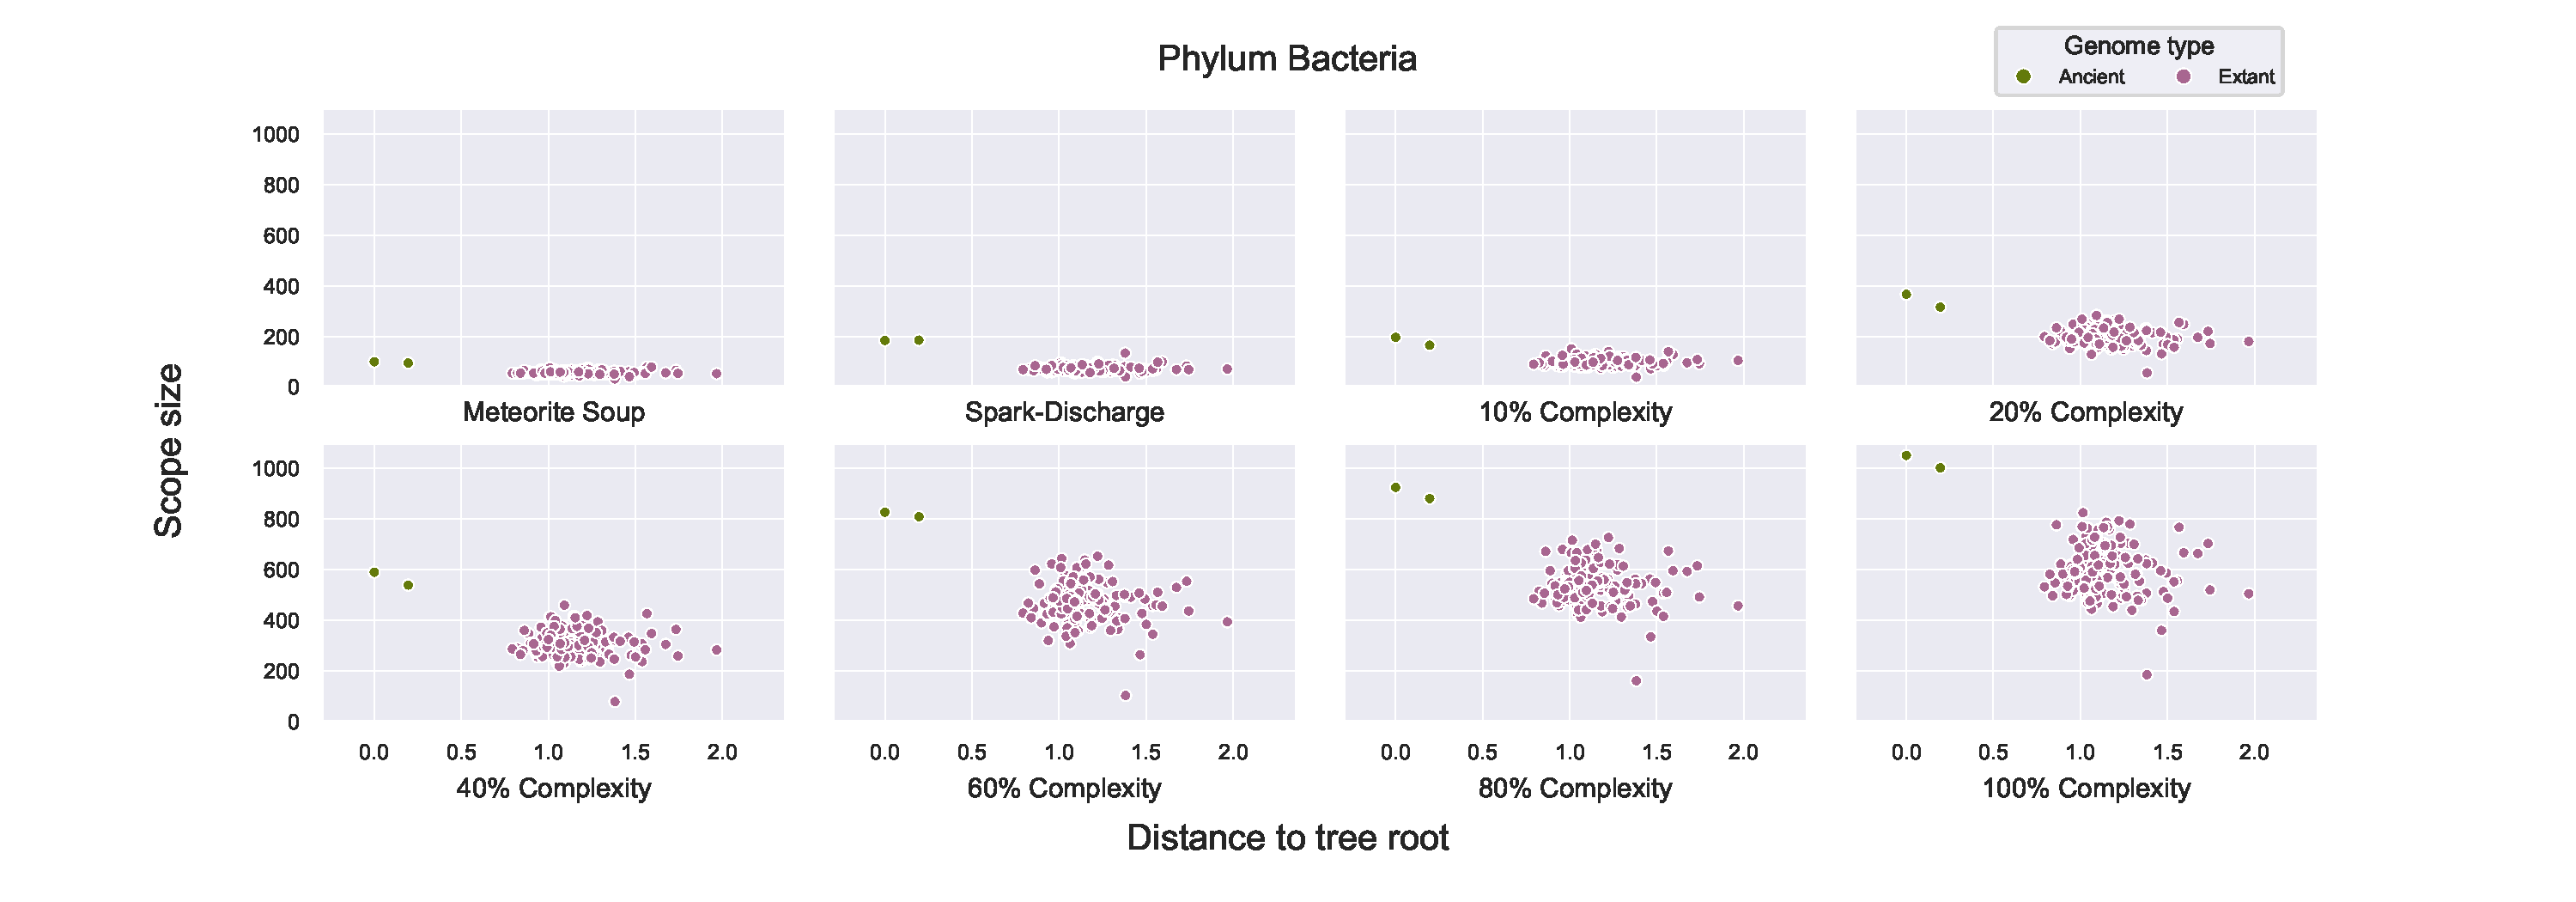
\includegraphics[width=0.95\textwidth]{scopesize_vs_disttoroot/phy4bac_ss_rootdist.pdf}
    \caption{Phylum level bacteria}
    \label{phybac_scopesize}
\end{figure}   

\begin{figure}[H]
    \centering
    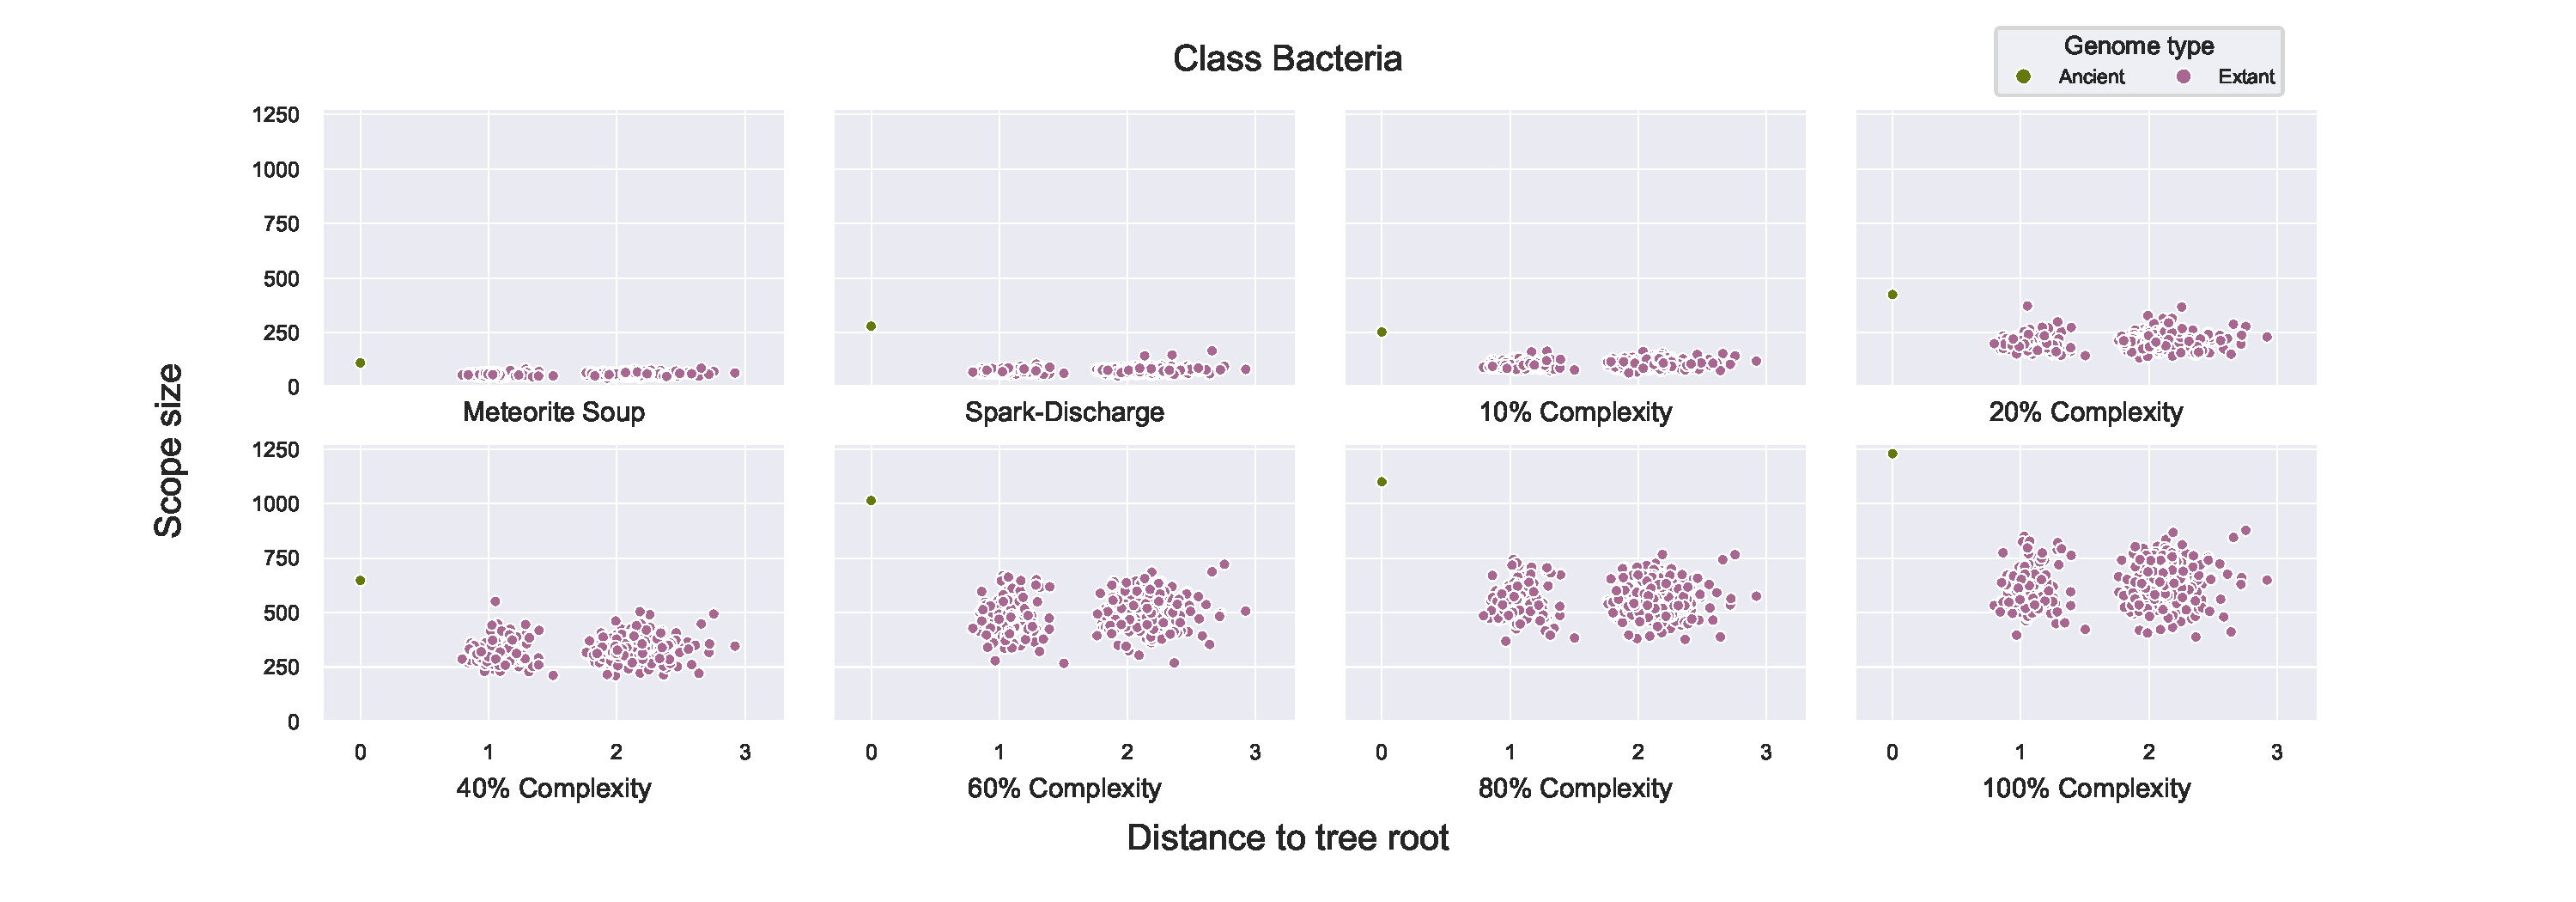
\includegraphics[width=0.95\textwidth]{scopesize_vs_disttoroot/cla4bac_ss_rootdist.pdf}
    \caption{Class level bacteria}
    \label{clabac_scopesize}
\end{figure}   




%\subsection*{A2. Metabolic Network Expansion}
%\addcontentsline{toc}{subsection}{Metabolic Network Expansion}


